% Final report (Architecture Document), D7065E — Embedded Intelligence at the Edge.
% Structure and preamble follow lab-assignment/final_report_template/final_report_template.tex;
% the template's grey guidance notes and bracketed slots are replaced by content, as its
% instructions require. Build: make (latexmk) or make plain (two pdflatex passes).
\PassOptionsToPackage{unicode}{hyperref}
\PassOptionsToPackage{hyphens}{url}
\PassOptionsToPackage{dvipsnames,svgnames,x11names}{xcolor}
%
\documentclass[11pt]{article}
\usepackage{amsmath,amssymb}
\usepackage{lmodern}
\usepackage{iftex}
\ifPDFTeX
  \usepackage[T1]{fontenc}
  \usepackage[utf8]{inputenc}
  \usepackage{textcomp}
\fi
\IfFileExists{microtype.sty}{\usepackage[]{microtype}\UseMicrotypeSet[protrusion]{basicmath}}{}
\makeatletter
\@ifundefined{KOMAClassName}{%
  \IfFileExists{parskip.sty}{\usepackage{parskip}}{%
    \setlength{\parindent}{0pt}\setlength{\parskip}{6pt plus 2pt minus 1pt}}
}{\KOMAoptions{parskip=half}}
\makeatother
\usepackage{xcolor}
\IfFileExists{xurl.sty}{\usepackage{xurl}}{}
\IfFileExists{bookmark.sty}{\usepackage{bookmark}}{\usepackage{hyperref}}
\hypersetup{
  pdftitle={Ventilation Fault Detection, Diagnosis and Graceful Degradation, Architecture Document},
  pdfauthor={Wassim Akachi},
  colorlinks=true,
  linkcolor={RoyalBlue},
  filecolor={Maroon},
  citecolor={Blue},
  urlcolor={Blue}}
\urlstyle{same}
\usepackage[a4paper,margin=2.0cm]{geometry}
\usepackage{longtable,booktabs,array}
\usepackage{calc}
\usepackage{graphicx}
\makeatletter
\def\maxwidth{\ifdim\Gin@nat@width>\linewidth\linewidth\else\Gin@nat@width\fi}
\def\maxheight{\ifdim\Gin@nat@height>\textheight\textheight\else\Gin@nat@height\fi}
\makeatother
\setkeys{Gin}{width=\maxwidth,height=\maxheight,keepaspectratio}
\setlength{\emergencystretch}{3em}
\providecommand{\tightlist}{\setlength{\itemsep}{0pt}\setlength{\parskip}{0pt}}
% Section numbers come from LaTeX, not from the heading text. This file was generated from
% Markdown by pandoc, whose preamble switches numbering off and carries the author's hand-typed
% numbers through as part of each title. That made every number, and every cross-reference to one,
% a literal that nothing checked: "Section 11.6's closed-loop arm" pointed at the register of
% pending measurements for a whole revision, and no build could notice. The format below
% reproduces the hand-typed one exactly -- a period after a section or an appendix letter, none
% after a subsection, one space either way -- so turning numbering on changes no printed character.
\setcounter{secnumdepth}{2}
\usepackage{newunicodechar}
\usepackage{textcomp}
\usepackage{amssymb}
\newunicodechar{°}{\textdegree}
\newunicodechar{₂}{\textsubscript{2}}
\newunicodechar{→}{\ensuremath{\rightarrow}}
\newunicodechar{≤}{\ensuremath{\leq}}
\newunicodechar{≥}{\ensuremath{\geq}}
\newunicodechar{≈}{\ensuremath{\approx}}
\newunicodechar{✓}{\ensuremath{\checkmark}}
\newunicodechar{–}{--}
\newunicodechar{—}{---}
% Added for this document: every non-ASCII character it uses has a declaration, so the build
% does not depend on the input encoding guessing right.
\newunicodechar{σ}{\ensuremath{\sigma}}
\newunicodechar{β}{\ensuremath{\beta}}
\newunicodechar{λ}{\ensuremath{\lambda}}
\newunicodechar{τ}{\ensuremath{\tau}}
\newunicodechar{Σ}{\ensuremath{\Sigma}}
\newunicodechar{Δ}{\ensuremath{\Delta}}
\newunicodechar{×}{\ensuremath{\times}}
\newunicodechar{·}{\ensuremath{\cdot}}
\newunicodechar{²}{\textsuperscript{2}}
\newunicodechar{³}{\textsuperscript{3}}
\newunicodechar{∈}{\ensuremath{\in}}
\newunicodechar{⇒}{\ensuremath{\Rightarrow}}
\newunicodechar{≈}{\ensuremath{\approx}}
\newunicodechar{…}{\ldots}
\newunicodechar{‰}{\textperthousand}
\usepackage{etoolbox}
\AtBeginEnvironment{longtable}{\footnotesize}
\AtBeginEnvironment{tabular}{\footnotesize}
\usepackage{fancyhdr}
\pagestyle{fancy}\fancyhf{}
\rhead{\small D7065E\,--\,Architecture Document}
\lhead{\small Ventilation fault detection}
\cfoot{\thepage}
\renewcommand{\headrulewidth}{0.4pt}
\usepackage{titlesec}
% The label argument is what titlesec prints in front of the title. It printed nothing at all
% while numbering was off, which is why the numbers had to be typed into the titles. A section
% and an appendix letter carry a period after the number and a subsection does not, exactly as
% the typed ones did; the table of contents takes its number from \thesection and so prints it
% without the period, which is LaTeX's own convention and the one place the look changes.
\titleformat{\section}{\Large\bfseries}{\thesection.}{0.6em}{}
\titleformat{\subsection}{\large\bfseries}{\thesubsection}{0.5em}{}
\usepackage{microtype}
\usepackage{pgfplots}
\pgfplotsset{compat=1.16}
% The dynamic view is half again wider than it is tall (1.5:1), which on a portrait page shrinks
% it to the point of being unreadable in print, so it gets a rotated page of its own. The
% component view needed the same treatment at almost 4:1; it is laid out downwards now and is a
% portrait figure at 0.78:1, so it no longer does.
\usepackage{pdflscape}
\usepackage{refcount}
% The span between two labels, inclusive, as a number. Used for the page counts on the title page:
% hand-typed counts are exactly the thing that rots when a paragraph moves.
\newcommand{\pagespan}[2]{\the\numexpr\getpagerefnumber{#2}-\getpagerefnumber{#1}+1\relax}
\setlength{\emergencystretch}{2em}

% --- this document's own helpers -------------------------------------------
% A visible marker for a number that does not exist yet. Nothing in this report may be mistaken
% for a measurement, so every gap is tagged rather than quietly left out.
\definecolor{pendingred}{rgb}{0.70,0.10,0.10}
\newcommand{\pending}[1]{{\color{pendingred}\textbf{[PENDING:} \textit{#1}\textbf{]}}}
\newcommand{\figcap}[1]{\noindent{\footnotesize\emph{#1}}\par\vspace{0.6em}}
% Facts quoted in more than one section, defined once. Changing the test count, the service count
% or the harness's experiment count is one edit in facts.tex, not a grep across sections/.
% Single-sourced facts for this report. Every number defined here is quoted in more than one
% sections/*.tex file, and every one of them has gone stale at least once by being changed in one
% place and not the others. A number that appears once is deliberately not here: it is edited where
% it is written.
%
% Form: a macro holds the number in the form the prose uses -- digits where the report writes
% digits, the English word where the report writes the word. Substituting a macro must never turn
% "Ten compose services" into "10 compose services".
%
% Nothing historical is parameterised. Numbers that record what was measured at a named commit, on
% a named date, or on a patch that was reverted -- the 15/44 probe-order baseline (D.3, I), the 26
% pre-fix false positives (F), the 445 events of the R-5 demo -- keep their literal value even
% where it differs from today's, and must stay literal.
%
% Deliberately not here, and why:
%   * the six rooms. Fixed by Topology.java and by R-7's own design, so it cannot drift; it appears
%     in the heading of 6.1, where a non-expandable macro would reach the table of contents and the
%     PDF bookmarks; and most of its occurrences are derived prose -- "five of six rooms", "the
%     other five rooms", "eight of its ten rooms" -- that one count macro cannot carry.
%   * the five published ports. One occurrence (9, first paragraph), and that sentence enumerates
%     all five ports beside the count, so a macro would let the count drift from its own list.
%   * the per-module test counts in K.2, the harness's 350 s, and its nine result tables. One
%     occurrence each, or ordinal forms ("the ninth is T-28") a count macro cannot carry.
%   * 0 failures and 0 errors. They cannot drift without the build going red.

% --- The unit suite ----------------------------------------------------------
% Tests over the whole Maven reactor. Re-measure:
%   cd project && mvn -o clean test \
%     | grep -E '^\[(INFO|WARNING)\] Tests run:' | grep -v ' -- in ' \
%     | awk -F'[:,]' '{s+=$2} END {print s}'
% The [WARNING] alternative is not optional: Surefire prints a module's summary line as [WARNING]
% rather than [INFO] when that module skipped anything, so matching [INFO] alone silently drops the
% whole of shared/ -- which is nearly half the suite. The ' -- in ' filter drops the per-class
% lines, which would otherwise be counted a second time.
% Changing this number means changing the per-module breakdown in K.2 with it: the two must sum.
\newcommand{\factSuiteTests}{621}

% The day the run above was taken. Two subsections quote that one run; before this file they quoted
% it as two different days.
\newcommand{\factSuiteRunDate}{2026-10-11}

% Reactor modules that have tests -- one fewer than the ten projects the reactor builds, because
% the root POM carries none of its own. Re-measure:
%   cd project && mvn -o clean test \
%     | grep -E '^\[(INFO|WARNING)\] Tests run:' | grep -vc ' -- in '
\newcommand{\factReactorModules}{nine}

% Tests guarded by Assumptions.assumeTrue: the ones that skip when the broker or the database they
% assert against is unreachable, and run when it is up. The suite's skip count is therefore not a
% property of the suite -- it is this number on a bare machine and zero with the stack up -- which
% is why the report quotes this and never a skip count. Re-measure:
%   cd project && grep -rl --include='*.java' Assumptions.assumeTrue . \
%     | xargs grep -h -c '@Test' | awk '{s+=$1} END {print s}'
\newcommand{\factGuardedTests}{eleven}

% ... and how those are spread over the three suites that hold them. Re-measure each with
%   grep -c '@Test' project/shared/src/test/java/se/ltu/d7065e/shared/boundary/<name>.java
\newcommand{\factJournalTests}{eight}   % TimescaleJournalIntegrationTest -- needs PostgreSQL
\newcommand{\factPipelineTests}{two}    % MqttPipelineIntegrationTest -- broker and fault-monitor
\newcommand{\factReconnectTests}{one}   % MqttReconnectIntegrationTest -- needs the broker

% --- Deployment --------------------------------------------------------------
% Services in docker-compose.yml. Re-measure:
%   cd project && grep -cE '^  [a-z0-9-]+:' docker-compose.yml
% Two forms, because the prose needs both at the start of a sentence and inside one. The lowercase
% one is derived from the capitalised one by \lowercase, so there is still only one value to edit
% and the two can never disagree.
\newcommand{\factComposeServicesCap}{Ten}
\newcommand{\factComposeServices}{\expandafter\lowercase\expandafter{\factComposeServicesCap}}

% ... of which this many are built from a folder under project/, rather than being buildsim from
% the sibling buildingsim/ folder or a third-party image. Re-measure:
%   cd project && grep -c 'build: \./' docker-compose.yml
\newcommand{\factAuthoredServices}{seven}

% --- The offline evaluation harness ------------------------------------------
% Experiments evaluation/Main can run, counted as the ids it dispatches. Re-measure:
%   cd project && grep -c '::run;' evaluation/src/main/java/se/ltu/d7065e/evaluation/Main.java
\newcommand{\factExperiments}{ten}

% ---------------------------------------------------------------------------

\begin{document}

\begin{center}
{\LARGE Ventilation Fault Detection, Diagnosis and Graceful Degradation\par}
\vspace{0.5em}
{\large D7065E, Architecture Document\par}
\vspace{1em}
{Project Group 5 (solo): Wassim Akachi\par}
\vspace{0.3em}
{\small v1.1, submission, 2026-10-11\par}
\vspace{0.6em}
{\small\textbf{Report: \pagespan{sec:1}{sec:13end} pages} (Sections \ref{sec:1}--\ref{sec:13},
pp.~\pageref{sec:1}--\pageref{sec:13end}).
Appendices \ref{sec:A}--\ref{sec:K}: \pagespan{sec:A}{sec:Kend} pages, reference only.\par}
\end{center}

\vspace{0.8em}

\begin{center}
\fbox{\parbox{0.93\linewidth}{\footnotesize
\textbf{On the state of the evidence.} The architecture, the physics, the detector, the
supervisor and the dashboard are built and running, and the unit suite is green at
\textbf{\factSuiteTests{} tests, 0 failures, 0 errors}, with \factGuardedTests{} integration tests
skipped by design when nothing is up for them to assert against (Section \ref{sec:10.2}). The \emph{offline
evaluation harness}
(\texttt{project/evaluation/}) is written and has run, so R-1 to R-7 all carry the experimental
evidence their acceptance criteria name (Section \ref{sec:11.2}). \textbf{R-3 is not met; R-1, R-2 and R-7 are
met on the arm their criteria name and fail on the harder arm beside it; R-4, R-5 and R-6 are met.}
R-4 carries both the in-JVM kill experiment and the container-level chaos run, and R-5's case rebuild
has been demonstrated against a live stack \emph{and} is now covered by integration tests that
execute its real SQL. T-15's confusion matrix has been measured, and it is the least flattering
result here: \textbf{one of the four injectable mechanisms is classified correctly}. The
blocked-filter signature is unreachable under this plant's physics, and the sensor-drift branch is
unreachable from \emph{either} sensor mechanism, which is a property of the classifier rather than of
the fault model and was established by adding the mechanism that was supposed to fix it
(Section \ref{sec:7.3}). T-29's optional learned contender has been measured and \textbf{dropped}: at the
monitor's detection rate it costs about twenty times the false alarms and seven times the delay, and
its misses are exactly the monitor's. T-35's reordering of the diagnosis has been measured and
\textbf{not adopted}, for a reason worth more than the change: the third diagnostic signal is blind
after a confirmation rather than merely late (Section \ref{sec:13.6}).
\textbf{No measurement in this report is now outstanding}, which is not the same as every
requirement passing, and Section \ref{sec:11.6} keeps the bound on what each result actually is. Every remaining
gap is marked \pending{what is missing} in place, and Section \ref{sec:11.6} lists all of them in one table. No number in the prose or tables is an estimate: each
comes from a file in the repository, a command I ran, or parameters that are. Figures can lag
their sources, and have.}}
\end{center}

\vspace{1em}

\begin{center}
\fbox{\parbox{0.93\linewidth}{\footnotesize
\textbf{How to read this report, and in what order.} The body is Sections \ref{sec:1}--\ref{sec:13}. Everything whose
job is to be \emph{available} rather than read is in a lettered appendix, cross-referenced from the
exact place in the body where a reader would otherwise go looking. \textbf{No appendix is
load-bearing}: every verdict, every decision and every limitation is stated in the body, and the
appendices carry only the working behind them.

\textbf{The nineteen-page path.} The whole argument is in five places (nineteen pages of the
forty-two), and a reader short of time can stop after them:
\begin{itemize}\tightlist
\item \textbf{\S\ref{sec:1}}, pp.~\pageref{sec:1}--\pageref{sec:1end}: the use case in one sentence, the two nested loops, and
  \emph{where the seven requirements landed} before any detail.
\item \textbf{\S\ref{sec:3}}, pp.~\pageref{sec:3}--\pageref{sec:3end}: the requirements table: each requirement's type, priority,
  measurable acceptance criterion, verdict, and \textbf{the regime that verdict holds in}. Four of
  the seven carry a failing clause and it is in the table, not buried.
\item \textbf{\S\ref{sec:4.5}--\ref{sec:4.6}}, pp.~\pageref{sec:4.5}--\pageref{sec:4end}: every significant decision against the alternative it
  beat and the price paid, then how the architecture grows: the two scaling ceilings, the shard
  boundary, and the one boundary that is \emph{not} a seam.
\item \textbf{\S\ref{sec:11.2} and \S\ref{sec:11.7}}, pp.~\pageref{sec:11.2} and \pageref{sec:11.7}: the measured R-1 to R-7 results, and what
  the compensation costs in energy to buy what it buys.
\item \textbf{\S\ref{sec:13}}, pp.~\pageref{sec:13}--\pageref{sec:13end}: the honest critique: what fails, the mechanism behind each
  failure, and what I would do differently.
\end{itemize}

\textbf{Where the rest lives.}
\begin{itemize}\tightlist
\item \textbf{Appendix \ref{sec:A}} reprints \S\ref{sec:3}'s seven rows with their full evidence column.
  \textbf{Appendix \ref{sec:F}} carries the working behind every verdict in \S\ref{sec:11.2}, and \textbf{Appendix \ref{sec:G}}
  the register of every measurement with the bound on what it actually is.
\item \textbf{Appendix \ref{sec:I}} carries the mechanism behind each finding in \S\ref{sec:13}, and \textbf{Appendix
  \ref{sec:J}} the risk register.
\item \textbf{The remaining appendices} hold supporting depth: \textbf{B} the component,
  code-level and sequence views, \textbf{C} the six rooms, the invented parameters and the REST
  contract, \textbf{D} the diagnosis and its confusion matrix, \textbf{E} the compensation algebra
  and its second lever, \textbf{H} the dashboard evidence frames, \textbf{K} the test plan, the
  suite and the harness.
\end{itemize}
\textbf{One rule for reading the verdicts.} None of them is global. Where a requirement is met on one
occupancy regime and fails on another, both arms are stated wherever the verdict appears, and quoting
either alone misrepresents the result.}}
\end{center}

\vspace{1em}


{
\hypersetup{linkcolor=black}
\setcounter{tocdepth}{3}
% A two-level number is set in a fixed-width box in the contents, and article's default 2.3em is
% narrower than 13.10 and 13.11, which ran into their own titles the moment the numbers became
% real. The box is widened to fit the widest number this document has.
\makeatletter
\renewcommand*\l@subsection{\@dottedtocline{2}{1.5em}{3.2em}}
\makeatother
\tableofcontents
}

\section{Summary}\label{sec:1}

This system runs demand-controlled ventilation over six rooms of an office floor and, on top of
it, a second loop that decides whether that ventilation is still \emph{working}. The guiding
principle is one sentence and it is the thread through every decision that follows: \textbf{a
stuck damper and a full room look identical to a CO₂ controller, and what tells them apart is a
model of what the last command should have achieved.} A controller that sees only concentration
cannot distinguish a room that will not ventilate from a room with more people in it; both read
high. Predicting the response each command owes, and watching the gap between that prediction and
the measurement, turns the fault from an invisible condition into an observable one, which makes
the autonomous part an inference problem rather than a threshold, and makes fault injection and
degraded operation the use case itself rather than an experiment bolted on at the end.

The system is therefore \textbf{two nested loops}, and the outer one is the contribution.

\begin{longtable}[]{@{}
  >{\raggedright\arraybackslash}p{(\columnwidth - 4\tabcolsep) * \real{0.26}}
  >{\raggedright\arraybackslash}p{(\columnwidth - 4\tabcolsep) * \real{0.10}}
  >{\raggedright\arraybackslash}p{(\columnwidth - 4\tabcolsep) * \real{0.64}}@{}}
\toprule
\textbf{Loop} & \textbf{Period} & \textbf{Closes because} \\
\midrule
\endhead
Inner, control (\texttt{dcv-controller}) & ≈ 1 s & A damper command changes airflow, which
changes CO₂, which the controller reads next \\
Outer, supervision (\texttt{fault-monitor} + \texttt{supervisor}) & ≈ 60 s & A confirmed fault
changes the control strategy, which changes the commands, which changes the residual the monitor
reads next \\
\bottomrule
\end{longtable}

The inner loop is deliberately a plain rule: CO₂ in, damper position out, with hysteresis and a
freshness check. That is not an omission but the point. Demand-controlled ventilation is a solved
problem, and making the inner rule cleverer would have bought nothing the course grades; the
interesting and unsolved question is what happens when the actuator the clever rule depends on
has quietly stopped working. Keeping the inner loop simple also keeps it \emph{verifiable}, which
matters because the outer loop judges it: an observer that has to model a sophisticated
controller inherits that controller's complexity as model error.

\begin{longtable}[]{@{}
  >{\raggedright\arraybackslash}p{(\columnwidth - 2\tabcolsep) * \real{0.26}}
  >{\raggedright\arraybackslash}p{(\columnwidth - 2\tabcolsep) * \real{0.74}}@{}}
\toprule
\textbf{Field} & \textbf{Value} \\
\midrule
\endhead
\textbf{Project title} & Ventilation Fault Detection, Diagnosis and Graceful Degradation \\
\textbf{Team members} & Wassim Akachi (project group 5, solo) \\
\textbf{Use case} & Demand-controlled ventilation that detects, diagnoses and survives faults in
its own equipment \\
\textbf{Repository} & \url{https://github.com/eduni-pro/202608-d7065e}, subfolder \texttt{project/} \\
\textbf{Version / date} & v1.1, submission, 2026-10-11 \\
\bottomrule
\end{longtable}

This is a solo project, so no contribution statement is included: the course requires one only
where a pair submits a single system, and every decision, measurement and line of code recorded
here is my own.

\textbf{Where it landed, before the detail.} Two of the seven requirements are met outright. Three
more pass on the arm their acceptance criterion names and fail on the harder arm beside it, and
they are reported as \emph{two} numbers rather than one, because a single verdict would have to
pick which regime to be silent about. \textbf{R-3 is the one that fails everywhere (0.55
confirmed false alarms per fault-free simulated week against a budget of one, and a worst week of
6, which is the criterion it is scored on) and R-1's, R-2's and R-7's harder arms all have that
same false-alarm rate somewhere in their causes.} One defect,
surfacing four times, is a more useful thing to know about this system than four defects would be,
and §\ref{sec:11} reports it that way rather than softening it. The regime that separates the arms is not
the same in each case and is named with each result: for R-2 and R-7 it is \emph{occupancy} (the
drawn weekday passes, design occupancy does not), while for R-1 it is the \emph{protocol}, which
detects 20 of 20 at a p95 of 6 min when the damper is stepped deliberately and 15 of 20 at 257 min
when the fault must be found in the closed loop that is also compensating for it.

\subsection{Changes since the proposal}\label{sec:1.1}

Three things changed, and each was forced by a decision I had to make rather than by a change of
mind. The accepted proposal (2026-09-18) carried one examiner condition, \emph{``make sure to
include several rooms''}, and answering it honestly is what drove all three.

\textbf{1. The coupling topology: six independent rooms became one shared air handler with a
damper per room.} ``Several rooms'' can be satisfied by replication, six copies of the single-room
spike with nothing one room can do to another, and the implementation plan's risk register names
exactly that as the failure to avoid. ADR-0008 therefore weighed three couplings and chose
\textbf{option B}: one air-handling unit \texttt{AHU-A120}, one damper per room, and a
proportional flow split, sized 43 \% above the sum of the six rooms' design flows, but only
0.4 \% above it at the normal fan speed of 0.7, so that \emph{the only way one room gets more air
is if another damper closes} and the headroom is a compensation budget rather than normal slack. Rejected: option A
(independent rooms, a fan each), which makes R-7 hold by construction and its experiment measure
nothing; and option C (option B plus inter-room air exchange), which is the proposal's literal
wording but whose exchange coefficient, the one parameter nothing can measure, would be what
decides whether R-2 passes.

\textbf{2. ``Over-ventilate the neighbour'' became ``over-drive the shared handler and trim the
neighbours' dampers''.} The proposal said the supervisor would compensate by over-ventilating the
faulted room's neighbour, which presumes air moves between rooms. Under option B it does not:
rooms are coupled through the \emph{duct}, not through the wall. The mechanism that replaces it is
better, not merely different, and Section \ref{sec:7.4} derives it: one common trim on the healthy dampers
plus one raise of the shared fan speed holds every healthy room's airflow exactly where it was
while multiplying the faulted room's flow by the reciprocal of the trim. The cost is a stated
bound (a damper stuck fully shut has no air path and cannot be reached at all), and that bound is
reported with R-2 rather than hidden.

\textbf{3. Fan power moved from a per-room signal to a plant signal, and that is what makes
discrimination possible at all.} In the proposal's sketch each room had its own fan, so fan power
was a local quantity and a blocked filter was a local anomaly. With one shared unit, fan power
belongs to the plant. That single relocation is what gives the monitor a \emph{cross-room} signal:
a blocked filter starves all six rooms at once and raises power per unit of flow, while a stuck
damper moves one room's residual and leaves plant power flat. Without it, separating those two
faults would have needed a fourth invented signal, which the risk register explicitly forbade.

One thing did \emph{not} change and deserves saying so: the detection method. The proposal
proposed a predicted step response, a residual and a CUSUM (one-sided then, two-sided now that
§\ref{sec:7.3}'s guarded lower arm has been added), and the week-37 spike
(Section \ref{sec:11.1}) found the separation so large that the design question moved from ``can this be
detected'' to ``how few false alarms can it be detected with''.\label{sec:1end}

\section{Use case and building context (BuildSim)}\label{sec:2}

\textbf{The building.} The system controls six rooms on level 0 of the A-building, modelled in
\textbf{BuildSim}. BuildSim is the \emph{shared state} of the cyber-physical system: it owns the
building model (levels, rooms, equipment), exposes a REST API to register devices and to read and
write their state, and streams live state to a 3D web viewer. BuildSim is not modified; it is
instrumented. That seam is the boundary between the physical half of a cyber-physical system (the
building, behind BuildSim's API) and the cyber half (my processes), and keeping it clean is what
would let the same software later drive a real air handler.

\textbf{BuildSim provides the rooms and no physics}, so the air, the people and the plant are all
simulated here (Section \ref{sec:6}). How the processes use BuildSim is fixed and narrow:

\begin{itemize}
\tightlist
\item \texttt{physics-simulator} is the \emph{only} process that touches the environment. It reads
  the current damper and fan-speed actuator state from BuildSim, advances the CO₂ balance and the
  air handler, and writes the resulting sensor values back. This is what closes the loop.
\item \texttt{co2-sensor} reads the six room CO₂ values and the one air handler's fan power from
  BuildSim and publishes them to the broker. It emulates devices that observe and report; it does
  not generate values.
\item \texttt{damper-actuator} applies validated commands to BuildSim: the six dampers and the
  one fan speed. BuildSim remains the single source of truth for actuator state.
\item \texttt{dashboard} repaints BuildSim's own floorplan as room layers, and \texttt{supervisor}
  writes work orders as BuildSim alerts. Those two are the only writers of operator-facing state.
\end{itemize}

\textbf{Actors.} The \textbf{facilities technician} receives the work order and repairs the
damper, which is the only external event that can clear a latched diagnosis. \textbf{Room
occupants} are the CO₂ source and the people whose comfort R-2 protects; they influence the system
only by being present. Neither actor is on the control path: both loops run autonomously.

\textbf{The scenario the demo tells.} At 09:00 the meeting room A115 is booked and ten people
arrive. CO₂ climbs past 800 ppm, the controller opens the damper, and at 1020 ppm it commands the
damper fully open. The damper is frozen at 0.15, so the airflow never changes and CO₂ keeps
rising. The monitor saw the same command, predicted the fall that opening from 0.15 to 1.00 owed,
and instead watches the gap grow until the accumulated residual is too large and too persistent to
be sensor noise. Plant fan power flat argues against a blocked filter; a correct overnight decay
to outdoor level argues against a drifting sensor; the monitor publishes a confirmed
\texttt{STUCK\_DAMPER}. The supervisor degrades A115 so the inner loop stops commanding it, trims
the five healthy dampers and raises the shared fan so the five keep the airflow they had, and
raises a work order on the 3D view. A115's CO₂ falls back under the limit, and \textbf{the
diagnosis stays latched}, because the thing that made the residual shrink was the response to the
diagnosis, not a repair. That last sentence is the hardest property in the design and the one the
oral will probe.

\textbf{Why it matters.} A demand-controlled system that silently stops ventilating is worse than no
demand control at all: the fixed-schedule system it replaced would at least have kept moving air.
Faults in ventilation equipment are undramatic: a damper that no longer modulates produces no
alarm, no noise and no visible symptom, only a room that is slightly worse to be in for however many
weeks pass before somebody complains. A loop that can tell ``this room is busy'' from ``this room is
broken'' is what makes demand control safe to deploy, and that is the whole use case. Ventilation
fault detection is also only one of several systems that would run on this same building model
(fire detection, access control and energy management would each be their own), and this report
designs one of them.

\section{Requirements}\label{sec:3}

The requirements are the root of the traceability thread: each is a \textbf{testable} statement
with a stable ID, written in \textbf{EARS}\footnote{\textbf{E}asy \textbf{A}pproach to \textbf{R}equirements
\textbf{S}yntax, from Rolls-Royce's airworthiness work: A.~Mavin, P.~Wilkinson, A.~Harwood and
M.~Novak, ``Easy Approach to Requirements Syntax (EARS)'', \emph{2009 17th IEEE International
Requirements Engineering Conference}, pp.~317--322,
\href{https://doi.org/10.1109/RE.2009.9}{doi:10.1109/RE.2009.9}; practitioner guide at
\url{https://alistairmavin.com/ears/}. Of its six patterns this report uses four: the three
preconditions below, and the ubiquitous form that takes none.} form (an optional \texttt{When} event, \texttt{While}
state or \texttt{If} unwanted-condition precondition, then \emph{the system shall} a response),
traced to a design element in Sections \ref{sec:4}–\ref{sec:9} and to a verification in Section \ref{sec:10}. The authoritative
repository's copy is \texttt{project/REQUIREMENTS.md}; this section adds each
requirement's verdict and the regime it holds in.

The \textbf{verdict column is the honest one}, and it is the most important column in this report.
The offline evaluation harness has now run, so all seven requirements carry the experimental
evidence their acceptance criteria name, and \textbf{four of the seven carry a failing clause}:
R-1, R-2, R-3 and R-7, which the column says in its first words rather than at the end of a
paragraph. Two of those four fail on the harder of two arms and pass on the one their criterion
names, and both arms are stated. R-4's evidence is now a container kill as well as an in-JVM one,
and R-5's is a live rebuild \emph{and} an integration test that executes its SQL.

\begin{longtable}[]{@{}
  >{\raggedright\arraybackslash}p{(\columnwidth - 10\tabcolsep) * \real{0.05}}
  >{\raggedright\arraybackslash}p{(\columnwidth - 10\tabcolsep) * \real{0.07}}
  >{\raggedright\arraybackslash}p{(\columnwidth - 10\tabcolsep) * \real{0.06}}
  >{\raggedright\arraybackslash}p{(\columnwidth - 10\tabcolsep) * \real{0.28}}
  >{\raggedright\arraybackslash}p{(\columnwidth - 10\tabcolsep) * \real{0.25}}
  >{\raggedright\arraybackslash}p{(\columnwidth - 10\tabcolsep) * \real{0.29}}@{}}
\toprule
\textbf{ID} & \textbf{Type} & \textbf{Pri.} & \textbf{Statement (EARS)} & \textbf{Acceptance
criterion, and how it is verified} & \textbf{Verdict, and the regime it holds in} \\
\midrule
\endhead
R-1 & Func. & Must & \emph{When} a damper stops responding to commands, the system shall confirm the fault. &
p95 confirmation ≤ 15 min after the first ignored command; injection harness, ≥ 20 runs &
\textbf{Met as specified; not met in closed loop} \\*
R-2 & Func. & Must & \emph{While} a fault is latched, the system shall keep the affected zone below 1000 ppm by
compensation. & Zone CO₂ ≤ 1000 ppm for ≥ 95 \% of occupied minutes during the fault; end-to-end
scenario test & \textbf{Met on the case it covers; not met at design occupancy} \\*
R-3 & Non-f. & Must & The monitor shall raise no more than one false alarm per simulated week. & ≤ 1
\texttt{FaultConfirmed} in a 7-day fault-free replay, scored on the \emph{worst} week; replay test
on a fixed seed & \textbf{Not met} \\*
R-4 & Non-f. & Must & \emph{While} readings are stale beyond three intervals, the monitor shall report unavailable
and issue no diagnosis. & State is \texttt{BLIND}, zero fault events published; fault injection,
kill \texttt{co2-sensor} & \textbf{Met, in-JVM and at container level} \\*
R-5 & Non-f. & Must & The system shall make every diagnosis reconstructable. & Inputs, command, residual series,
classification and timestamp recoverable for any \texttt{caseId}; rebuild a case from the journal &
\textbf{Built, demonstrated live against the deployed stack, and now covered by integration
tests} \\*
R-6 & Non-f. & Should & The system shall identify the zone count at which the monitor misses its interval. &
Sustained zone count where the p95 monitor cycle exceeds 60 s is reported; scaling experiment to
breaking point & \textbf{Met, with an extrapolated answer}. And the deployed ceiling is a
different and far smaller number \\*
R-7 & Non-f. & Must & \emph{While} a fault is latched in one room, the system shall keep control and diagnosis of
every other room unchanged. & Zero fault events and no control-mode change in the other five, their
CO₂ \emph{and their airflow} inside the healthy-run band; injection in one room, ≥ 3 rooms rotated
as the injected one & \textbf{Met on the drawn weekday; not met at design occupancy} \\
\bottomrule
\end{longtable}

\textbf{No requirement here is Regulatory, and that is a gap rather than an absence.} Five of the
seven are non-functional, which is the right shape for a system whose interesting claims are about
latency, false-alarm rate, auditability, scale and isolation. But R-2's 1000 ppm is exactly the kind
of number a regulation supplies rather than a designer, and this report asserts it without a source.
Grounding it in the Swedish indoor-air guidance it is plainly borrowed from would convert R-2's
threshold from an invented parameter into a cited one, and §\ref{sec:13.3}, which owns the fact that every
physical parameter here is invented, would have one fewer row.

\textbf{Every measured figure behind those verdicts is in §\ref{sec:11.2}}, one row per requirement, and
\textbf{Appendix \ref{sec:A}} carries the same seven rows with their evidence column in full. The two failing
pairs are the ones to read twice: R-1 and R-7 pass on the arm their own criterion names and fail on
the harder arm beside it, and both arms are stated wherever either appears.

The verdict column above is the short form. \textbf{Appendix \ref{sec:A} reprints the same seven rows with
their full evidence column}, naming the verification each verdict rests on; §\ref{sec:11.2} reports the
experiments themselves.

\subsection{The tension these requirements set up}\label{sec:3.1}

R-2 and R-7 pull against each other, and that is deliberate. R-2 needs a physical lever that
reaches a faulted room from outside it; every such lever risks disturbing the rooms R-7 says must
stay unchanged. With six independent fans there would be no tension and nothing to design: R-7
would hold because nothing couples the rooms, and R-2 would have no mechanism. The shared air
handler creates the tension, and resolving it is the supervisor's whole job (Section \ref{sec:7.4}). R-1 and
R-3 pull against each other in the same way, through a single number: lowering the CUSUM limit
\texttt{h} detects sooner and cries wolf more often. Section \ref{sec:11.1} reports that trade-off as
measured rather than asserted, and §\ref{sec:11.2} now reports a sharper version of the same tension that was
not visible when this was written: the binding knob turned out to be not \texttt{h} but what the
CUSUM's \emph{reference} is, and the setting of it that meets R-3 outright takes R-1's closed-loop
detection from 15 of 20 to 1 of 20 (ADR-0010).

\subsection{Gaps with no requirement ID}\label{sec:3.2}

Kept visible rather than discovered during marking. Each is real work with no ID attached, so
nothing in the table above constrains it and no test can name an ID for it.

\begin{itemize}
\tightlist
\item \textbf{Data quality.} R-4 covers \emph{stale} readings only, and only insofar as staleness
  drives \texttt{BLIND}. Nothing requires duplicate suppression, out-of-order handling, or defines
  what the \texttt{quality} field in \texttt{readings/\{zone\}/co2} must mean.
\item \textbf{The dashboard.} No requirement states what the 3D view must show, how fresh it must
  be, or what counts as the fault being visible. Its verification is ``screenshot evidence for the
  report'', which is a deliverable and not a criterion.
\item \textbf{R-2's bound.} That a damper stuck fully shut must produce a work order rather than an
  attempted compensation is recorded in ADR-0008 and asserted by a unit test, but it is not itself
  a requirement, so no acceptance criterion covers it.
\end{itemize}

\textbf{Traceability.} The five architecture viewpoints map onto this document so that nothing is
left unverified: \emph{context} (4.1), \emph{functional} (4.2–4.5), \emph{information} (5–6),
\emph{behavioural} (8), \emph{deployment} (9). Section \ref{sec:10} closes the loop from each requirement
back to a verification, and Section \ref{sec:11.6} lists every verification that has not yet run.\label{sec:3end}

\section{Architecture}\label{sec:4}

\emph{This section carries three subsections beyond the template's four, so its numbering runs
one ahead from 4.3 onwards. The template's \textbf{4.3 Component diagram} is \S\ref{sec:4.4} here, and its
\textbf{4.4 Design decisions and alternatives} is \S\ref{sec:4.7}. Nothing is omitted: \S\ref{sec:4.3} adds the
authority separation, \S\ref{sec:4.5} the two code-level diagrams, and \S\ref{sec:4.8} how the architecture grows,
all three of which the architecture needs and none of which the template has a slot for.}

\subsection{Context diagram (C4 Level 1)}\label{sec:4.1}

The context view fixes the \textbf{system boundary}. The system reads and commands the building
only through BuildSim; the technician receives a work order and, by repairing the damper, is the
only actor who can clear a latched case; occupants are sensed, not connected. Nothing internal
appears.

\begin{center}\includegraphics[width=0.58\textwidth]{figures/context.pdf}\end{center}
\figcap{C4 System Context (Level 1), from \texttt{project/diagrams/context.d2}. Person and
software-system elements; every arrow is a directed relationship labelled with its purpose and
protocol.}

\subsection{Container diagram (C4 Level 2)}\label{sec:4.2}

Each box is one Docker container, one service in \texttt{docker-compose.yml} and one folder under
\texttt{project/}. That 1:1 mapping is a hard constraint of the implementation plan, not a
coincidence, and it is what keeps the diagram from drifting from the code: adding a box means
adding a folder and a service, which is why the fan-speed command is applied by
\texttt{damper-actuator} rather than by a container of its own (Section \ref{sec:4.7}).

\textbf{\factComposeServicesCap{} compose services, \factAuthoredServices{} of them project-authored}: \texttt{physics-simulator},
\texttt{co2-sensor}, \texttt{damper-actuator}, \texttt{dcv-controller}, \texttt{fault-monitor},
\texttt{supervisor} and \texttt{dashboard}, plus \texttt{buildsim} from the \texttt{buildingsim/}
folder of the same repository and the third-party images \texttt{mosquitto} and
\texttt{timescaledb}, configured under \texttt{project/deploy/}. Two folders are deliberately
\emph{not} containers (\texttt{shared/} is a library and \texttt{evaluation/} the offline harness),
which is the entire reason the folder set is larger than the service set, and the mapping stays
1:1 for all \factAuthoredServices{}.

\begin{center}\includegraphics[width=\textwidth,height=0.70\textheight,keepaspectratio]{figures/container.pdf}\end{center}
\figcap{C4 Container diagram (Level 2), from \texttt{project/diagrams/container.d2}. The dashed
boundary is the system in scope; BuildSim is external; every arrow carries its protocol. The
figure is service-for-service identical to \texttt{project/docker-compose.yml}.}

The loop the figure describes is the one that makes this a cyber-physical system rather than a
dashboard. \texttt{physics-simulator} reads actuator state from BuildSim, advances the physics and
writes sensor values back; \texttt{co2-sensor} reads those values and publishes them;
\texttt{dcv-controller} commands a damper position; \texttt{damper-actuator} applies it to
BuildSim; and that actuator change alters the environment the simulator advances on its next tick.
The outer loop rides the same bus one order of magnitude slower.

The technician writes into the system in two places. One reports the equipment
serviced to \texttt{dashboard}, which is the only exit from a latched case; the other is a small
HTTP fault control surface on \texttt{physics-simulator} (\texttt{POST}, \texttt{GET} and
\texttt{DELETE} on \texttt{/faults}) that injects, lists and clears a fault in the running
plant. The second is what makes a recovery demonstrable rather than merely described: the
scenario can be changed and the damper repaired without restarting the stack. Both ports are
published on \texttt{127.0.0.1} only.

\subsection{Authority separation: who may act}\label{sec:4.3}

\textbf{\texttt{fault-monitor} raises events and never commands. \texttt{supervisor} is the only
component that acts.} This is the single most important structural decision in the system and it
is worth being explicit about why, because the two halves could obviously have been one process.

\begin{itemize}
\tightlist
\item \textbf{A crashing monitor must not be able to stop ventilation.} Diagnosis is the
  speculative, model-dependent, newest and least-trusted code in the system. Control is the part
  that keeps people breathing. If they share a process, a null pointer in the classifier takes the
  damper commands down with it. Split, the worst a dead monitor can do is stop producing
  diagnoses, and ventilation continues on the inner rule.
\item \textbf{A wrong diagnosis must not be able to command anything by itself.} The monitor's
  output is a belief about the world, derived from a model I wrote about physics I also wrote. A
  belief that can actuate is a belief that can degrade a healthy room. Separating them means every
  action passes through a component whose only input is a \emph{confirmed} fault, and that
  component is small enough to read in one sitting.
\end{itemize}

The separation is enforced structurally rather than by convention: the monitor's container has no
publisher for any \texttt{commands/*} topic, and the single exception (the per-room active probe,
which is a damper command) is owned by the supervisor precisely so that the rule has no
exception. The same reasoning fixes ownership of the fan speed: \texttt{commands/\{ahu\}/fan-speed}
is the compensation lever, so the supervisor owns it and the inner loop never writes it.

\begin{longtable}[]{@{}
  >{\raggedright\arraybackslash}p{(\columnwidth - 6\tabcolsep) * \real{0.170}}
  >{\raggedright\arraybackslash}p{(\columnwidth - 6\tabcolsep) * \real{0.310}}
  >{\raggedright\arraybackslash}p{(\columnwidth - 6\tabcolsep) * \real{0.135}}
  >{\raggedright\arraybackslash}p{(\columnwidth - 6\tabcolsep) * \real{0.385}}@{}}
\toprule
\textbf{Container} & \textbf{Responsibility (one job)} & \textbf{Tech} & \textbf{Why it is a
separate process} \\
\midrule
\endhead
\texttt{physics-simulator} & Advance the CO₂ balance, the occupancy schedules, the air handler and
the injected fault; write sensor values to BuildSim; take a fault in or out at runtime & plain Java 25 & It is the environment, not
the system. Nothing else may write a sensor value, or the loop would not close through the
building \\
\texttt{co2-sensor} & Read six CO₂ values and the unit's fan power from BuildSim; judge data
quality; publish & plain Java 25 & Emulates the devices. Restartable without touching control;
its failure must produce silence, which is what R-4 detects \\
\texttt{damper-actuator} & Validate and apply HVAC commands to BuildSim: six dampers and the one
fan speed & plain Java 25 & The only writer of actuator state. A separate failure domain from
whoever decided the command \\
\texttt{dcv-controller} & Inner loop: damper position from CO₂, with hysteresis and a freshness
check & Quarkus JVM & Must survive the monitor and the supervisor dying. Its rule changes on a
different schedule from the diagnosis \\
\texttt{fault-monitor} & Observer, residual, one-sided CUSUM, state machine, classifier.
\textbf{Events only} & Quarkus JVM & See above: the least-trusted code must not hold actuator
authority \\
\texttt{supervisor} & Act on a confirmed fault: degrade, compensate, work order & Quarkus JVM &
The only component that commands. Small, auditable, and its input is already a decision \\
\texttt{dashboard} & Residual and fault state as BuildSim room layers, plus its own page and JSON
& Quarkus JVM & Presentation must not be able to slow control. Every dependency is optional so the
page still serves when the rest is down \\
\texttt{mosquitto} & Decouple producers from consumers & Mosquitto 2 & One source feeds many
consumers; a dead publisher goes silent rather than blocking \\
\texttt{timescaledb} & Hot store for readings, commands, residuals, decisions, strategies &
TimescaleDB pg16 & The residual window query is the monitor's hot path and the journal is R-5's
evidence \\*
\texttt{buildsim} & Building state and the 3D view & Go (unmodified) & External system; pinned by
being in the same repository (ADR-0007) \\
\bottomrule
\end{longtable}

\subsection{Component diagram (C4 Level 3) and the code structure}\label{sec:4.4}

\texttt{fault-monitor} is the one container complex enough to deserve its own picture, and
\textbf{Appendix \ref{sec:B.1}} draws it: every box one \emph{component}, labelled with the exact type name so
a reader can grep for it, with the \texttt{boundary} group holding every framework and transport type
and \texttt{control} and \texttt{entity} depending on nothing outward. What matters in the body is
the rule the figure obeys.


\textbf{BCE inside hexagonal.} Packages are organised by \textbf{business component}
(\texttt{ventilation/}, \texttt{diagnosis/}, \texttt{supervision/}, \texttt{physics/},
\texttt{devices/}, \texttt{dashboard/}), and each business component has the same three layers:

\begin{itemize}
\tightlist
\item \texttt{entity/}: the domain model as Java records, with invariants enforced in compact
  constructors. \texttt{FanSpeed} cannot hold 1.4; \texttt{DamperPosition} cannot hold $-0.1$;
  \texttt{AirHandlingUnit} cannot be commanded outside its range. An illegal state is
  unconstructible rather than merely untested.
\item \texttt{control/}: the business logic: the observer, the residual accumulator, the state
  machine, the classifier, the compensation solver, the hysteresis rule. No framework type appears
  here, which is why all of it is unit-testable without a broker, a database or a container.
\item \texttt{boundary/}: every adapter: Paho for MQTT, JDBC with native SQL for TimescaleDB, an
  HTTP client for BuildSim, Quarkus scheduling and health.
\item \texttt{event/}: \textbf{a fourth package, in \texttt{shared} only}, and it is named here
  because a reader who opens \texttt{shared/src/main/java/se/ltu/d7065e/shared/} finds three
  directories and this description otherwise promises two. It holds \texttt{DomainEvent}, its eight
  permitted records and \texttt{Topics}. It is not a boundary (it carries no framework import),
  and it is not one component's entity layer, because the alternative to a shared package is a
  dependency from every subscriber onto every publisher. ADR-0005 and ADR-0006 record the choice.
\end{itemize}

\textbf{The dependency rule} is what makes this hexagonal rather than merely three-layered: the
arrows point \emph{inward}. \texttt{control} and \texttt{entity} never reference
\texttt{boundary}; instead the core declares \textbf{ports} in domain vocabulary. There are seven,
all of them in \texttt{shared}'s \texttt{control} package and nothing else in it:
\texttt{ReadingStreamPort}, \texttt{EventPublisherPort}, \texttt{ResidualJournalPort},
\texttt{BuildingStatePort}, \texttt{BuildingOverlayPort}, \texttt{OccupancyPort} and
\texttt{ClockPort}. And \texttt{boundary} implements them. One adapter may implement more than
one: \texttt{MqttAdapter} is a single class satisfying both \texttt{ReadingStreamPort} and
\texttt{EventPublisherPort}, because subscribing and publishing are one broker session. The payoff is concrete and is not architectural tidiness for
its own sake: because the clock is a port, the evaluation harness can drive seven simulated days
through the same classes the containers run, in minutes; and because the reading stream is a port,
every control-layer test runs with an in-memory fake instead of Docker.

Two honest notes on the structure. There is \textbf{no DTO or mapper layer}: domain records are
serialised directly, and translation exists only where the schema is not mine (BuildSim and the
journal). That is justified by lock-step single-author deployment and is wrong the moment any
consumer deploys independently: it makes a domain rename a wire-format break. And
\texttt{shared/} holds both the domain language and the three infrastructure adapters, so it is a
library two kinds of thing live in; splitting it would add a module for no behavioural gain today.

\subsection{Code diagrams (C4 Level 4), and why only two}\label{sec:4.5}

Two places in this system are claims about the \emph{shape of the code} rather than about the
physics, and at Level 3 both are hidden inside a single box. The first is the diagnosis chain inside
\texttt{fault-monitor}: that \texttt{runCycle()} has two phases and the order is load-bearing, that
the published residual is not the accumulated one, that \texttt{serviced()} now has a transport, and
that \texttt{DAMPER\_STUCK\_OPEN} exists as a classification without being detectable. The second is
\texttt{CompensationSolver.solve}, whose claim is that holding five healthy flows while multiplying
the sixth is a \textbf{closed form rather than a search}: straight-line code with no convergence
test. C4's own guidance is that the code level is optional and worth drawing only where it earns its
page, so both figures and the four claims they carry are in \textbf{Appendix \ref{sec:B.2}} rather than here.
Everything else in the system is either a plain adapter, where the port name is already the whole
story, or logic whose interesting content is arithmetic that Sections \ref{sec:6} and \ref{sec:7} give in full.

\subsection{The documentation approach: C4 for the views, arc42 for the frame}\label{sec:4.6}

Two frameworks are used, for two different jobs, and each is weak where the other is strong.
\textbf{C4 supplies the structural views}: a numbered zoom from context to containers to components
to code, with a fixed element vocabulary at each level, so a reader can tell what kind of thing a box
is without reading its label twice. \textbf{arc42 supplies the document frame}: twelve numbered
sections that force the questions a structural diagram cannot answer (constraints, cross-cutting
concepts, quality scenarios, risks and technical debt). C4 has no place to put a measured quality
scenario or an honest debt register, and arc42 names a ``building block view'' without saying what a
building block may be.

The arc42 document is \texttt{project/docs/arc42.md}, and it deliberately does \emph{not} repeat
this report: where the report says something, arc42 cites the section and summarises it, and its
value is the two things this report has no natural home for: the quality tree with its measurable
scenarios (arc42 §\ref{sec:10}) and the debt register as of a stated date (arc42 §\ref{sec:11}). The C4 diagrams are
shared rather than duplicated: both documents reference the same nine files in
\texttt{project/diagrams/}.

\subsection{Design decisions and alternatives}\label{sec:4.7}

Each row states the choice, the alternative genuinely considered, the requirement it serves and
the price paid. A decision with no rejected alternative is only an assumption. The full records
are in \texttt{project/decisions/}.

\begin{longtable}[]{@{}
  >{\raggedright\arraybackslash}p{(\columnwidth - 8\tabcolsep) * \real{0.165}}
  >{\raggedright\arraybackslash}p{(\columnwidth - 8\tabcolsep) * \real{0.155}}
  >{\raggedright\arraybackslash}p{(\columnwidth - 8\tabcolsep) * \real{0.185}}
  >{\raggedright\arraybackslash}p{(\columnwidth - 8\tabcolsep) * \real{0.285}}
  >{\raggedright\arraybackslash}p{(\columnwidth - 8\tabcolsep) * \real{0.210}}@{}}
\toprule
\textbf{Decision} & \textbf{Chosen} & \textbf{Alternatives considered} & \textbf{Justification
(requirement)} & \textbf{Trade-off accepted} \\
\midrule
\endhead
Language and runtime (ADR-0002) & Java 25 on Quarkus, one container per component & \textbf{Go,
which the course recommends}; Erlang/OTP & The course allows another language \emph{if strongly
motivated}, and the motivation is the assessment itself: the oral is individual, unaided and
caps the grade at what can be defended at a whiteboard, so fluency is an architectural input
rather than a preference. Erlang was weighed properly and fails on the requirement: OTP
supervision runs \emph{inside} the BEAM, so using it as intended puts N sensors in one Unix
process and violates the one-process-per-device rule, while one node per sensor is the heaviest
possible host for a single actor & A larger baseline container footprint than Go on the trivial
sensor processes. ADR-0002 undertook to \textbf{measure} this rather than argue it, because
footprint per container feeds the breaking-point experiment directly (§\ref{sec:11}, R-6); the figure was
never taken, so it stands as accepted rather than measured \\
Coupling topology (ADR-0008) & One shared air handler, a damper per room, proportional split &
Six independent rooms with a fan each; shared handler \emph{plus} inter-room air exchange &
Creates a real cross-room signal (plant fan power) and makes R-7 something the supervisor must
earn rather than something the topology gives away (R-2, R-7) & A seventh simulated element and
its invented fan curve; compensation cannot reach a damper stuck fully shut \\
Monitor/supervisor split & Two containers, events one way & One ``autonomous service'' &
A crashing monitor cannot stop ventilation; a wrong diagnosis cannot command (R-4). \textbf{Measured
rather than assumed}: T-27 kills each component in turn; 23 of 23 assertions in one JVM, and at
container level five of six rooms reach \texttt{BLIND} within 12 s while ventilation continues
(§\ref{sec:11.2}, Appendix \ref{sec:G}) & One more process, and a topic hop in the latency budget \\
Detection statistic & One-sided CUSUM on the residual, \texttt{k} = 30 ppm, \texttt{h} = 150 ppm
& Raw residual threshold; two-sided CUSUM; learned one-class model & Accumulation catches a small
persistent bias long before a threshold fires, and the spike measured 16.7 σ separation (R-1, R-3).
\textbf{The learned alternative was not merely reasoned about, it was built and measured}: on a
held-out fault-free week T-29's contender raises \textbf{11.25} false alarms per week against the
rule's \textbf{0.55}, and it was dropped on that evidence (§\ref{sec:11.2}, Appendix \ref{sec:F}) & One-sided means a
sensor drifting \emph{low} is invisible (§\ref{sec:13}) \\
Inner control law & Plain rule with hysteresis and a freshness check & PID; model-predictive
control & The outer loop must model the inner one, so inner complexity becomes observer model
error (R-1) & Less efficient ventilation than an optimiser would give \\
Clearing policy & Latch; only an explicit service event clears & Clear when the residual falls &
Compensation shrinks the residual that found the fault, so a self-clearing monitor would
oscillate with a broken damper still broken (R-2) & A false positive is sticky, and
a false positive costs one technician visit and one HTTP request (§\ref{sec:13}) \\
Fan-speed ownership & \texttt{supervisor} publishes it; \texttt{damper-actuator} applies it & A
\texttt{fan-actuator} container of its own & The fan is the compensation lever, so the inner loop must
not write it; a container of its own for one PUT is not worth a box, a folder and a service (plan
constraint 4) & \texttt{damper-actuator}'s name is now narrower than its job \\
Transport & MQTT pub/sub for readings, commands and fault events & Direct REST between components;
Kafka & One sensor feeds controller, monitor, store and dashboard; a dead publisher goes silent
rather than blocking (R-4) & A broker to run; and without retained replay a monitor restart loses
its residual history \\
Service state across a restart (ADR-0012) & One JSON document per service on its own volume &
Replaying the journal to rebuild state; a second database (MongoDB was adopted and then rejected);
accepting the loss & The journal is an append-only record of \emph{what happened} and this is
\emph{what is believed now}: different lifetimes, and one of the three things needed (the pinned
damper belief) exists nowhere in the journal but as prose. A restarted monitor kept no latch, and a
restarted supervisor \emph{erased} live work orders & Host-local: the file follows the volume, not
the service, so a multi-host deployment must replace it. No history and no query: correct for
state, wrong for evidence, which is why the journal is untouched \\
Hot store & TimescaleDB with native SQL over six hypertables & Plain PostgreSQL; files; an ORM &
The residual window query per \texttt{caseId} is the hot path, and R-5 needs provenance on every
row & Native SQL is hand-maintained; one more stateful service \\
Runtime & Java 25; Quarkus JVM for the four scheduled services, plain \texttt{java -jar} for the
three device processes & Quarkus everywhere; Spring Boot; native images in development & Scheduling,
config and health are worth a framework; a 40-line sensor loop is not (ADR-0002) & Two startup
styles to understand in one repository \\
Architecture style & BCE inside hexagonal, ports in the core & Layered by technology; framework
annotations in the core & Lets the evaluation harness drive the same classes through a simulated
clock, and keeps control-layer tests container-free (R-6, R-3) & More indirection than a small
system strictly needs \\
Fault injection point & Between the command and its physical effect & At the sensor; at the
controller & The command record and the physics must disagree, or there is nothing to detect
(R-1) & The fault model is mine, and so is the detector (§\ref{sec:13}) \\
Healthy-room airflow bound (ADR-0009) & One symmetric 5 \% allowance, kept, with the two sides
separated in the code because they are different quantities & An asymmetric over-supply allowance
at 0.10, 0.20, 0.43 or unbounded; a per-room trim instead of one common factor & Swept closed-loop,
the allowance buys R-2 zero occupied minutes at every setting (0.024 and 0 of 5 seeds throughout)
because with every healthy damper on its floor the fan lever is not selective and the plant caps it
at 1.43 against the 2.0–3.3 the regime asks (R-2, R-7) & R-2 keeps a named failure instead of a
bought pass, at 134 ppm of mean concentration the plant could have delivered \\
Plausibility guards are bounds, not filters (ADR-0010) & Drive the guarded lower arm off the
outdoor clamp, and re-anchor the other five rooms when a confirmation pins a damper & Gate both
arms on the judging window; never let a re-anchor lower the ceiling; clamp at the design generation
alone; raise $h$; fix the lower arm only & \texttt{correctTowards} pulled both guards 30 \% of the
way onto every reading, so each was a filter and each arm ran on a filter error rather than on a
residual; correcting the lower arm's half halves R-3's rate and moves no other requirement
(R-3) & R-3 is still not met, and the variant that does meet it is left on a branch because it
costs R-1's closed-loop arm 15 of 20 against 1 of 20, T-27 and R-7 \\
\bottomrule
\end{longtable}

\subsection{How this architecture grows}\label{sec:4.8}

Three growth directions are worth separating, because the architecture answers them very
differently: \textbf{more zones on one plant}, \textbf{more plants or more buildings}, and
\textbf{new or replaced services}. For the first two the limits are measured and the bottleneck is
named. For the third the honest answer is not a list of seams but the one boundary that
\emph{looks} like a seam and is not, so this subsection ends there rather than beginning there.

\textbf{More zones on one plant.} Two ceilings exist and they are never quoted as one. The
harness reaches \textbf{25\,600 zones at a p95 of about 6 s} inside the 60 s interval, fits
p95 = $1.196\times10^{-8}\,n^{1.97}$ with $r^2$ = 0.9991, and extrapolates the 60 s crossing to
roughly \textbf{86\,000 zones} (§\ref{sec:11}, R-6). The \emph{deployed} ceiling is \textbf{58 zones}, and it
is BuildSim's floorplan (the simulator will not host equipment in a room its level-0 plan does not
have), not anything about the monitor. The exponent 1.97 is the useful part: the saturated element
is \texttt{AhuFlowModel.believedFlowTo}, which sums every damper's opening to find the denominator
of the proportional split and is therefore $\Theta(n)$ per zone and $\Theta(n^2)$ per cycle. The
harness names it in its own output rather than leaving it to be inferred
(\texttt{ScalingExperiment.java:122}). It is also the cheapest thing in the system to fix: the
denominator is one scalar that changes only when a damper moves, so caching it and invalidating on
change makes the cycle $\Theta(n)$ and moves the crossing out by orders of magnitude. That work is
not done because 58 zones is the ceiling that binds, and optimising past a limit the deployment
cannot reach would be sophistication with nothing behind it.

\textbf{More plants, or more buildings.} \textbf{The shard boundary is one air-handling unit}, and
it is a shard rather than a partition for a structural reason: the only cross-room term in the
whole design is the flow-split denominator above, and that sum runs over one plant's dampers.
Two air handlers share no term, so two monitors over two AHUs compute exactly what one monitor over
each would: no coordination, no distributed state, no consensus. The wire is already shaped for
it: \texttt{Topics.fanPower(AhuId)} and \texttt{Topics.fanSpeedCommand(AhuId)} take the handler as a
parameter, so \texttt{readings/\{ahu\}/fan-power} is per-plant today and a second AHU needs no
topic design at all. One \texttt{fault-monitor}, one \texttt{supervisor} and one
\texttt{dcv-controller} per AHU, sharing the broker and the journal, is the whole scaling story for
a building, and the per-zone tables already carry the zone, so the journal needs no change either.
What is \emph{not} shaped for it is named below.

\textbf{New or replaced services.} Every boundary at which an implementation can be swapped is
inventoried in \texttt{project/diagrams/seams.md}, which separates two kinds that are routinely
confused. A \textbf{contract seam} is run-time and language-agnostic (an MQTT topic plus the
payload record on it), so anything publishing the right topic with the right payload is
substitutable whatever language it is written in, and the far side cannot tell; this is where a
physical sensor or a real DDC panel is installed. A \textbf{port seam} is compile-time and
same-JVM: a Java interface in \texttt{shared/control}, declared in the core's vocabulary rather
than mirroring an adapter's API (ADR-0005), swapped in a composition root with no change to
\texttt{control} or \texttt{entity}. \textbf{A port seam cannot install a device, and a contract
seam cannot be unit-tested with a stub}, which is why the system has both.

\begin{center}\includegraphics[width=0.92\textwidth]{figures/seams-overview.pdf}\end{center}
\figcap{The contract seams, from \texttt{project/diagrams/seams-overview.d2}. Hexagons are
contract seams at the wire; the tier colouring is in the legend below. The per-boundary figures
(\texttt{seams-plant}, \texttt{seams-transport}, \texttt{seams-storage}, \texttt{seams-clock},
\texttt{seams-topology}) carry the port seams and the non-seams.}

\begin{center}\includegraphics[width=0.52\textwidth]{figures/seams-legend.pdf}\end{center}
\figcap{Tier 1 clean: replace one side, nothing else changes. Tier 2: genuinely substitutable, but
something named must change with it or be inherited. Tier 3: looks like a boundary on the container
diagram, and crossing it would mean changing code on both sides. \textbf{The Tier 2 conditions and
the Tier 3 entries are the content}. Twelve seams all claimed clean would be a prettier set of
figures and a worse one.}

Two questions an examiner is entitled to ask are each answerable by pointing at one line.
\emph{Where do we cut to replace the virtual CO\textsubscript{2} sensor with a real one in the
ceiling?} At \textbf{K1}, the wire, where \texttt{readings/\{zone\}/co2} carries
\texttt{ReadingObserved}, not at \texttt{BuildingStatePort}, because that is a Java interface on
this classpath and a device in a ceiling is not a Java class. K1 is Tier 2 and the replacement
inherits three stated conditions: it must judge its own data quality, because nothing downstream
can; it must publish fan power too, or nothing does; and it must stamp \texttt{ObservedAt} on the
shared timeline. \emph{Where do we cut to replace the supervisor?} At \textbf{K2}, whose three
published topics are the complete \emph{control} contract, provided the replacement also inherits
two obligations that are not topics at all: it must be the only writer of BuildSim's alert
collection, and it must journal its own decisions.

\textbf{And the part that is not a seam, which is the real answer to how this grows.}
\texttt{Topology.java} hard-codes the plant: the six rooms with their areas and design flows, the
nominal flow and power, the normal fan speed, the damper floor, the outdoor and comfort
concentrations, the generation per person, both noise sigmas, and the CUSUM slack and limit. It is
an interface of static members in \texttt{shared/}, \textbf{with no port in front of it and no
injection point}, and \textbf{34 main-source files import it}. And the readers are
\texttt{control} classes rather than adapters, which is precisely what makes it unsubstitutable.
A real corridor has measured design flows, a measured air handler and a measured sensor noise
floor, so every one of those numbers is edited in one file in the library all \factAuthoredServices{}
services link, which recompiles and redeploys all \factAuthoredServices{}. \texttt{Topology.AIR\_HANDLER} is likewise a single
literal, \texttt{AhuId.of("AHU-A120")}, so the per-AHU sharding the topics already support is
blocked by one constant rather than by any part of the design.

The sharpest consequence is not the redeploy. \textbf{The CUSUM slack and limit are tuned to the
sensor noise sigma} and the file says so in place: a real sensor with a different noise floor does
not merely change a constant, it \textbf{invalidates the spike that measured $k$ and $h$ together}
(16.7 σ separation, 0 of 20 false alarms, §\ref{sec:11.1}) until that spike is redone against the real
instrument. That is the honest cost of taking this architecture to a real building, and it is a
\emph{commissioning} cost rather than a software one. If one thing were done first it would be
this: put the plant behind a configuration port so the numbers are data rather than code, and make
the tuning of $k$ and $h$ an explicit function of the measured noise floor instead of a pair of
constants that happen to match it.\label{sec:4end}

\section{Interfaces and data contracts}\label{sec:5}

Three communication patterns are used, each for the job it fits. \textbf{MQTT pub/sub} carries
readings, commands, residuals, fault events and strategies, because one producer feeds several
consumers and a dead producer should go silent rather than block. \textbf{REST} carries every call
to BuildSim, because each is a one-to-one request whose result the caller must confirm.
\textbf{HTTP} serves the dashboard page and its JSON. This section is written to be precise enough
to re-implement a component from.

\subsection{MQTT topics and payloads}\label{sec:5.1}

\texttt{\{zone\}} is one of the six zone identifiers \texttt{A125A}, \texttt{A125},
\texttt{A116A}, \texttt{A115}, \texttt{A124}, \texttt{A145}; \texttt{\{ahu\}} is
\texttt{AHU-A120}. The zone identifier is the bare room name and not BuildSim's key
\texttt{level0/A115}, because the key contains a slash, which would split an MQTT topic; the
BuildSim adapter is the only place that knows the key.

\begin{longtable}[]{@{}
  >{\raggedright\arraybackslash}p{(\columnwidth - 8\tabcolsep) * \real{0.2261}}
  >{\raggedright\arraybackslash}p{(\columnwidth - 8\tabcolsep) * \real{0.1500}}
  >{\raggedright\arraybackslash}p{(\columnwidth - 8\tabcolsep) * \real{0.1600}}
  >{\raggedright\arraybackslash}p{(\columnwidth - 8\tabcolsep) * \real{0.2100}}
  >{\raggedright\arraybackslash}p{(\columnwidth - 8\tabcolsep) * \real{0.2539}}@{}}
\toprule
\textbf{Topic} & \textbf{Publisher} & \textbf{Subscribers} & \textbf{Payload fields} &
\textbf{Semantics} \\
\midrule
\endhead
\texttt{readings/\{zone\}/co2} & \texttt{co2-sensor} & controller, monitor, supervisor,
dashboard &
\texttt{zone}, \texttt{ppm}, \texttt{ts}, \texttt{quality} & One per room per second.
\texttt{quality} is the sensor process's own judgement of the reading. The supervisor is a
subscriber because it sizes a compensation plan from measured air \\
\texttt{readings/\{ahu\}/\allowbreak fan-power} & \texttt{co2-sensor} & monitor, dashboard & \texttt{ahu},
\texttt{watts}, \texttt{ts}, \texttt{quality} & One fan, so one topic. The monitor's only
cross-room signal \\
\texttt{commands/\{zone\}/damper} & \texttt{dcv-controller}; \texttt{supervisor} for the probe &
actuator, monitor, supervisor & \texttt{zone}, \texttt{position}, \texttt{ts}, \texttt{reason},
\texttt{commandId} & \texttt{commandId} is what the residual is keyed to; \texttt{reason} is
human-readable so every action is auditable. The supervisor subscribes to its own topic because
it has no other damper feedback \\
\texttt{commands/\{ahu\}/\allowbreak fan-speed} & \texttt{supervisor} only & actuator, monitor,
dashboard & \texttt{ahu},
\texttt{speed}, \texttt{ts}, \texttt{reason}, \texttt{commandId} & The compensation lever. The
inner loop never writes this topic; the monitor subscribes so that its believed flow split tracks
the speed it was not told about directly \\
\texttt{residuals/\{zone\}} & \texttt{fault-monitor} & dashboard & \texttt{zone},
\texttt{residual}, \texttt{cusum}, \texttt{ts}, \texttt{commandId} & Published every cycle,
including in \texttt{WARMUP}, where no diagnosis is issued \\
\texttt{faults/\{zone\}} & \texttt{fault-monitor} & supervisor, dashboard & \texttt{zone},
\texttt{state}, \texttt{classification}, \texttt{evidence}, \texttt{ts}, \texttt{caseId} &
\texttt{state} is the monitor state; \texttt{classification} is one of \texttt{STUCK\_DAMPER},
\texttt{DAMPER\_STUCK\_OPEN}, \texttt{BLOCKED\_FILTER}, \texttt{SENSOR\_DRIFT} or
\texttt{UNCLASSIFIED} \\
\texttt{strategy/\{zone\}} & \texttt{supervisor} & controller, dashboard & \texttt{zone},
\texttt{mode}, \texttt{ts}, \texttt{caseId} & \texttt{DEGRADED} tells the inner loop to stop
commanding that room; \texttt{COMPENSATING} carries the healthy rooms' trim \\
\texttt{service/\{zone\}} & \texttt{dashboard}, or any operator tool & \texttt{fault-monitor} &
\texttt{zone}, \texttt{caseId}, \texttt{reason}, \texttt{ts} & The equipment behind a latched case
was repaired, which is the \emph{only} thing that clears one. Refused unless that exact case is open
and latched. \textbf{Deliberately not under \texttt{commands/}}: it reports something about the
world rather than instructing an actuator, and putting it there would give a second publisher
authority over the topic space \texttt{damper-actuator} owns \\
\bottomrule
\end{longtable}

Two example payloads, with units in the field names or stated, so no consumer has to guess:

\begin{footnotesize}
\begin{verbatim}
readings/A115/co2        { "zone": "A115", "ppm": 1020.4,
                           "ts": "2026-10-05T09:14:00Z", "quality": "GOOD" }

faults/A115              { "zone": "A115", "state": "CONFIRMED",
                           "classification": "STUCK_DAMPER",
                           "evidence": ["cusum 175 ppm > h 150 ppm for 2 cycles",
                                        "fan power flat at 137 W",
                                        "5 of 6 residuals quiet",
                                        "overnight floor 418 ppm"],
                           "ts": "2026-10-05T09:21:00Z", "caseId": "case-3" }
\end{verbatim}
\end{footnotesize}

\subsection{REST, against BuildSim}\label{sec:5.2}

BuildSim's schema is not mine, so this is the one place a translation layer exists.

Six calls, all one-to-one writes or reads whose result the caller must confirm, which is why each
is REST and not a message: the simulator writes sensor values and reads back the actuator state
that actually applied, \texttt{co2-sensor} reads its own sensor, \texttt{damper-actuator} writes
actuator state as the single source of truth, \texttt{supervisor} writes the work-order alert, and
\texttt{dashboard} repaints the room layers every 5 s idempotently. \textbf{Appendix \ref{sec:C.3}} gives
caller, direction, purpose and the reason for each.

\subsection{Journal (TimescaleDB)}\label{sec:5.3}

Six typed hypertables: \texttt{readings}, \texttt{fan\_power}, \texttt{commands},
\texttt{residuals}, \texttt{decisions} and \texttt{strategies}. Every row of all six carries two
provenance columns (\texttt{source}, which process wrote it, and \texttt{received\_at}, distinct
from the event's own observation time so that an arrival delay is visible rather than invisible),
and \texttt{commands} and \texttt{residuals} additionally carry \texttt{command\_id}. That last
column is the one that makes R-5 mean anything: \textbf{a residual that cannot be tied to the
command it was judged against is not evidence}. Window queries over the residual series for one
\texttt{caseId} are hand-written native SQL rather than an ORM, which is the one place the plan
allows raw SQL and the one place it is clearly right: the query is a time-bounded ordered window,
not entity retrieval.

\textbf{There is no retention or compression policy}, and no chunk interval is specified, so
TimescaleDB's seven-day default applies and nothing is ever dropped. For runs of the length this
project uses that is harmless; it is stated here because describing a policy that does not exist
would be the easier and less honest option.

\section{Simulating the sensor values (the physical model)}\label{sec:6}

BuildSim provides the rooms and no physics, so the air, the people and the plant are all
simulated. The aim is not physical perfection but enough structure (distinct time constants,
daily cycles, genuine responses to actuation) that the controller reacts to meaningful data and
the observer has something real to be wrong about.

\textbf{Every parameter in this section is invented rather than measured, and each is derived from
a stated rule rather than picked.} That distinction matters and is the reason ADR-0008 lists the
derivations: it is what lets Section \ref{sec:13} say precisely which claims the invention invalidates
(the detection-performance numbers) and which it does not (the architectural properties).

\subsection{The six rooms}\label{sec:6.1}

The six rooms are the cluster on corridor A120 of level 0, taken from BuildSim's own
\texttt{level0/\allowbreak floorplan\_data.json}. Every one has a
room → entry → corridor path in BuildSim's walkable graph ending at corridor node \texttt{A120}
and at no other corridor, and the six lie within 59 m of one another along it. Volume is floor area
× an assumed \textbf{3 m ceiling}; the floorplan carries no height. Design flow is the Swedish
workplace guideline, \textbf{7 l/s per person plus 0.35 l/s per m²}, at the room's intended
occupancy.

\textbf{Appendix \ref{sec:C.1}} tabulates all six: area, volume, intended use and schedule, design
occupancy and design flow, with the \textbf{Σ} row the plant is sized from.

Five distinct sizes spanning 18–76.5 m², a 4:1 span in volume, so no two rooms share a time
constant $V/Q$ or a schedule. That matters because R-7's ``unchanged'' is measured against those
differences: the rejected alternative room set (the corridor A170 cluster) had better wall
adjacency but eight of its ten rooms were 69–79 m², and six same-size rooms would pass R-7 more
easily and mean less.

\subsection{The shared air handler, the flow split and the fan laws}\label{sec:6.2}

The rooms do not each get a fan. One air-handling unit \texttt{AHU-A120} serves all six, with one
damper per room. Its flow and power are

\[ Q_\text{fan} = Q_\text{nom}\,s\,(1-\beta), \qquad P = P_\text{nom}\,s^3\,(1+\beta), \]

with speed $s \in [0.2, 1.0]$ and filter blockage $\beta$. The cube in the speed is the fan
affinity law; $\beta$ enters the two with \emph{opposite} signs, which is the whole point: a
blocked filter costs more power for less air, and that asymmetry is what the classifier tests. The
flow is split over the six damper openings in proportion:

\[ Q_i = Q_\text{fan}\,\frac{a_i}{\sum_j a_j}, \qquad a_i = p_i\,A_i, \]

where $p_i$ is the commanded damper position and $A_i$ the damper's authority, taken proportional
to that room's design flow. This is the simplest law under which the dampers genuinely interact,
and the interaction is not incidental: it is the mechanism of Section \ref{sec:7.4}.

Every one of those parameters is invented rather than measured, and each is derived from a stated
rule rather than picked. \textbf{Appendix \ref{sec:C}} gives the full table (parameter, value, derivation,
and the requirement each is first-order on), and §\ref{sec:13.3} says which claims the invention invalidates
and which it does not.

The consequence of the authority rule is worth stating on its own, because it is the design: at
$s=1$ with every damper open each room receives 143 \% of its design flow (the 43 \% of
headroom the table above reserves for compensation), and \emph{no room can take more than its share
of a fixed total}, so \textbf{the only way a room gets more air is if another damper closes.} That is simultaneously what
makes compensation possible and what makes R-7 non-trivial.

\subsection{The air: a well-mixed CO₂ balance per room}\label{sec:6.3}

Each room is one well-mixed volume:

\[ V_i\,\frac{dC_i}{dt} = n_i\,g\cdot 10^{6} - Q_i\,(C_i - C_\text{out}), \]

integrated with forward Euler at a 1 s tick. The $10^{6}$ converts a volumetric generation rate
into the ppm the concentration is measured in: $V$ is m³, $Q$ and $g$ are m³/s, so without it the
production term is a volume fraction while the dilution term is ppm and the two cannot be added.
It is also the factor that makes the sizing come out right: 165.9 l/s holds A145 at roughly
1000 ppm with its 20 design occupants, so the ventilation guideline and the comfort limit agree
about that room, which is the coincidence the fan sizing leans on. There is \textbf{no inter-room
air exchange} and no corridor volume: that was option C's consequence and option C was rejected.

Actuator commands feed back into this equation \emph{through BuildSim}: when the controller opens
a damper, $a_i$ rises, the split gives that room more of $Q_\text{fan}$, $Q_i$ rises, CO₂ falls,
and the next reading reflects it. That is the sense–compute–act loop made concrete.

\subsection{The people}\label{sec:6.4}

Occupancy drives everything else, so it is modelled explicitly as a weekday schedule per room
type: arrivals spread over 07:30–09:00, departures over 16:00–18:00, lunch dips of 30–60 min,
booked meetings (a 0.35 probability per hour for the meeting room, 0.3 per two-hour slot for the
seminar room), 5–8 of 8 desks occupied in the open-plan office, and empty nights and weekends,
with randomness seeded so that no two days are alike but every run is reproducible.

Empty nights do double duty: they are the \textbf{reference condition for the sensor}. With nobody
in the building, CO₂ \emph{must} decay to the outdoor level, so a floor that is wrong overnight is
evidence of a drifting sensor and of nothing else. That is the third of the classifier's
signatures, and it exists because the schedule has nights in it.

\subsection{The faults}\label{sec:6.5}

Four faults, injected \textbf{between the command and its physical effect}, so that the command
record and the physics disagree, which is what gives the monitor something to detect. Four
\emph{mechanisms} against the monitor's three \emph{classifications}: the last two are two ways for
a sensor to be wrong, and the monitor has one word for both of them (§\ref{sec:7.3}).

\begin{longtable}[]{@{}
  >{\raggedright\arraybackslash}p{(\columnwidth - 6\tabcolsep) * \real{0.19}}
  >{\raggedright\arraybackslash}p{(\columnwidth - 6\tabcolsep) * \real{0.13}}
  >{\raggedright\arraybackslash}p{(\columnwidth - 6\tabcolsep) * \real{0.30}}
  >{\raggedright\arraybackslash}p{(\columnwidth - 6\tabcolsep) * \real{0.38}}@{}}
\toprule
\textbf{Fault} & \textbf{Scope} & \textbf{What it does to the physics} & \textbf{Signature it is
meant to leave} \\
\midrule
\endhead
\texttt{STUCK\_DAMPER} & one room & The vane ignores the command and holds its magnitude position
& One residual rises; plant fan power flat\\*
\texttt{BLOCKED\_FILTER} & plant-wide & Scales $Q_\text{fan}$ by $(1-\beta)$ and power by
$(1+\beta)$ & All six residuals rise together; power per unit of flow rises\\*
\texttt{SENSOR\_DRIFT} & one room & Adds a linear, \emph{uncapped} ramp in ppm per hour at the
\emph{sensor}, not in the room & Step-response shape right, overnight floor wrong\\*
\texttt{SENSOR\_OFFSET} & one room & Adds a \emph{fixed} offset in ppm at the sensor from its onset
and holds it there: a recalibration against the wrong reference, or a replacement element
installed without one & The same signature in principle; in practice it confirms within minutes,
long before the overnight floor it would need (§\ref{sec:7.3}) \\
\bottomrule
\end{longtable}

The magnitude means something different for each kind, and the records enforce the range: a frozen
damper position in $[0,1]$; a blockage $\beta$ in the open interval $(0,1)$; a drift rate in ppm per
hour that must be non-zero \emph{and may be negative}; and an offset in ppm under the same rule.
That last permission matters and Section \ref{sec:13.1} returns to it: a negative drift is a fault the
generator can produce and the deployed guarded lower arm does see, because a room reading below
the 420 ppm outdoor concentration betrays itself. The two sensor faults are separate
kinds rather than one parameterised kind because their magnitudes carry different \emph{units} (ppm
per hour against ppm) and one kind holding both would need a fifth field in the spec grammar
below, breaking every scenario already written. Sensor errors on one sensor accumulate; two stuck
positions do not, the last declared one wins.

Faults are declared as \texttt{KIND:TARGET:MAGNITUDE:ONSET}, several separated by \texttt{;} or
newlines, with \texttt{\#} comments ignored, passed to the simulator through \texttt{FAULT\_SPEC}
or \texttt{FAULT\_SPEC\_FILE} so a demo scenario needs no file edit:

\begin{footnotesize}
\begin{verbatim}
STUCK_DAMPER:A115:0.15:T+1800         # vane frozen at the 0.15 floor, 30 min into the run
BLOCKED_FILTER:PLANT:0.4:T+7200       # beta = 0.4; PLANT, because the filter is shared
SENSOR_DRIFT:A124:150:2026-10-05T09:00:00Z   # +150 ppm per hour from that instant
\end{verbatim}
\end{footnotesize}

The ground truth of which faults are active is carried on every simulator snapshot alongside
\emph{both} the true and the measured concentration, so an experiment can always compare what the
detector concluded against what was injected. Sensor noise is Gaussian at
$\sigma = 30$ ppm from a random stream separate from the occupancy schedules, so noise and people
can be varied independently, and that 30 ppm is the same number the CUSUM's $k$ and $h$ are tuned
to, which is why it is not a free parameter.

\section{Autonomous services and data pipeline}\label{sec:7}

\subsection{The inner loop, and why it is deliberately plain}\label{sec:7.1}

\texttt{dcv-controller} runs \textbf{once a second} per room. It reads
\texttt{readings/\{zone\}/co2} and publishes \texttt{commands/\{zone\}/damper}, through a rule with
three parts:

\begin{itemize}
\tightlist
\item \textbf{A hysteresis band.} Above \textbf{800 ppm} the damper follows a proportional ramp;
  below \textbf{650 ppm} it returns to the 0.15 minimum; \emph{between} the two it holds whatever
  position it has. The band is what stops a vane chattering as noise crosses one threshold.
\item \textbf{A ramp, not a switch.} From the minimum at 800 ppm the opening rises linearly to
  fully open at the \textbf{1000 ppm comfort limit}: position
  $= 0.15 + \frac{C - 800}{200}(1 - 0.15)$, clamped open at and above the limit. So a room at the
  limit is already asking for everything the plant can give it.
\item \textbf{A freshness check and a publish dead band.} A reading staler than three sample
  intervals (3 s) produces no command at all: the position is held, nothing is announced. A
  command that differs from the current position by less than \textbf{0.02} is not published,
  because a stream of no-op commands would bury the step the observer is looking for.
\end{itemize}

A room whose \texttt{strategy/\{zone\}} says \texttt{DEGRADED} is not commanded at all, and a room
in \texttt{COMPENSATING} follows the supervisor's trim with CO₂ getting no vote. That is enforced
twice: once by an explicit guard in the control loop, and once by the entity invariant. Asking a
degraded \texttt{VentilationZone} for a normal control command throws.

This is the simplest thing that meets the requirement, and four reasons make simplicity the right
choice rather than a shortcut. First, the outer loop has to \emph{model} the inner one, and an
observer predicting a model-predictive controller inherits that controller's complexity as model
error, which is exactly what the residual cannot distinguish from a fault. Second, and sharpest,
\textbf{integral action would mask the fault}: a PID controller facing a room that will not respond
winds up its integral term and pushes harder, which is precisely how a competent controller hides a
stuck damper from everything downstream. The plain rule commands what the concentration asks for and
nothing more, so the gap between command and effect stays visible. Third, a plain rule is verifiable,
and it is the component that must keep working when everything cleverer has crashed. Fourth, demand
control is a solved problem and improving it would earn nothing the course grades.

Two thresholds are deliberately \emph{not} configurable: the 1000 ppm comfort limit and the 0.15
damper minimum come from the shared topology rather than from deployment config, because letting a
deployment override either would let configuration move the goalposts the evaluation measures.

\subsection{The observer: judging what the command owed}\label{sec:7.2}

The autonomous service proper is \texttt{fault-monitor}, and its core is the \textbf{observer}.
Each damper command is a step. The observer integrates the same mass balance of Section \ref{sec:6.3},
driven by the \emph{commanded} position and the air handler's state, and predicts the CO₂
trajectory that step should have produced over roughly the following ten minutes. The
\textbf{residual} is $r = C_\text{measured} - C_\text{predicted}$: positive means the room is
dirtier than the command should have left it.

\textbf{The observer uses no occupancy, and that is the answer to the project's central risk.} A
prediction needs a generation term, and head-count is the one thing a real building does not
measure. Three design choices together replace it:

\begin{enumerate}
\tightlist
\item \textbf{Judge only commanded step responses.} The \emph{shape} of a step response depends on
  airflow and volume, not on how many people are in the room; a constant occupancy shifts the
  level, not the response to actuation. Judgement is restricted to a \textbf{10 min window} after a
  command, and only a command that moves the damper by at least \textbf{0.05} arms that window. A
  nudge smaller than five points of travel is not a step response worth judging.
\item \textbf{Estimate generation from quasi-steady state, then stop updating it.} With
  $dC/dt = 0$ the balance gives $G_\text{est} = Q\,(C_\text{measured} - C_\text{out})$ directly
  from quantities the system already has. It is smoothed by a first-order filter at gain
  \textbf{0.3} and is updated \textbf{only while the observer is not judging}: not inside an open
  window, not in \texttt{SUSPECT}, not while a case is latched. So occupancy learned before a step
  informs the prediction and occupancy during the step cannot contaminate it.
\item \textbf{Guard with a design-occupancy ceiling.} The estimate is invalid exactly when
  quasi-steadiness is: a room filling up mid-window produces a residual the damper did not cause.
  The guard is a \textbf{second trajectory integrated in parallel} at the room's design occupancy,
  which the observer recovers from the damper authority alone as
  $n_\text{design} = (A_i - 0.35\,\text{area})/7$, inverting the ventilation guideline of Section
  \ref{sec:6.1}. Suspicion is measured against \emph{that} ceiling, so an unmodelled arrival cannot by itself
  confirm a fault.
\end{enumerate}

Between commands the prediction is pulled toward the measurement by a first-order filter at gain
0.3 rather than snapped onto it. That choice is worth a sentence because it is quantitative: a hard
re-anchor would inject a full $\sigma$ of sensor noise into the prediction at every sample, which
raises the residual's standard deviation by $\sqrt{2}$ and, by the run-length formula of Section
\ref{sec:7.3}, would turn a 79-day in-control run length into roughly half a day. The same reasoning decides
what a step anchors to: the \emph{filtered} prediction, not the single raw sample taken at the
moment of the command.

That guard is not free, and Section \ref{sec:13.7} states its cost: in A145 (20 seats) or A115 (10 seats), a
room holding two people has a ceiling far above anything a stuck damper produces, so the fault is
invisible until the room fills, and detection delay therefore depends on occupancy. The harness
prices that dependency at its two ends rather than describing it: with every room at design occupancy
the p95 confirmation delay is \textbf{6 min}, and on a drawn weekday (the same fault, the same
limit, the same seeds) it is \textbf{257 min} (§\ref{sec:11.2}). The closed-loop arm turns out to carry the
points between them, because its 20 runs are 20 \emph{different} drawn weekdays and the harness
records the head count present at each first ignored command. \textbf{Appendix \ref{sec:F.2}} gives that
stratification and states plainly what kind of evidence it is: a stratification of the runs that
happened, not a sweep of a controlled input.

\subsection{Residual, CUSUM, state machine, classifier}\label{sec:7.3}

\textbf{The statistic} is a \textbf{two-sided CUSUM} on the residual. Its upper arm, which every
figure in this report is scored on, is:

\[ S_0 = 0, \qquad S_t = \max\!\big(0,\; S_{t-1} + r_t - k\big), \qquad \text{alarm when } S_t \ge h, \]

where $r_t$ is the residual at cycle $t$, and \emph{which} residual is the subtlety below, since
it is not the published one, with $k = 30$ ppm $= 1\sigma$ the reference value, $h = 150$ ppm
$= 5\sigma$ the limit, and $\sigma$ the sensor noise of Section \ref{sec:6}. The reference value $k$ is set to
$\sigma$ because a stuck damper produces a large growing bias rather than a subtle shift, which
makes the statistic insensitive to noise and to small model errors; subtracting $k$ at every sample
is also what makes a noise tail draw decay away instead of accumulating. The limit $h$ comes from
R-3 through Siegmund's approximation, which the monitor carries in code so the tuning can be
re-derived rather than remembered: at $(k,h) = (1\sigma, 5\sigma)$ the in-control average run length
is $\approx 1.1\times10^{5}$ samples $\approx 79$ days at 60 s, an order of magnitude inside R-3's
one false alarm per week. The derivation came first and the spike's 20-seed check set then
confirmed it, 0 of 20 at 5σ against 1 of 20 at 4σ (§\ref{sec:11.1}); the empirical result is
corroboration, not the reason for the value. Why the CUSUM rather than a raw threshold:
accumulation catches a
\emph{small persistent} bias long before any single-sample threshold fires, which is the regime a
partly stuck damper lives in.

\textbf{The lower arm} is the mirror, $S^{-}_t = \max\!\big(0,\; S^{-}_{t-1} - r_t - k\big)$, and it is
\emph{guarded}: it accumulates against the 420 ppm outdoor floor rather than against the prediction,
so it sees a sensor drifting downward, which under-ventilates an occupied room, without
accusing a room that has simply emptied. Section \ref{sec:13.1} states what that guard can and
cannot catch, and Appendix \ref{sec:F} accounts for the nine of twenty-six pre-fix false confirmations that
came from this arm before ADR-0010 corrected the plausibility guards.

\textbf{One subtlety that matters, and that I would not have guessed before building it: the
residual that is published is not the residual that is accumulated.} The residual on
\texttt{residuals/\{zone\}} is the honest one, measured minus predicted, because that is what a
human and the dashboard should see. The CUSUM is driven instead by measured minus the
\emph{plausibility ceiling} of Section \ref{sec:7.2}, which is the conservative quantity: it is what makes an
unmodelled arrival unable to confirm a fault. The ceiling residual is \emph{subtracted}, not clipped
at zero, because clipping would rectify the sensor noise, give the statistic a positive mean and
destroy the in-control run length the previous paragraph just derived. And that run length is the
entire basis of R-3.

\textbf{Two thresholds, not one.} Opening a case uses a lower bar than confirming it: the statistic
passing \textbf{90 ppm} (0.6 $h$) moves a room to \texttt{SUSPECT}, and only the full $h$ held for
\textbf{two consecutive cycles} confirms. Persistence is the real defence against a tail draw: a
single excursion is gone on the next sample, since the CUSUM subtracts $k$ from every one, while a
stuck damper clears $h$ every cycle. A suspect room whose statistic has decayed back to
\textbf{zero for three consecutive cycles} returns to \texttt{HEALTHY}. Rooms need
\textbf{three usable cycles} to leave \texttt{WARMUP}, and
readings staler than \textbf{three sample intervals} (180 s at the 60 s monitor cadence) drive
\texttt{BLIND}.

\textbf{The state machine} runs one instance per room:
\texttt{WARMUP → HEALTHY → SUSPECT → CONFIRMED → COMPENSATING → SERVICED → WARMUP}, with
\texttt{BLIND} reachable from \texttt{WARMUP}, \texttt{HEALTHY} and \texttt{SUSPECT} on readings
stale beyond three intervals. Four properties of its shape are the design:

\begin{itemize}
\tightlist
\item \textbf{\texttt{BLIND} is not a fault.} It reports unavailable and issues no diagnosis (R-4),
  and there is \emph{no edge} from it into \texttt{SUSPECT} or \texttt{CONFIRMED}: missing data is
  not evidence of a fault. It always returns to \texttt{WARMUP}, never into an open case, so the step
  response is re-identified before judging resumes.
\item \textbf{\texttt{SUSPECT} can recover; \texttt{CONFIRMED} cannot.} \texttt{SUSPECT → HEALTHY}
  is the machine's one recovery edge, taken when $S$ has decayed back to zero for three
  consecutive cycles. Falling below $h$ is not enough: that only stops the confirmation count,
  and a statistic parked between zero and $h$ keeps the case open. The asymmetry is deliberate.
\item \textbf{\texttt{CONFIRMED} and \texttt{COMPENSATING} are latched}, and the only exit is
  \texttt{serviced()}. That is the masking defence: compensation shrinks the residual that found the
  fault, so a monitor that believed its own shrinking residual would be talked out of a true
  diagnosis by the evidence its own response destroyed.
\item \textbf{The active probe re-confirms but cannot clear.} Every 30 min a latched room's monitor
  \emph{asks} for a damper step (as an \textbf{event}, never a command, which is §\ref{sec:4.3}'s authority
  rule holding even here), and the supervisor issues it, rate-limited to one per room per 15 min and
  per-room because a fan-speed probe would perturb all six. A damper being compensated answers a step
  exactly as a repaired one does, so the outcome is recorded either way and the case stays latched
  until service.
\end{itemize}

Every one of those numbers is a named field with a documented default rather than a literal buried
in a branch, which is what let the register of §\ref{sec:11.6} name what each experiment must re-measure;
\textbf{Appendix \ref{sec:D.1}} names eighteen of \texttt{MonitorParameters}' 25 settings. A nineteenth deserves an
argument rather than a line in a list: the plausibility ceiling runs at \textbf{1.25} times design occupancy, and 25 \% of headroom
above design is a deliberately desensitising choice.

\textbf{Appendix \ref{sec:D.1}} prices that choice rather than leaving it asserted.
\texttt{MonitorParameters.\allowbreak withOccupancyCeiling} lets T-24 sweep the headroom against a control arm
with nothing injected, and the sweep says what tightening the ceiling to 1.00 would buy and cost: one
more closed-loop detection and some speed, paid for with 2 false alarms in 20 fault-free runs where
the shipped 1.25 latches 0 of 20. The headroom is therefore not a free lever between R-1 and R-3, and
below 1.00 it stops bounding occupancy at all. That control arm is also what makes the shipped
setting's \textbf{15 of 20} closed-loop detections real detections rather than R-3's false alarms
landing on a room that happened to have a fault in it.

\textbf{The classifier} is a short decision tree over four signals, with an explicit
\texttt{UNCLASSIFIED} branch that alerts a human rather than acting:

\begin{longtable}[]{@{}
  >{\raggedright\arraybackslash}p{(\columnwidth - 4\tabcolsep) * \real{0.26}}
  >{\raggedright\arraybackslash}p{(\columnwidth - 4\tabcolsep) * \real{0.30}}
  >{\raggedright\arraybackslash}p{(\columnwidth - 4\tabcolsep) * \real{0.44}}@{}}
\toprule
\textbf{Signal} & \textbf{Test} & \textbf{What it rules in or out} \\
\midrule
\endhead
Common-mode count & How many of the six residuals are raised; 5 of 6 is the threshold & Many
together ⇒ plant-wide, so a blocked filter; one alone ⇒ local \\
Plant fan power & Flat within 5 \%, or raised beyond 10 \% of the affinity-law prediction & Power
up per unit of flow ⇒ blocked filter; flat ⇒ the fan is doing what it was told \\
Step amplitude & Against $2\sigma = 60$ ppm & Distinguishes a real response from noise; a drifting
sensor still shows the right \emph{shape} \\
Overnight floor & Within 100 ppm of the 420 ppm outdoor level over 24 h & A wrong floor with an
empty building ⇒ sensor drift, since the room must decay to outdoor \\
\bottomrule
\end{longtable}

The tree itself is four lines, evaluated in order, where \emph{localised} means simply ``not common
mode'':

\begin{footnotesize}
\begin{verbatim}
common mode AND power up                              -> BLOCKED_FILTER
localised AND step shape unchanged AND floor wrong     -> SENSOR_DRIFT
localised AND power flat AND step shape NOT unchanged  -> STUCK_DAMPER
otherwise                                              -> UNCLASSIFIED
\end{verbatim}
\end{footnotesize}

Two properties of this design are deliberate. First, \texttt{UNCLASSIFIED} is a \emph{destination},
not an error path: it confirms the residual and declines to name a cause, producing a work order
with an open question rather than a confident wrong answer. Second, the classifier gathers evidence
\textbf{for and against all three hypotheses regardless of which one wins}, so the work order a
technician reads carries the reasoning rather than the verdict, including, for instance, the
measured plant power excess even when no signature matched. Localisation comes from \emph{comparing
rooms}, not from a fourth invented signal: that was an explicit instruction in the risk register,
and Section \ref{sec:13.1} reports what following it cost, which turns out to be more than I expected.

\textbf{What the tree actually emits, measured (T-15).} The table above is what the tree is
\emph{for}; \texttt{ConfusionMatrixExperiment} measures what it does, over \textbf{218 runs} of the
four injectable faults plus a no-fault arm. The headline is the least flattering result in this report
and belongs in the body: \textbf{one of the four mechanisms is classified correctly}. Over seeds 42
and 1--10, \texttt{STUCK\_DAMPER} is named correctly in 8 of 11 runs; \texttt{BLOCKED\_FILTER} comes
out \texttt{UNCLASSIFIED} 11 of 11, exactly as Section \ref{sec:4}'s cross-room analysis predicts, with its
fan-power excess still attached so the work order points at the plant; \texttt{SENSOR\_DRIFT} is
\textbf{never emitted: 0 of 76 runs from a ramp and 0 of 76 from a step offset}, because its leaf
wants an informative overnight floor \emph{and} a step response that still matched in the same
instant and the two injectable sensor mechanisms supply one each and never both; and the stuck-damper
leaf fires \emph{with no step on record}, because a probe is requested through the evidence on
\texttt{FaultStateChanged}, so no step the monitor \emph{asked for} has ever been judged when it
classifies; whether an ordinary control command happened to arm a window by then is luck. That
last one is deliberate rather than an oversight (requiring positive evidence of an unanswered step
was tried and measured, and it left the tree classifying nothing at all), so every diagnosis reached
without a judged step now says in its evidence that it rests on two signals rather than three and that
a probe has been requested. Reordering the pipeline so the probe lands first was built and measured as
T-35 and is \textbf{not adopted}: the third signal is blind after a confirmation rather than merely
late (§\ref{sec:13.6}). \textbf{Appendix \ref{sec:D.2}} carries the matrix, the three off-diagonal mechanisms with the
arithmetic that closes each, and T-35's 176 paired runs.

\subsection{Compensation: the trim is the gain}\label{sec:7.4}

This is the strongest technical result in the project, and it is a closed form rather than a
search. The question is: a damper is frozen partly open, so that room is starved. The only levers
are the other five dampers and one shared fan speed. Can the faulted room be given more air
\emph{without} taking any from the five healthy rooms?

Write $a_i = p_i A_i$ for each opening, $f$ for the frozen room's opening, $h$ for the sum of the
healthy openings at the baseline and $A_0 = h + f$ for the total, then trim \textbf{every healthy
damper by one common factor} $t \in (0,1]$ and raise the fan from $s_0$ to $s$. \textbf{Appendix \ref{sec:E.1}}
carries the four lines of algebra; two facts fall straight out of them and together they are the
whole mechanism.

\textbf{First: one fan speed holds every healthy room's flow at once.} The healthy flow ratio
contains no room index, because the trim is \emph{common} and the split is \emph{proportional}, so
every healthy room's share of the total opening changes by the same factor and a single scalar
$s = s_0\,A(t)/(t\,A_0)$ holds all five at their baseline simultaneously. There is nothing per-room
to balance and no iteration, which is why the supervisor publishes one fan-speed command and five
identical trims rather than solving a five-dimensional problem.

\textbf{Second: at that speed the frozen room's flow is multiplied by exactly $1/t$.}
\textbf{The trim \emph{is} the gain.} Trim the healthy dampers to a quarter and the starved room gets
four times the air, with the other five rooms' airflow bit-for-bit unchanged.

\textbf{Third, and the reason this is deployable: $Q_\text{nom}$ and $\beta$ cancel.} Both appear
in $Q_i$ and in $Q_i$'s baseline, so they vanish from both ratios. The supervisor therefore
never needs to observe the filter blockage or know the plant's nominal flow to compensate
correctly. It needs only the openings and the baseline speed, which it already commands. A
compensation scheme that required $\beta$ would require diagnosing a second fault before answering
the first.

\textbf{Where it runs out.} Two bounds on $t$, both physical rather than numerical, and one case
no lever reaches at all. All three reported with R-2 rather than buried:

\begin{itemize}
\tightlist
\item \textbf{The dampers' floor.} No healthy damper may go below its own minimum, so
  $t \ge \max_i(\text{minimum}_i / p_i)$. With the healthy dampers modulating around 0.60 and the
  floor at 0.15 the trim bottoms out at 0.25, which caps the gain near fourfold; the solver's
  \texttt{MAXIMUM\_REQUESTED\_GAIN} is 4.0 for that reason and not as a tuning knob.
\item \textbf{The fan's ceiling.} $s(t) > s_0$ always, so holding the healthy flows is paid for out
  of fan headroom, and $s$ is capped at 1.0. The plant runs normally at $s_0 = 0.7$, which leaves
  43 \% more air to call on, and that is what makes the lever a lever. When the plant is
  \emph{already} at full speed there is no headroom at all, and the solver neither abandons
  compensation nor quietly starves the healthy rooms: it trims only as far as
  \texttt{HEALTHY\_FLOW\_TOLERANCE} = 0.05 permits, so each healthy room gives up at most 5 \% of
  its airflow, and it \emph{reports the smaller gain it actually achieved}. That 5 \% is kept on a
measurement rather than assumed: the over-supply side was swept from 0.05 to unbounded and bought
R-2 nothing (ADR-0009, §\ref{sec:11.2}). Flow is then
  redistributed rather than created, which is the honest description of a saturated fan.
\item \textbf{A damper stuck fully shut is unreachable.} The gain multiplies an airflow of zero, so
  no trim and no fan speed touches it. The solver returns \texttt{CompensationPlan.none} saying so,
  and the supervisor raises a \emph{critical} work order with occupancy advice rather than
  pretending. This is R-2's stated bound, and Section \ref{sec:13} concedes the uncomfortable part: ADR-0008
  defines ``stuck shut'' \emph{as} stuck at 0.15, so R-2's scenario is pinned at the one stuck-shut
  position that is reachable. The unreachable case is excluded by a parameter, not by physics.
\end{itemize}

\textbf{The second lever, and why the trim alone was not enough.} The derivation above assumes there
is a trim to make, and in the regime R-2's drawn weekday covers there is not: the healthy rooms are
below the inner loop's 800 ppm opening threshold when a plan is solved, so they are already on their
0.15 floor, the trim floor is $t = 1$, and the closed form returns the plant unchanged, a
supervisory loop worth nothing and, at design occupancy, less than nothing (§\ref{sec:11.2}). The split law
gives a second lever, because $Q_i$ is linear in $s$, so raising the fan multiplies \emph{every}
room's flow including a frozen room's. But that lever is \textbf{not selective}: with no trim in
force the frozen room's gain and the healthy rooms' over-supply are the same number, so ADR-0008's
43 \% of headroom above $s_0 = 0.7$ is spendable selectively only \emph{through} a trim, and without
one the solver may spend it only as far as \texttt{HEALTHY\_FLOW\_TOLERANCE} = 0.05 permits.
\textbf{Appendix \ref{sec:E.2}} derives the bound and prices the raise, which is not free: fan power goes as
$s^3$, so 0.70 to 1.00 costs 2.92 times the fan power, and the work order states that multiple
rather than implying it.

\textbf{The measured instance.} At the parameters of Section \ref{sec:6}, with the five healthy dampers at
0.60, the fan at its normal 0.70 and A145's damper frozen at the 0.15 floor, A145 receives
\textbf{59.69 l/s} against its 165.9 l/s design flow. The solver trims the healthy dampers to
$t = 0.360$ (0.60 → 0.216) and raises the fan to $s = 0.880$, which restores A145 to
\textbf{165.9 l/s, its full design flow}, while the five healthy rooms' flows are unchanged
\textbf{to within $10^{-15}$}: eight decimal places and more.

\textbf{Neither bound binds here, and that is the air handler's doing rather than the solver's.}
An earlier revision of this report read the same case off the \emph{superseded} 0.42 m³/s plant and
found the trim bottoming out at its floor just as the fan reached its ceiling: an elegant
coincidence, and a property it attributed to the topology. On the plant the repository now ships,
0.59 m³/s, the two bounds are not close: the trim stops at 0.360 against a floor of \textbf{0.25}
(the tightest healthy damper's $0.15/0.60$), and the fan at 0.880 against a ceiling of
\textbf{1.00}. What changed is not the closed form but the plant it is evaluated on. Re-sizing the
air handler to cover its design condition at the speed it actually runs (Section \ref{sec:13.3}) bought
compensation margin that the earlier sizing did not have, and the coincidence was an artefact of
being short of air rather than a property of the topology.

\textbf{That margin is this case's and must not be read as the system's.} This is the single-room
frozen-damper case with five healthy neighbours modulating at 0.60 and the rest of the building
behaving. Section \ref{sec:11.2}'s measured multi-room runs at design occupancy are the regime where it runs
out: there the healthy dampers are already near their own floors when a plan is solved, the fan
reaches \textbf{1.00} on one of five seeds with every zone faulted and no damper left to trim, and
the achieved gains run \textbf{1.05 to 1.77} against the 2.3 the comfort rule asks for. Headroom in
the one-room case is not headroom in the regime R-2 fails in. Section \ref{sec:11.3} gives the per-room
numbers; Section \ref{sec:10} names the test that pins them.

\subsection{The data pipeline}\label{sec:7.5}

Readings travel through one path that serves live control, diagnosis, the dashboard and the
evaluation. \texttt{co2-sensor} publishes to \textbf{mosquitto}, which decouples one producer from
four consumers and turns a dead publisher into silence rather than a blocked caller, silence being
exactly what R-4 is written to detect. \texttt{dcv-controller}, \texttt{fault-monitor} and
\texttt{supervisor} each append to \textbf{TimescaleDB}: commands, readings, residuals and
decisions, strategies. The dashboard queries windows from the same store and subscribes to the
broker for live state.

\textbf{Data quality} is judged at the edge that can see it, and there is more of it than the
requirements ask for. \texttt{co2-sensor} stamps every reading \texttt{GOOD}, \texttt{STALE},
\texttt{MISSING} or \texttt{DUPLICATE}: a value identical to the last one is \texttt{DUPLICATE}
until it has been unchanged past the staleness window, when it becomes \texttt{STALE}; a failed read
publishes \texttt{MISSING} \emph{carrying the last known value}, never a fabricated one, and nothing
at all is published before the first successful read. The comparison is exact rather than
tolerance-based, deliberately, because BuildSim round-trips values as fixed-decimal strings and a
tolerance would classify slow genuine drift, a fault, as a duplicate. Downstream, the controller
drops anything not \texttt{GOOD} and drops out-of-order redelivery, and the dashboard's projection
accepts a reading only if it is strictly newer than the one it holds, so QoS-1 redelivery cannot
rewrite history.

The honest gap is not in the mechanism but in the \emph{specification}: no requirement says what
\texttt{quality} must mean, what must happen to a duplicate, or how out-of-order arrivals must be
handled, so the behaviour above is a reasonable invention rather than something a test can hold to
an agreed criterion. That is Section \ref{sec:3.2}'s first gap.

\textbf{What is retained}: everything, for the length of a run, in the hot store only. There is no
cold tier. The cold path the plan scheduled as Parquet (T-22) exists as CSV plus a one-command
conversion instead: the harness writes nine tables totalling \textbf{430\,797 bytes} into
\texttt{evaluation/results/} and generates \texttt{export.sql} beside them, whose nine \texttt{COPY}
statements convert every one of those tables to Parquet, one statement each. Parquet itself is not vendored, and the reason is
measured rather than asserted: \texttt{parquet-hadoop} 1.15.2 with \texttt{hadoop-common} 3.4.1
closes over 98 jars and 64.8 MiB, and \texttt{duckdb\_jdbc} 1.5.6.0 over 1 jar and 81.2 MiB, against
roughly 150 kB of measurement data.

\section{Behaviour}\label{sec:8}

\subsection{Key scenario (C4 dynamic diagram)}\label{sec:8.1}

The dynamic view shows how the containers of Section \ref{sec:4.2} collaborate at runtime for the
stuck-damper scenario, with numbered interactions. Steps 1–8 are the inner loop at about 1 s;
steps 9–21 the outer loop at about 60 s. It exposes what the static diagrams cannot: that the
monitor acts on a \emph{command and its aftermath}, not on a reading, and that every action in the
second half of the figure comes from the supervisor.

\begin{landscape}
\begin{center}\includegraphics[height=0.92\textwidth,width=0.98\linewidth,keepaspectratio]{figures/dynamic.pdf}\end{center}
\figcap{C4 Dynamic diagram, from \texttt{project/diagrams/dynamic.d2}: a damper frozen at 0.15 in
A115, the meeting room. Steps 1--8 are the inner loop, 9--21 the outer. The inset explains why
trimming the five healthy dampers reaches A115 at all.}
\end{landscape}

\subsection{The same scenario in time (sequence diagram)}\label{sec:8.2}

The sequence view adds what the dynamic view leaves out: duration, and the three phases that follow
confirmation. Its fourth group is the point of the project: after compensation the residual
collapses to 20 ppm and the CUSUM to zero, and the case does \emph{not} clear. The figure is
\textbf{Appendix \ref{sec:B.3}}; the latch it draws is the trade §\ref{sec:13.8} argues for.

\subsection{Process lifecycle (state machine)}\label{sec:8.3}

One instance per room. Every transition in this figure is code that had to be written, and two
\emph{absent} transitions are the design: there is no edge from \texttt{BLIND} into an open case,
and no edge from \texttt{COMPENSATING} back to \texttt{HEALTHY}.

\begin{center}\includegraphics[height=0.70\textheight]{figures/state.pdf}\end{center}
\figcap{The monitor's state machine, from \texttt{project/diagrams/state.d2}. The crossed-out edge
is drawn deliberately: a shrinking residual is not a repair.}

\section{Deployment and component placement}\label{sec:9}

Everything runs on one laptop, so the deployment viewpoint here is about \textbf{how the system is
composed from independent processes}, not about geography. \factComposeServicesCap{} compose services share one Docker
bridge network; five ports are published, all on the loopback interface only (BuildSim 9090, the
dashboard 8080, the simulator 8081 for injecting and clearing a fault, and the broker 1883 and
database 5432 for inspection). Images carry no compiler: \texttt{mvn package} builds the jars on
the host and each image copies one over \texttt{eclipse-temurin:25-jre}, which keeps the images
small and makes the build reproducible from one Maven reactor.

\begin{center}\includegraphics[height=0.66\textheight]{figures/deployment.pdf}\end{center}
\figcap{C4 Deployment diagram, from \texttt{project/diagrams/deployment.d2}. C4's deployment
vocabulary is used as C4 defines it: \emph{deployment nodes} nest (laptop, then Docker Engine,
then the bridge network), and each box inside the innermost node is one \emph{container instance}
of a container from Section \ref{sec:4.2}, with the environment it is given. Grouping is therefore by what
hosts what. An earlier revision grouped by the role each service plays, which is a readable
picture but not a deployment view, and it reversed two edges by drawing reads as replies; the
startup order is \texttt{docker-compose.yml}'s \texttt{depends\_on} with health conditions.}

\textbf{Startup order is part of the design, not an accident.} \texttt{physics-simulator},
\texttt{co2-sensor}, \texttt{damper-actuator}, \texttt{supervisor} and \texttt{dashboard} wait for
BuildSim to pass its health check, because they have nothing to do before the building exists;
\texttt{dcv-controller}, \texttt{fault-monitor} and \texttt{supervisor} wait for TimescaleDB to be
ready. Every service carries \texttt{restart: unless-stopped}, which is what makes R-4's
container-kill experiment a recovery measurement rather than a manual restart.

\textbf{Restarting a process is not the same as restoring what it had concluded, and the gap used
to be real.} \texttt{restart: unless-stopped} brings a killed container back in about 3 s (§\ref{sec:11.6}),
but a restarted \texttt{fault-monitor} came back with no latched diagnoses, a back door through
the one exit the design reserves for a technician, and a restarted \texttt{supervisor} came back
with no open cases, which was worse than forgetting them: it publishes the whole alert collection,
so the next publish \emph{erased} the operator's work orders. Both now keep a small JSON document
on a bind-mounted volume of their own and read it once at boot (ADR-0012). The monitor keeps its
latched cases with the evidence that argued them, the pinned damper belief that R-7's isolation
depends on, and the believed fan speed; the supervisor keeps its open cases, the plant baseline its
trim is computed against, and the probe limiter, so recovery cannot disturb a room inside the 15-minute
guard. Work orders are stored nowhere and come back anyway, because they are a pure function of the
state that \emph{is} stored.

\texttt{dcv-controller} persists nothing, and that is the same kind of decision rather than an
omission: its hysteresis re-derives from the next reading one second later, and because a cold start
believes every damper is at its minimum, every recomputed demand is an opening instruction. The
error can only over-ventilate. \textbf{Two bounds travel with this.} The write is atomic (a
temporary file and a rename), and a document that is missing or unreadable means a cold start, so
the store is never something a boot can fail on. And the state is \emph{host-local}: a bind-mounted
file follows the volume, not the service, so the day these containers are scheduled across machines
this has to become a shared store, which is why it sits behind a port in \texttt{shared/control}
rather than being called directly, and that port is the seam §\ref{sec:4.6} would cut at.

\textbf{One environment variable is shared by all \factAuthoredServices{} project-authored services, and the reason
is the same one that makes \texttt{REAL\_EPOCH} and \texttt{TIME\_SCALE} shared.} \texttt{ZONE\_COUNT}
chooses the zone set, and every process has to agree on it: the sensor publishes per zone, the
controller commands per zone, the monitor holds a model per zone, so one process on a different count
computes residuals against a plant nobody else is simulating. It defaults to the six-room corridor and
the stack has been run and watched at 12 and at 58. \textbf{58 is a hard ceiling and it belongs to
BuildSim}, which refuses to host equipment in a room its floorplan does not have. Level 0 of the A
building has 52 further rooms of comparable size, and \texttt{ZONE\_COUNT=60} dies naming the room it
cannot find. A zone past the sixth borrows a real room's \emph{name and location} so BuildSim can
carry its sensor and damper, while its volume, floor area, damper authority and occupancy schedule
are a cycled copy of one of the six, so it is representative in size, time constant and head count
and is not a claim about the room whose name it borrows.

\textbf{What would be lost by merging components.} Merging \texttt{fault-monitor} into
\texttt{supervisor} would destroy the authority separation of Section \ref{sec:4.3} and is the one merge that
would change the system's safety argument. Merging \texttt{dcv-controller} into either would mean a
crash in diagnosis stops ventilation. Merging \texttt{co2-sensor} into
\texttt{physics-simulator} would collapse the sensing seam: the simulator would then both produce
and report values, and R-4, which detects a sensor that has gone silent, would have nothing left
to kill. Merging the \texttt{dashboard} in would let a slow page render compete with a control
cycle.

\textbf{Edge and cloud.} In a real building the whole control path (sensors, broker, store,
controller, monitor, supervisor, actuators) belongs on a local \emph{edge} server, because
ventilation must keep working when the internet does not, and because the 60 s supervisory cycle is
a latency budget a round trip would eat into. Only two things would belong off-box: a learned
contender, if one were ever kept, would be \emph{trained} off the critical path and only its
coefficients shipped down; and the seven-day replay analysis is batch work that nothing waits on.
The design keeps that line drawn even though everything currently runs in one place.

\section{Test plan}\label{sec:10}

\subsection{How the system is verified}\label{sec:10.1}

Three levels, and the traceability rule that every test names the requirement ID it verifies.
Unit tests live beside the code and cover the \textbf{control} and \textbf{entity} layers, which is
where the business logic is: the value objects and the monitor state machine in \texttt{shared/},
the mass balance, the flow split and fault injection in \texttt{physics-simulator/}, the hysteresis
loop in \texttt{dcv-controller/}, the CUSUM and the classifier in \texttt{fault-monitor/}, the
compensation solver in \texttt{supervisor/}, the view projection in \texttt{dashboard/}. Because
the clock is a port, the \textbf{offline harness} in \texttt{evaluation/} drives the
same control and diagnosis classes the containers run against a simulated clock, so a seven-day
replay and twenty injection runs cost seconds rather than days. End-to-end and fault-injection runs
go through the real compose stack.

\begin{longtable}[]{@{}
  >{\raggedright\arraybackslash}p{(\columnwidth - 6\tabcolsep) * \real{0.07}}
  >{\raggedright\arraybackslash}p{(\columnwidth - 6\tabcolsep) * \real{0.33}}
  >{\raggedright\arraybackslash}p{(\columnwidth - 6\tabcolsep) * \real{0.14}}
  >{\raggedright\arraybackslash}p{(\columnwidth - 6\tabcolsep) * \real{0.46}}@{}}
\toprule
\textbf{ID} & \textbf{Test or experiment} & \textbf{Requirement} & \textbf{Has it run, and what came
out} \\
\midrule
\endhead
T-24 & Detection delay swept against the CUSUM limit $h$, ≥ 20 runs per point & R-1 &
\textbf{Run}, 200 runs over six arms: stepped p95 6 min, 20/20; closed-loop p95 257 min, 15/20 \\
T-25 & Model-based monitor against a plain residual threshold, identical seeds, 7-day fault-free
replay & R-1, R-3 & \textbf{Run}: at equal alarm volume the monitor detects 0.75 against the
threshold's 0.15 at a median delay of 74 min against 312; R-3 \textbf{fails} at 0.55 confirmed cases
per fault-free week, worst week 6 \\
T-15 & Confusion matrix over the four injected faults on a fixed seed, plus a no-fault arm &
R-1, R-3 & \textbf{Run}, 218 runs: \texttt{STUCK\_DAMPER} named correctly,
\texttt{BLOCKED\_FILTER} → \texttt{UNCLASSIFIED} 11/11, \texttt{SENSOR\_DRIFT} \textbf{never
emitted}; \textbf{one of four mechanisms classified} \\
T-26 & Comfort during a latched fault, with and without compensation & R-2 & \textbf{Run}: 5 of 5
seeds on the drawn weekday, \textbf{0 of 5 at design occupancy}, no-fault reference 5 of 5
throughout \\
T-27 & Kill each container in turn & R-4 & \textbf{Run} in-JVM, 23 of 23 assertions:
\texttt{BLIND} in 4 cycles, 0 fault events, 0 commands on stale data; container kills \textbf{now
also run} against \texttt{docker compose}, five of six rooms \texttt{BLIND} in 12 s \\
T-20 & Rebuild a random diagnosis from the journal & R-5 & \textbf{Demonstrated live} in the
recorded demo run: HTTP 200, 77\,248 bytes, \textbf{445 events}; the id was the one that run produced
rather than a drawn one. \textbf{And now tested} by eight integration tests on the real SQL \\
T-28 & Scale zones per monitor to the breaking point & R-6 & \textbf{Run}: 25\,600 zones at a p95
of about 6 s measured, $\approx$ 86\,000 \textbf{extrapolated},
\texttt{AhuFlowModel.believedFlowTo} named \\
T-34b & Room isolation: one injected fault per run, rotating the injected room over ≥ 3 rooms &
R-7 & \textbf{Run}, both occupancy regimes, 540 observed rooms. Drawn weekday \textbf{0 of 270
failed}; design occupancy \textbf{231 of 270 failed} \\
T-29 & Optional learned one-class contender against the CUSUM on identical seeds & R-1, R-3 &
\textbf{Run}: \textbf{dropped}. To match the monitor's 0.75 detection it costs about 20× the false
alarms (11.25 against 0.55 per week) and 7× the delay (518 against 74 min) \\
T-35 & Classify after a probe has been judged, or at confirmation? 176 paired runs on identical
seeds & R-1 & \textbf{Run}: \textbf{not adopted}. Detection moves in 0 of 88 pairs and the settled
classification is identical in all 88, because the judged step reads \texttt{MISSING} for every
condition \\
T-36 & One observation published on the real broker, consumed by the running
\texttt{fault-monitor} and asserted in the real journal & R-5 & \textbf{Run}, 2 tests against the
deployed stack: the row carries the published wattage, the publisher's instant and the monitor's
own provenance; a reading for a room outside the zone set journals nothing. \textbf{Skips} with the
reason when the stack is down \\
T-37 & A latched diagnosis survives a \texttt{SIGKILL} and restart of its container & --- &
\textbf{Run live on the demo profile}, transcript in
\texttt{evaluation/\allowbreak results/\allowbreak T-37-\allowbreak restart-\allowbreak recovery.txt}. A115 confirmed \texttt{STUCK\_DAMPER};
\texttt{docker kill} and restart; the case id and \texttt{confirmedAt} are \emph{identical}
across the kill while \texttt{updatedAt} keeps advancing. A cold start would have minted both
afresh. The damper pin and the believed fan speed come back with it \\
\bottomrule
\end{longtable}

\textbf{Appendix \ref{sec:K}} carries the same eleven rows with the expected result each was written against
and the evidence in full; §\ref{sec:11.2} and Appendix \ref{sec:F} report the experiments themselves.

Four named unit tests are worth quoting, because they are what the strongest claims in this report
actually rest on. Test names describe the behaviour and carry the requirement ID, so the
traceability runs all the way into the suite:

\begin{footnotesize}
\begin{verbatim}
shouldHoldEveryHealthyFlowExactlyWhileTheFanHasHeadroom_R7    zero healthy deviation,
                                                              gain exactly 1/t
shouldRestoreTheFrozenRoomToItsDesignFlowAtTheNormalFanSpeed_R2   59.7 -> 165.9 l/s
shouldSpendExactlyTheStatedToleranceWhenTheFanIsAlreadyAtNominal_R7   the saturated fan
shouldRefuseToCompensateADamperWithNoAirPath_R2Bound          no command at all
\end{verbatim}
\end{footnotesize}

\subsection{The state of the suite, stated plainly}\label{sec:10.2}

A full \texttt{mvn -o clean test} run on \factSuiteRunDate{} reports \textbf{BUILD SUCCESS over all
\factReactorModules{} reactor modules: \factSuiteTests{} tests, 0 failures, 0 errors}.
\textbf{The skip count is not a fixed property of the suite, and no skip is a gap}:
\factGuardedTests{} tests assume something outside the JVM is reachable, the
\factJournalTests{} journal tests that execute R-5's real SQL against a PostgreSQL (T-20), the
\factPipelineTests{} pipeline tests that need the broker and a running \texttt{fault-monitor} as
well (T-36), and the \factReconnectTests{} reconnect test that needs the broker, so they skip
when nothing is up and run when the stack is. The run above was taken with the stack up, which is
why it reports \textbf{0 skipped} rather than \factGuardedTests{}. Starting anything is
deliberately not the default, so the suite stays runnable in seconds with nothing installed.

What was the single largest gap in this project is closed: \texttt{evaluation/} holds its own sources
(a \texttt{Main} and \textbf{\factExperiments{}} experiments), and a full run on OpenJDK 25.0.3 completes in
\textbf{350 s} of wall clock, writing the nine result tables §\ref{sec:11.2} reports from. That run is also the
evidence for §\ref{sec:13.9}'s determinism claim, and it is worth stating as a result: re-running the harness
against the committed result files leaves \textbf{eight of the nine byte-identical}. The ninth is
T-28, and it does not reproduce because it is the one experiment that measures \emph{wall clock}
rather than simulated behaviour, so the exception is the experiment where bit-for-bit reproduction
would mean the measurement was not being taken. \textbf{Appendix \ref{sec:K}} gives the per-module test counts,
the per-experiment timings and both results in full.

\section{Evaluation and results}\label{sec:11}

What follows is divided strictly into \textbf{what has been measured}, \textbf{what has been
proved}, and \textbf{what is pending}. The division is the point: an examiner should be able to
tell at a glance which claims are evidence and which are intent.

\subsection{Measured: the week-37 separation spike}\label{sec:11.1}

The kill criterion of the whole project was whether a residual separates a stuck damper from a busy
room at realistic sensor noise at all. The spike
(\texttt{project/spikes/residual-separation/}, plain Java 25, no dependencies, seeded and
reproducible bit for bit) simulated one 210 m³ room over 180 min, sampled at 60 s, with occupancy
stepping 0 → 10 people at $t = 10$ min and a damper command 20 \% → 80 \% at $t = 40$ min, at
$\sigma = 30$ ppm.

\begin{longtable}[]{@{}
  >{\raggedright\arraybackslash}p{(\columnwidth - 10\tabcolsep) * \real{0.14}}
  >{\raggedright\arraybackslash}p{(\columnwidth - 10\tabcolsep) * \real{0.14}}
  >{\raggedright\arraybackslash}p{(\columnwidth - 10\tabcolsep) * \real{0.12}}
  >{\raggedright\arraybackslash}p{(\columnwidth - 10\tabcolsep) * \real{0.20}}
  >{\raggedright\arraybackslash}p{(\columnwidth - 10\tabcolsep) * \real{0.14}}
  >{\raggedright\arraybackslash}p{(\columnwidth - 10\tabcolsep) * \real{0.26}}@{}}
\toprule
\textbf{Run (seed 42)} & \textbf{mean $r$} & \textbf{std $r$} & \textbf{mean $r$ after the
command} & \textbf{max CUSUM} & \textbf{crossing of $h$} \\
\midrule
\endhead
healthy & 3.5 ppm & 31.8 ppm & 5.3 ppm & 50.3 ppm & none \\
stuck & 392.1 ppm & 297.6 ppm & 507.8 ppm & 66\,996 ppm & $t = 47$ min, 7 min after the ignored
command \\
\bottomrule
\end{longtable}

The post-command mean residuals are \textbf{16.7 σ} apart. Over seeds 1–20: \textbf{20 of 20}
stuck runs crossed $h$, with delay min/median/max \textbf{5 / 8 / 11 min} against R-1's 15 min
budget, and \textbf{0 of 20} healthy runs crossed it. The healthy residual's standard deviation,
31.8 ppm, confirms that the injected noise is what reaches the residual and nothing else does.

The threshold sweep below is the R-1-against-R-3 trade-off, measured on those same 20 seeds (the
CUSUM statistic depends on $k$ only, so $h$ can be evaluated after the fact):

\begin{center}
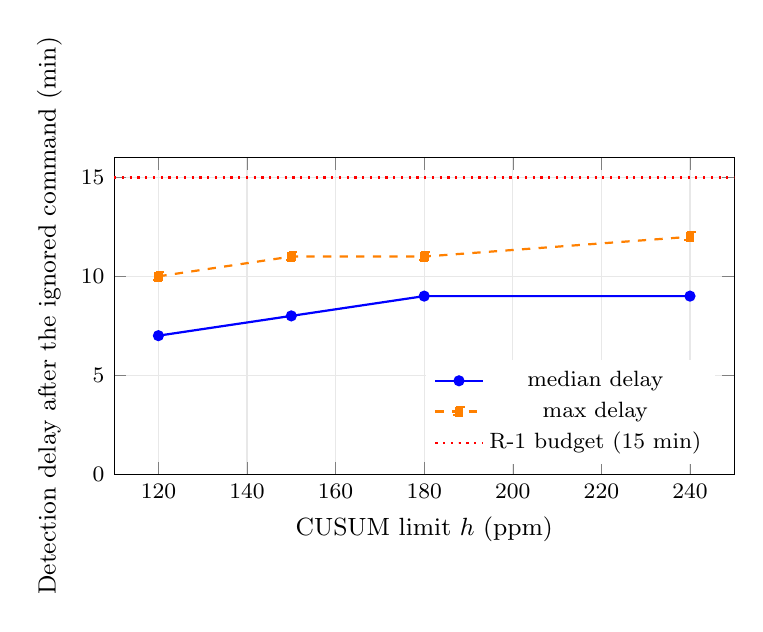
\begin{tikzpicture}
\begin{axis}[width=0.78\linewidth,height=5.6cm,
  xlabel={CUSUM limit $h$ (ppm)},ylabel={Detection delay after the ignored command (min)},
  xmin=110,xmax=250,ymin=0,ymax=16,legend pos=south east,
  legend style={font=\footnotesize,draw=none},grid=major,grid style={gray!18},
  tick label style={font=\footnotesize},label style={font=\small}]
\addplot[blue,thick,mark=*,mark size=1.6pt] coordinates {(120,7)(150,8)(180,9)(240,9)};
\addplot[orange,thick,dashed,mark=square*,mark size=1.6pt] coordinates {(120,10)(150,11)(180,11)(240,12)};
\addplot[red,dotted,thick] coordinates {(110,15)(250,15)};
\legend{median delay,max delay,R-1 budget (15 min)}
\end{axis}
\end{tikzpicture}
\end{center}
\figcap{Measured, from the spike's 20 seeds. Raising $h$ from 5σ (150 ppm) to 8σ (240 ppm) costs
about one minute of delay; lowering it to 4σ (120 ppm) already produced \textbf{1 false alarm in
20} three-hour healthy runs, while 5σ, 6σ and 8σ produced none. 150 ppm was chosen as the smallest
limit with no false alarm in the check set.}

\textbf{Two caveats bound every number above, and the spike's own result file states both.} The
observer used \emph{true occupancy}, so the healthy residual was pure sensor noise with no model
error, which makes 0 of 20 an optimistic bound. And the worst healthy seed peaked at
\textbf{149.1 ppm against $h$ = 150 ppm} (a 0.9 ppm margin, with the next-highest seed at
91.6 ppm), so the clean check set is a tail draw rather than a design property. R-3 asks the same
statistic to hold over seven days and six rooms, which is far more samples, and \textbf{the margin
did not survive that horizon}: §\ref{sec:11.2} measures \textbf{0.55} confirmed cases per fault-free week with
a \textbf{worst week of 6} against R-3's limit of one. The tuning is therefore no longer merely
reported: it is measured, and it fails. \textbf{Appendix \ref{sec:F.1}} gives both caveats in full, with
ADR-0010's attribution of why the margin was so thin; it was not the limit, which is why $k$ and $h$
are left where the spike put them rather than retuned (§\ref{sec:13.4}).
\subsection{Measured: the evaluation harness, R-1 to R-7}\label{sec:11.2}

The harness in \texttt{project/evaluation/} drives the same control and diagnosis classes the
containers run (\texttt{BuildingSimulation}, \texttt{DcvControlLoop}, \texttt{FaultMonitor},
\texttt{SupervisionService}) in one JVM against a simulated clock, with events handed between them
directly instead of through the broker and the journal replaced by a counter. One full run on
OpenJDK 25.0.3, Mac OS X on aarch64, takes 350 s of wall clock over \factExperiments{} experiments and writes nine
result tables. Every number in this subsection is read off that run, which was taken after all of
this session's changes had merged. So no figure here comes from a run of a subset of the code.

\begin{longtable}[]{@{}
  >{\raggedright\arraybackslash}p{(\columnwidth - 6\tabcolsep) * \real{0.07}}
  >{\raggedright\arraybackslash}p{(\columnwidth - 6\tabcolsep) * \real{0.09}}
  >{\raggedright\arraybackslash}p{(\columnwidth - 6\tabcolsep) * \real{0.56}}
  >{\raggedright\arraybackslash}p{(\columnwidth - 6\tabcolsep) * \real{0.28}}@{}}
\toprule
\textbf{Req.} & \textbf{Run} & \textbf{Measured} & \textbf{Verdict} \\
\midrule
\endhead
R-1 & T-24 & Stepped protocol, 20 seeds, $h$ = 150 ppm: 20/20 detected at 4 / 6 / 6 / 7 min
(min / median / p95 / max) against a 15 min budget, and p95 between 5 and 8 min over
$h$ = 50…300 ppm. Closed loop on a drawn weekday at the same $h$: 15/20 detected, 21 / 74 / 257 /
257 min & \textbf{Met as specified; not met in closed loop} \\
R-2 & T-26 & Fraction of occupied minutes at or below 1000 ppm after onset, 5 seeds. Drawn weekday
1.000, 5 of 5 seeds, unchanged with the lower CUSUM arm off and with no damper feedback. Every room
at design occupancy: 0.022 supervised against 0.009 unsupervised (\textbf{0 of 5 seeds}),
while the no-fault reference is 1.000 and 5 of 5 in every case & \textbf{Met on the case it
covers; not met at design occupancy} \\
R-3 & T-25 & Distinct confirmed cases per fault-free week over 20 simulated weeks of all six rooms:
\textbf{0.55 per week} against a limit of 1, \textbf{16 of 20 weeks clean}, worst week 6 (1.30 per
week with 9 clean weeks before ADR-0010). The scored criterion is the worst week & \textbf{Not met} \\
R-4 & T-27 & Each component killed in turn in one JVM, \textbf{23 of 23 assertions}: every
observable room \texttt{BLIND} within 4 cycles, 0 fault events while blind, 0 damper commands on
stale data, \texttt{HEALTHY} 3 cycles after readings return. \textbf{The container-level run has
since been done}: five of six rooms \texttt{BLIND} within 12 s against \texttt{docker compose},
three-cycle recovery, restart policy firing on an in-container \texttt{SIGTERM} & \textbf{Met
in-JVM and at container level} \\
R-6 & T-28 & 25\,600 zones at a p95 of about 6 s (5.68–6.05 s over five runs), inside the 60 s
interval; fitted over the nine points from 100 zones up,
p95 = $1.196\times10^{-8}\,n^{1.97}$ s with $r^2$ = 0.9991; the crossing of 60 s extrapolated at
$\approx$ 86\,000 zones; saturated element \texttt{AhuFlowModel.believedFlowTo}, $\Theta(n^2)$ per
cycle. \textbf{The deployed ceiling is a different and far smaller number}: 58 zones, bounded by
BuildSim's floorplan rather than by the monitor & \textbf{Met in the harness}, and the two ceilings
are never quoted as one \\
R-7 & T-34b & Injected room rotated over all six rooms, 3 seeds, 3 configurations, in \emph{two
occupancy regimes}, 540 observed rooms. Drawn weekday, 270 rooms: \textbf{0 failed}, airflow inside
the 5 \% tolerance everywhere. Design occupancy, 270 rooms: \textbf{231 failed} (215 accused of a
fault they did not have, 16 more outside the airflow band at a worst 0.058919, the two sets
disjoint); 40 rooms reached \texttt{COMPENSATING} and \textbf{130 of the 215 falsely latched rooms
reached \texttt{DEGRADED}}. The supervisor does not merely accuse those rooms, it takes their
dampers off the inner loop & \textbf{Met on the drawn weekday; not met at design occupancy} \\
\bottomrule
\end{longtable}
Six of the seven requirements are scored in that table; \textbf{R-5's evidence is a live rebuild
rather than a harness experiment}, reported with the journal in §\ref{sec:5} and in Appendix \ref{sec:G}.

\textbf{Two readings of the table matter more than any single row.} The first is that \textbf{every
failing verdict above is a regime statement, not a global one}: R-1 is met on the stepped protocol
its own verification column names and fails in closed loop; R-2 is met on the drawn weekday and
fails with every room at design occupancy; R-7 is met on 270 drawn-weekday observed rooms and fails
on 231 of 270 at design occupancy. Quoting either arm without the other misrepresents the result, so
this report never does. The second is that \textbf{R-3 is not one failing requirement among four; it
is the one whose failure the other three inherit.} R-2's design-occupancy seeds fail partly because
false alarms have already latched rooms that would otherwise have been healthy dampers to trim
(R-3's false alarms consume the lever R-2 depends on), and the larger half of R-7's failure is 215
observed rooms accused of a fault they did not have, which is R-3's rate arriving inside another
requirement's experiment in a regime R-3's own replay never visits.

\textbf{Appendix \ref{sec:F.3} carries the working behind every verdict}: what separates protocol from
occupancy in R-1's two arms, the stratification of T-24's 20 drawn weekdays, T-25's baseline contest
and T-29's learned contender with the operating point attached to each ratio, R-2's five seeds and
the lever each plan ran out of, R-3's 26 pre-fix confirmations classified by arm and cause with the
half of the fix that was declined on evidence, R-6's fit and its two ceilings, and R-7's two
disjoint failing clauses with the supervisor-dead pass that separates them.

\subsection{Proved: compensation holds the healthy rooms exactly}\label{sec:11.3}

This result is analytic and pinned by unit tests, not produced by an experiment, and it is
presented as such. The per-room flows below follow from Section \ref{sec:7.4}'s closed form at Section \ref{sec:6}'s
parameters: five healthy dampers at 0.60, A145's frozen at 0.15, baseline fan 0.70, trim
$t = 0.360$, fan raised to $s = 0.880$.

\begin{center}
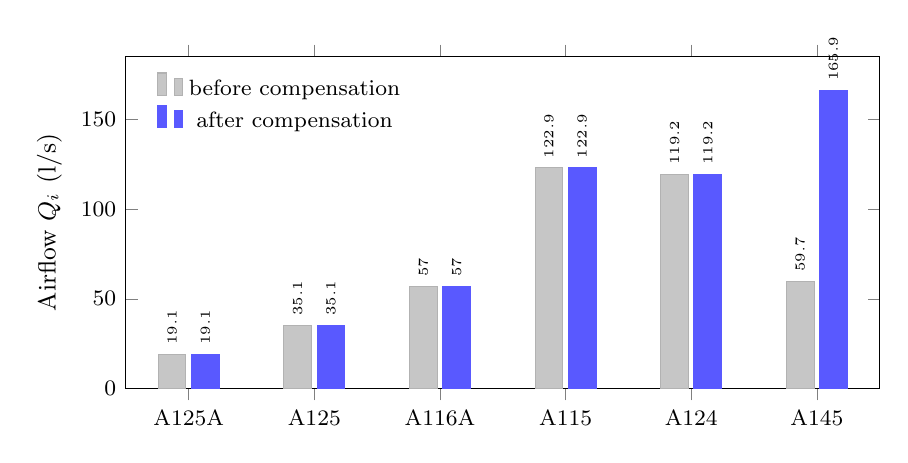
\begin{tikzpicture}
\begin{axis}[width=0.92\linewidth,height=5.8cm,ybar,bar width=10pt,
  ylabel={Airflow $Q_i$ (l/s)},ymin=0,ymax=185,
  symbolic x coords={A125A,A125,A116A,A115,A124,A145},xtick=data,
  legend pos=north west,legend style={font=\footnotesize,draw=none},
  nodes near coords,every node near coord/.append style={font=\tiny,rotate=90,anchor=west},
  enlarge x limits=0.10,tick label style={font=\footnotesize},label style={font=\small}]
\addplot[fill=gray!45,draw=gray!60] coordinates {(A125A,19.1)(A125,35.1)(A116A,57.0)(A115,122.9)(A124,119.2)(A145,59.7)};
\addplot[fill=blue!65,draw=blue!65] coordinates {(A125A,19.1)(A125,35.1)(A116A,57.0)(A115,122.9)(A124,119.2)(A145,165.9)};
\legend{before compensation,after compensation}
\end{axis}
\end{tikzpicture}
\end{center}
\figcap{Computed from the solver's closed form, and asserted by
\texttt{CompensationSolverTest}. A145, frozen at its 0.15 damper floor, goes from 59.7 l/s to
165.9 l/s (its full design flow, a gain of 2.78), while the five healthy rooms' flows are
unchanged to within $10^{-15}$. This is arithmetic that closes exactly, not a measurement; the
closed-loop CO₂ that is R-2's actual criterion is measured separately, and §\ref{sec:11.2} reports where it
holds and where it does not.}

\begin{longtable}[]{@{}
  >{\raggedright\arraybackslash}p{(\columnwidth - 6\tabcolsep) * \real{0.2870}}
  >{\raggedright\arraybackslash}p{(\columnwidth - 6\tabcolsep) * \real{0.1722}}
  >{\raggedright\arraybackslash}p{(\columnwidth - 6\tabcolsep) * \real{0.1722}}
  >{\raggedright\arraybackslash}p{(\columnwidth - 6\tabcolsep) * \real{0.3636}}@{}}
\toprule
\textbf{Case} & \textbf{Trim $t$} & \textbf{Gain achieved} & \textbf{Healthy flow deviation} \\
\midrule
\endhead
Requested gain 2.0, fan at 0.70 & 0.500 & exactly 2.000 & \textbf{0}, fan raised to 0.8012 \\
Restore A145 to design flow, fan at 0.70 & 0.360 & 2.779 & \textbf{0}, fan raised to 0.880 \\
Requested gain 4.0, fan \emph{already} at 1.00 & 0.733 & \textbf{1.296 only} & exactly 5 \%, the
stated tolerance; the fan has nothing left to raise \\
Damper stuck fully shut & no trim & \textbf{none} & no command issued; critical work order instead
\\
\bottomrule
\end{longtable}

The third row is the honest one and the most useful: with the fan already saturated (peak
occupancy, or a blocked filter the inner loop has already answered with speed), compensation
delivers a gain of \textbf{1.296, not 4}, and buys even that by taking exactly 5 \% from each
healthy room. Flow is redistributed, not created. Reporting R-2 without that bound, and without the
stuck-shut bound, would misrepresent it: the claim this design supports is not ``the system keeps
faulted rooms breathable'' but ``it does so while the damper still passes 15 \% of its design
opening and the fan has headroom''.

\subsection{Proved: architectural properties}\label{sec:11.4}

These are properties of code rather than of physics, and a simulator is the right instrument for
them. Each is covered by unit tests in the control and entity layers: that
\texttt{fault-monitor} never writes an actuator topic; that an aggregate cannot be constructed in
an illegal state (a \texttt{FanSpeed} outside $[0.2, 1.0]$, a damper position outside $[0,1]$);
that a latched \texttt{FaultCase} leaves \texttt{CONFIRMED}/\texttt{COMPENSATING} only through
\texttt{serviced()}; that \texttt{BLIND} has no edge into an open case; and that a zone in
\texttt{DEGRADED} mode receives no normal control command.

\subsection{Not measured: what the numbers above do not say}\label{sec:11.5}

The detector is evaluated against its own generator. \texttt{physics-simulator} freezes a damper,
scales flow by $(1-\beta)$ or adds a sensor offset, and \texttt{fault-monitor} looks for exactly
those three things using the same mass balance and the same flow split. \textbf{Every detection
result is therefore a measurement of self-consistency between two pieces of one person's
arithmetic.} The p95 delay (R-1), the false-alarm rate (R-3) and the comfort percentile (R-2) are
conditional on the generator: they describe how this detector behaves against this fault
definition, and say nothing about a real air handler. Section \ref{sec:13.2} develops this.

A second, sharper limit on what can be claimed, and T-15 has since made it sharper still: of the
faults the project set out to name, \textbf{one is classified and the others can only be pointed at}.
\texttt{STUCK\_DAMPER} is the reliable one, and T-24, T-25, T-26 and T-34b are all measurements of
it. \texttt{BLOCKED\_FILTER}'s branch is \textbf{unreachable with this physics} for structural
reasons §\ref{sec:13.1} sets out: it confirms as \texttt{UNCLASSIFIED} with its plant power excess reported,
which is the right behaviour for a case the system cannot prove. And \texttt{SENSOR\_DRIFT} is
\textbf{never emitted at all} (0 of 76 runs from a drift ramp and 0 of 76 from a step offset),
so the room is named a stuck damper instead: a confident, specific, wrong work order rather than an
honest \texttt{UNCLASSIFIED}. \textbf{Appendix \ref{sec:D.3}} records why that is a property of the classifier
rather than of the generator, an attribution this report had the wrong way round until the experiment
was run.

\subsection{Every pending measurement, in one place}\label{sec:11.6}

\textbf{Every row of that register is now filled, and no row is filled with an estimate.} What was a
fourteen-row table of pending measurements is seven rows of experiments that have all run: T-24's
occupancy stratification, T-20's live case rebuild, T-27's container kills, T-15's confusion matrix
over 218 runs, T-29's optional learned contender (\textbf{measured and dropped}), T-23's
dashboard frames, and T-35's reordering of the diagnosis (\textbf{measured and not adopted}). Each
row keeps the bound on what its evidence actually is.

\textbf{The table being full is not the same as every requirement passing}: R-1 and R-3 still fail on
the arms §\ref{sec:11.2} names, R-2 and R-7 fail on the harder of their two occupancy regimes, and one of four
injected mechanisms is classified. \textbf{Appendix \ref{sec:G}} is the register row by row, with one result the
obvious experiment measures wrongly: a \texttt{docker kill} cannot tell a working restart policy
from a missing one, because the daemon records it as a manual stop.

\subsection{Measured: what the compensation costs in energy}\label{sec:11.7}

This is the last measurement folded in, which is why it sits after the register rather than among
its siblings. It needed no new experiment: both halves are columns of
\texttt{evaluation/results/T-26-comfort.csv}, the same five-seed run §\ref{sec:11.2} scores R-2 from, read
together for the first time.

Fan power follows the affinity law, $P \propto s^3$ (§\ref{sec:6}, Appendix \ref{sec:E}), so the second lever is priced
superlinearly while the airflow it buys is not. The question that makes it a sustainability result
rather than an arithmetic one is what the system actually spent, per regime, against what the
spending bought.

\begin{longtable}[]{@{}
  >{\raggedright\arraybackslash}p{(\columnwidth - 8\tabcolsep) * \real{0.26}}
  >{\raggedright\arraybackslash}p{(\columnwidth - 8\tabcolsep) * \real{0.17}}
  >{\raggedright\arraybackslash}p{(\columnwidth - 8\tabcolsep) * \real{0.19}}
  >{\raggedright\arraybackslash}p{(\columnwidth - 8\tabcolsep) * \real{0.19}}
  >{\raggedright\arraybackslash}p{(\columnwidth - 8\tabcolsep) * \real{0.19}}@{}}
\toprule
\textbf{Regime} & \textbf{Comfort, no supervisor} & \textbf{Comfort, supervisor} & \textbf{Mean
plan fan speed} & \textbf{Fan power vs normal} \\
\midrule
\endhead
Drawn weekday & 1.0000 & 1.0000 & \textbf{0.7000} & \textbf{×1.00} \\
Design occupancy & 0.0094 & 0.0217 & 0.8171 (max 1.0000) & \textbf{×1.59} (max ×2.92) \\
\bottomrule
\end{longtable}

\textbf{The result is the shape of those two rows, not either number on its own.} On the drawn
weekday, the regime where R-2 is met, the plan's fan speed is \textbf{0.7000 in all five
seeds}: the common trim on the healthy dampers covers the whole requested gain and \emph{the raise
is never spent at all}. Compensation there is free. At design occupancy it costs on average
\textbf{1.59 times the fan power}, and up to 2.92 times where no healthy room is left to
over-supply, to move occupied comfort minutes from 0.0094 to 0.0217: a gain of
\textbf{0.0123 against an acceptance criterion of 0.95}.

So the energy is spent almost exactly where it does least good, and that is a property of the
\emph{plant}, not of the control law. The ceiling is the damper floor and the fan curve: when every
room is generating CO\textsubscript{2} at design rate, there is no healthy room with spare airflow
to trim, the solver falls back on the one lever that remains, and that lever is the cubed one.
\textbf{Buying 1.2 \% of comfort minutes for 59 \% more fan energy is not a trade worth making},
and the honest conclusion is that at design occupancy the supervisor should \emph{decline} to
compensate and say so in the work order, which is what the stuck-shut case already does, where
the plan reports ``no air path'' and the narrative turns to occupancy advice (§\ref{sec:7.4}, Appendix \ref{sec:E})
rather than spending the fan on a room it cannot reach.

That change is not made here. It would alter R-2's measured arm two days before this document was
frozen, and a requirement that fails for a mechanism this report can name is better evidence than
one that passes because the experiment was changed after the result was known. It is recorded in
§\ref{sec:13} as the first thing to do next, with the number that justifies it.

\section{Dashboard}\label{sec:12}

The operator view has two halves, deliberately.

\textbf{On BuildSim's own viewer}, \texttt{dashboard} repaints all four layers every 5 s, and a
query parameter switches which one the rooms are coloured by. The viewer offers a 3D mode and a
floor plan; \textbf{every capture in this report is the plan}, deliberately. It shows all six
rooms and which one has gone red in a single frame, where a perspective render hides whichever
rooms are behind the near wall. The layer being painted is the same either way: the colouring is
\texttt{dashboard}'s, pushed through BuildSim's room-layer API, and the view toggle is the
operator's.

\begin{longtable}[]{@{}
  >{\raggedright\arraybackslash}p{(\columnwidth - 6\tabcolsep) * \real{0.15}}
  >{\raggedright\arraybackslash}p{(\columnwidth - 6\tabcolsep) * \real{0.14}}
  >{\raggedright\arraybackslash}p{(\columnwidth - 6\tabcolsep) * \real{0.26}}
  >{\raggedright\arraybackslash}p{(\columnwidth - 6\tabcolsep) * \real{0.45}}@{}}
\toprule
\textbf{Layer} & \textbf{Range} & \textbf{Why that range} & \textbf{What it shows the operator} \\
\midrule
\endhead
\texttt{co2} & 420–1500 ppm & Outdoor level to half again the comfort limit & The air, which is what
occupants feel\\*
\texttt{residual} & $-100$ to $+500$ ppm & The spike measured healthy residuals spanning $-76.5$ to
$+80.3$ ppm and a stuck damper's post-command mean at 507.8 ppm, so the scale is set by measurement
rather than by taste & How far the room is from what its command owed\\*
\texttt{cusum} & 0–300 ppm & Twice $h$, so the limit sits at mid-scale & How close the room is to
confirmation\\*
\texttt{state} & 0–3 & latched 3, stale or \texttt{BLIND} 2, \texttt{SUSPECT} 1, else 0 & The
equipment, which is not the same thing as the air \\
\bottomrule
\end{longtable}

The \texttt{state} layer is the interesting one and it exists for one reason: \textbf{it keeps a
latched room hot after compensation has pulled its residual back to zero.} On the \texttt{co2} and
\texttt{residual} layers a compensated room looks healthy (which is true of the air and false of
the equipment), and the severity ordering is chosen precisely so that the latched room stays the
hottest thing on the floor. The same concern shapes the projection behind the view: only an explicit
fault-state event moves a room's monitor state, so the arrival of small residuals, which is exactly
what successful compensation produces, cannot talk the display out of a diagnosis the monitor
latched.

A stale measurement is painted at the layer minimum rather than frozen at its last value, because
BuildSim's layer API carries numbers and a range with no no-data sentinel; \texttt{state} is exempt
because it is not a measurement. And \texttt{dashboard} \textbf{never writes a BuildSim alert}:
alerts are a whole-collection PUT, so a second writer would erase the supervisor's work orders
rather than add to them. One writer per resource, for the same reason one component commands.

\textbf{Beside it}, a server-rendered HTML table at port 8080 (no JavaScript, no framework, no
CDN, just a meta refresh every 5 s) with \texttt{GET /api/state} serving the same view as JSON and
\texttt{GET /api/cases/\{caseId\}} replaying one diagnosis out of the journal, which is R-5's
interface and not a convenience. The replay is encoded with the same codec that published the
events, so a replay cannot disagree with what went over the wire, and its failure modes are
distinguished rather than collapsed: 400 for a blank id, 404 for an unknown case, and 503 with
\emph{different detail text} depending on whether the journal is unconfigured or configured but
unreachable.

Every dependency of this page is optional, and that is a deliberate inversion of the usual
dependency direction for a dashboard: it keeps serving when the broker, BuildSim or the database is
down, retrying each on its 5 s tick, which makes it the instrument for telling whether the rest of
the system is alive. Its health probe is never reported DOWN for the same reason: a dashboard that
failed readiness because no readings were arriving would be restarted by the orchestrator at
precisely the moment an operator needed to look at it. The price is a little duplicated
state-handling and a page that can show a confidently empty table.

\begin{center}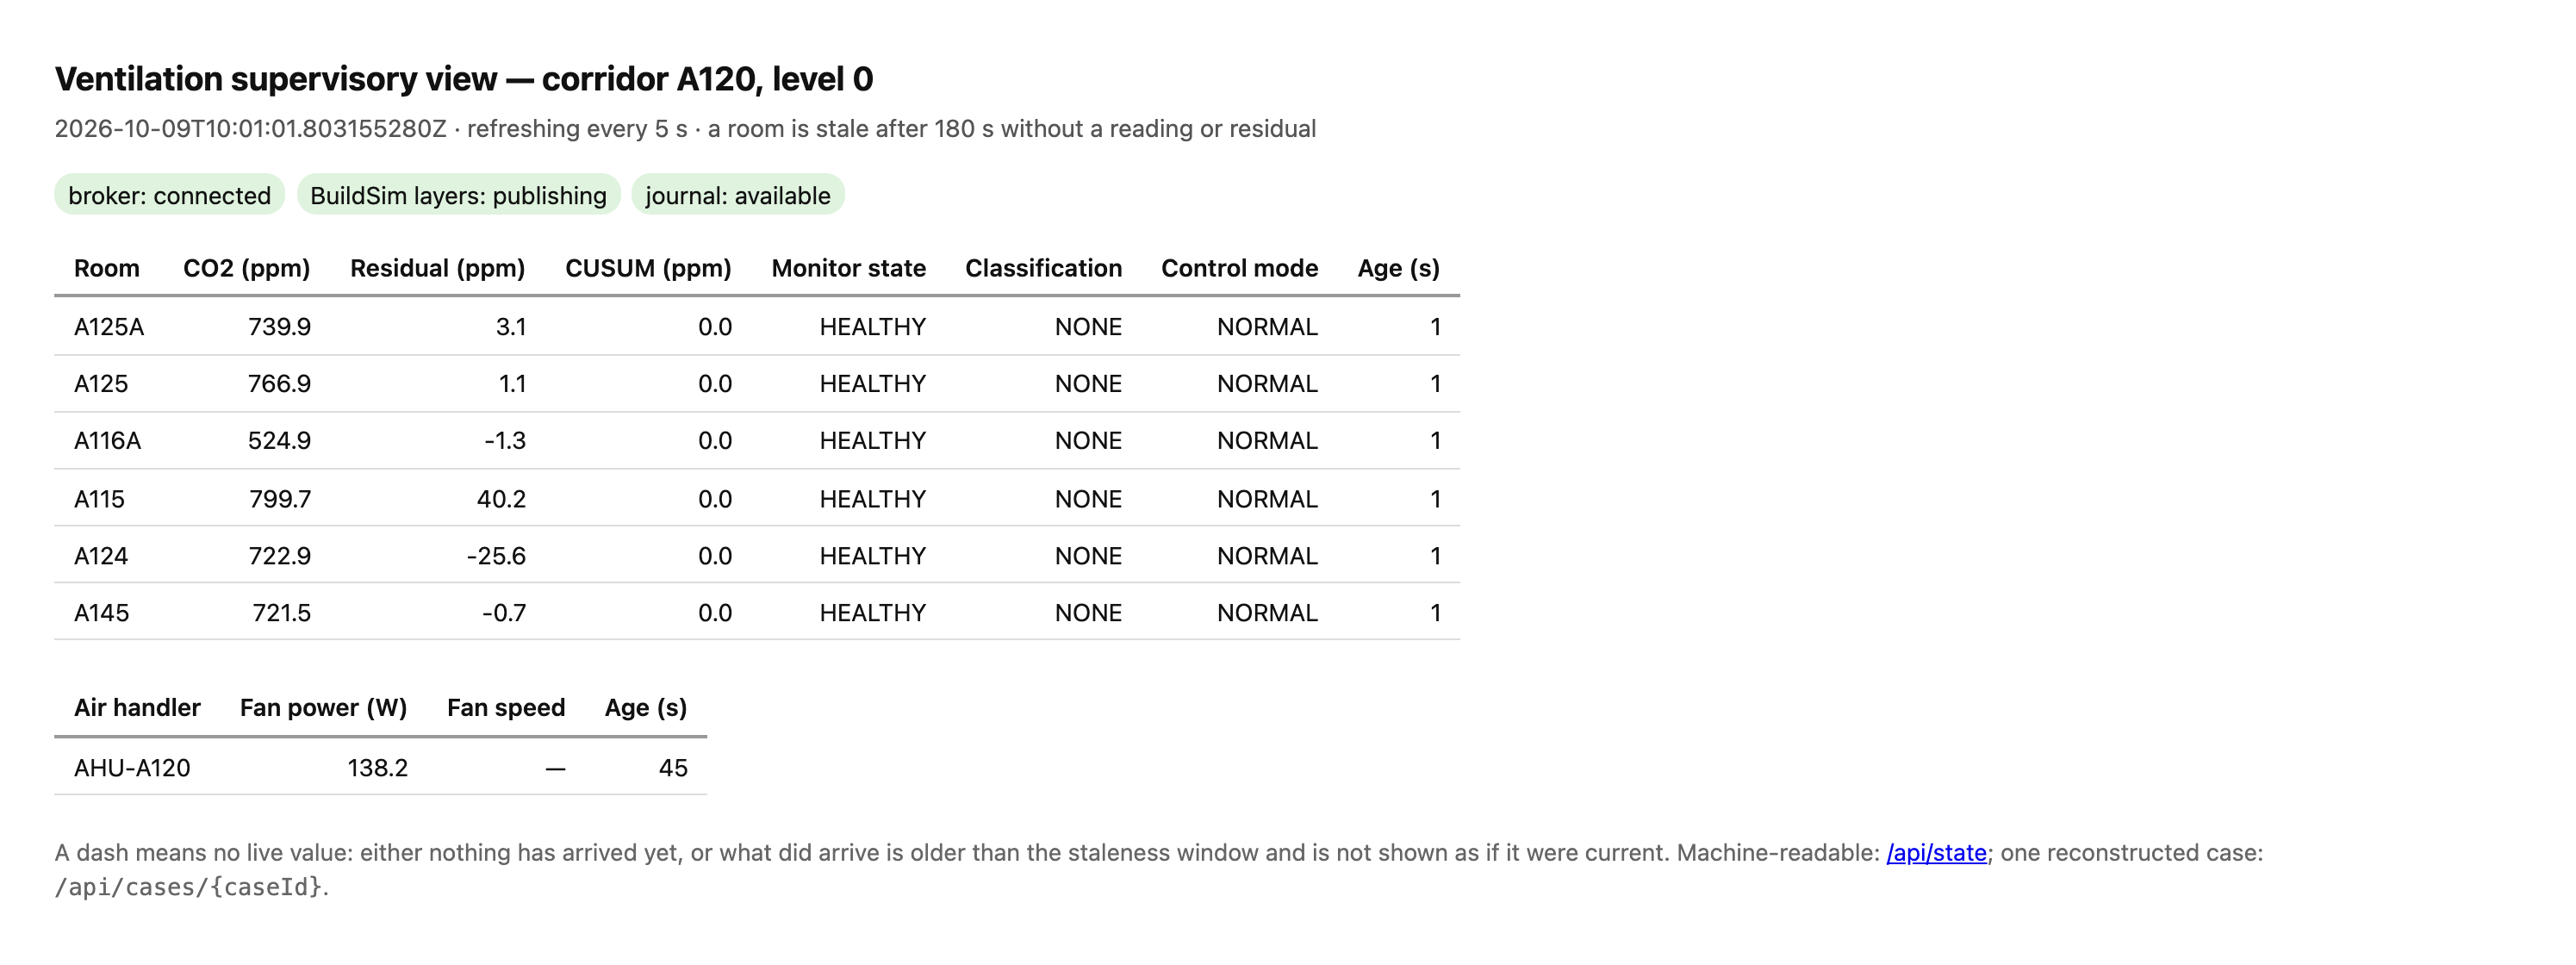
\includegraphics[width=\linewidth]{screenshots/dashboard-not-firing.png}\end{center}
\figcap{Simulated 10:01:01, 46 simulated minutes after the damper jammed. A115 has climbed to
799.7~ppm and its residual is \textbf{+40.2~ppm}, while its CUSUM is still \textbf{exactly 0.0}
and every room reads \texttt{HEALTHY}. This is the frame worth defending against ``your detector
is only a threshold'': a threshold placed anywhere below 40~ppm would have fired here. The CUSUM
has not accumulated because it is not driven by this column: \texttt{ZoneMonitor} advances it
on the \emph{occupancy-plausible} residual, measured minus the prediction's \emph{ceiling}, so the
table's residual and the detector's input are two different series (§\ref{sec:11}, ADR-0010). The fan speed
shows an em-dash because no live value had arrived yet, which is the no-stale-number rule in
Section \ref{sec:12} acting rather than a gap.}

Three further frames are in \textbf{Appendix \ref{sec:H.1}}: the same table with A115 \texttt{CONFIRMED} at
simulated 10:23:27, with the other five rooms \texttt{HEALTHY} at CUSUM 0.0, R-7's isolation
visible in one frame; BuildSim's own floor plan
beside the work order the \emph{supervisor} PUT, naming the diagnosis, the action taken and the bound
the plan ran into; and corridor A120 painted by all four layers at one instant with A115 latched and
\texttt{COMPENSATING}. That last figure is this section's argument measured rather than asserted:
compensation has done its job, so on \texttt{co2} the broken room is the second coolest on the floor
and on \texttt{cusum} it is indistinguishable from five healthy rooms, and only \texttt{state} still
says the equipment is broken.

What the figures do \emph{not} settle is what the view \emph{must} show: no requirement states it,
so these are evidence that the operator path works end to end, not evidence against a criterion.

\subsection{Two defects the capture found, and one limit it exposed}\label{sec:12.1}

Capturing those frames found two defects and exposed one limit, and \textbf{Appendix \ref{sec:H.2}} reports all
three in full. \textbf{The layers were overwriting each other}: \texttt{/api/room-layers} is a
collection endpoint whose PUT replaces the whole collection, and the dashboard was publishing its
four layers one at a time, so each call erased the one before it and only the last layer of the enum
ever reached BuildSim, with every individual PUT returning 200, so nothing anywhere said so. The
fix sends every layer on every call, and the run above confirms it against the real stack:
\texttt{GET /api/room-layers} returns \textbf{four layers of six zones each}. \textbf{A compensated
room is painted exactly like a dead sensor}, because $-100$ is both the bottom of the
\texttt{residual} scale and the only no-data encoding BuildSim's layer API offers; that is recorded
as a limit rather than patched, for a reason the appendix gives. And \textbf{\texttt{SUSPECT} cannot
be photographed}: a 1~Hz poll of \texttt{/api/state} caught A115 in it in \textbf{2 of 295 usable
samples} against a page that refreshes every 5~s, so that state is evidenced from the
\texttt{decisions} journal and from the poller instead, and the screenshots are taken only at states
that latch.

\section{Risks and critical reflection}\label{sec:13}

This section is the honest account, and it is deliberately the least flattering part of the
document. Several of the findings below are not disclosures but \emph{functional holes} (things
that do not work, rather than things that are merely unvalidated), and they are stated first
because they are the ones worth the most to find.

\subsection{Four functional holes, two of which are now closed}\label{sec:13.1}

Four holes, each with its verdict; \textbf{Appendix \ref{sec:I.1}} carries the mechanism behind every one.

\textbf{1. A damper stuck \emph{wide open} is invisible at the deployed setting.} The statistic is
two-sided, and the deployed \emph{guarded} lower arm catches the low-side fault with a safety
consequence: a sensor drifting downward, which under-ventilates an occupied room and betrays
itself by reading below the 420 ppm outdoor level. It cannot catch a damper stuck open, because
``everybody left the room'' explains a room that stopped getting stuffier at least as well and
nothing inside a ten-minute judging window separates them. The unguarded arm sees both and costs more
false confirmations than R-3 allows. \textbf{An observer with no occupancy signal cannot have both,
and the choice was made in R-3's favour.}

\textbf{2. \texttt{serviced()} had no transport, and now it has one. Closed.} The only exit from a
latched case was unreachable in deployment, so a false latch was \textbf{permanent}.
\texttt{ServiceReported} now travels on \texttt{service/\{zone\}} validated against the open case,
and the dashboard exposes
\texttt{POST /api/zones/\allowbreak \{zone\}/cases/\allowbreak \{caseId\}/serviced}. The whole
\texttt{CONFIRMED} → \texttt{COMPENSATING} → \texttt{SERVICED} → \texttt{WARMUP} →
\texttt{HEALTHY} lifecycle is tested end to end. This matters most to §\ref{sec:13.8}, whose argument is that a false positive
costs one technician visit, an argument that was being made against a system where it cost that
visit \emph{and} a permanently wrong work order.

\textbf{3. The ambiguous fault is absent from the model, so the classifier's hardest discrimination
is never tested.} The ambiguity a real building would produce (a partial obstruction in one duct
branch, reading as both a partly stuck damper and a partly blocked filter) \textbf{is not in the
fault model at all}, and the enumeration cannot express it, so a clean confusion matrix would have
been weak evidence rather than strong.

\textbf{4. And worse than untested: the \texttt{BLOCKED\_FILTER} branch is unreachable with this
physics.} This is the finding I least expected and would lead with in the oral; a unit test pins the
outcome as \texttt{UNCLASSIFIED} so it cannot rot. Two structural reasons, neither a bug to patch:
the proportional split only redistributes a fixed total, so no command the observer judges moves all
six residuals the same way; and the quasi-steady generation estimate absorbs the blockage exactly.
True flow low by $(1-\beta)$, believed flow high by the same factor, so only the time constant
differs. The work order still carries the measured plant power excess, which is right for a case the
system cannot prove and is not a working three-way classifier. \textbf{Of the mechanisms this project
set out to name, exactly one is classified: \texttt{STUCK\_DAMPER}}. \texttt{BLOCKED\_FILTER} can
be pointed at but never confirmed, and \texttt{SENSOR\_DRIFT} is never emitted at all, 0 of 76 runs
from a drift ramp and 0 of 76 from a step offset (§\ref{sec:7.3}, §\ref{sec:11.5}).

\subsection{The detector is evaluated against its own generator}\label{sec:13.2}

The simulator produces exactly the faults the monitor looks for, using the same mass balance and the
same flow split. That invalidates the \textbf{detection-performance numbers as transferable
quantities} (R-1's delay, R-3's false-alarm rate and R-2's comfort percentile are conditional on my
own fault definition) and does \emph{not} invalidate the \textbf{architectural claims}, which are
properties of code: that the monitor never commands, that a latched case has one exit, that stale
readings give \texttt{BLIND} with zero fault events, that a confirmed fault changes strategy without
stopping ventilation. A simulator is the right instrument for those, as it is for R-5 and R-6. Closing
the gap needs measured fault data from a real air handler with service records, or at minimum a second
fault model written independently of the detector. Neither was in scope, and the gap is no smaller for
that.

\subsection{Every physical parameter is invented}\label{sec:13.3}

The full list, so it can be judged rather than taken on trust: the 3 m ceiling, from which every
volume is \texttt{area} $\times$ 3.0; the opening law $a_i = p_i A_i$ with authority proportional to
design flow, and the proportional split; $Q_\text{nom}$ = 0.59 m³/s; $P_\text{nom}$ = 400 W from an
assumed 400 Pa at 0.6 efficiency; \texttt{minimumDamperPosition} = 0.15; the \textbf{affinity
exponent 3}, asserted rather than derived; $\beta$, which has no design value at all and is only a
fault-injection magnitude; drift as an uncapped linear ppm/hour ramp; and the whole occupancy
schedule.

Which of them matter, and how, is the useful part. \textbf{First-order on R-1}: ceiling height,
because every time constant is $V/Q$ and $V$ is linear in it, so a 2.7 m ceiling makes all six rooms
10 \% faster; the design-flow rule, because the observer recovers design occupancy from the
authority and drives suspicion against that ceiling; and the schedule, because a room empty most of
the day hides its own fault. \textbf{First-order on R-2}: \texttt{minimumDamperPosition} and a
sizing that leaves $413/411.4 \approx 1.004$ at the normal speed and 43 \% up to $s=1$, which
together decide whether compensation has anything to work with. \textbf{Near-cosmetic}: $P_\text{nom}$, because the classifier tests a \emph{ratio}
against the affinity-law prediction, so 400 W cancels. \textbf{Worse than cosmetic}: the exponent
3, because the generator and the detector share it, so the blocked-filter power test cannot fail
except through $\beta$. Removing this gap needs a commissioning report: a measured fan curve, a
measured pressure drop, a people counter.

One of them was corrected on measurement rather than argued, and it belongs here because the first
choice was wrong. $Q_\text{nom}$ was initially the design total rounded up, which meets the
simultaneous design condition only at $s=1$, the one speed compensation needs to borrow from. Run
at the normal 0.7 that plant delivers 294 l/s against a 411.4 l/s design total, and the consequence
was not subtle: with \textbf{nothing broken} no room could be held below 1000 ppm at design occupancy
and the monitor confirmed a fault in all six, because a uniformly starved building looks exactly like
a faulty one. Sizing from $\Sigma$ design $\div\ 0.7$ separates the two jobs the rating was doing at
once. \textbf{The fix is not free, and this is the honest cost: margin masks faults.}
\textbf{Appendix \ref{sec:I.2}} gives the correction, its measured price (a filter blocking 35 \% no longer
starves the rooms enough for the monitor to confirm it) and the no-fault arm that now holds every
occupied minute at or below 1000 ppm at design occupancy on all five seeds, which is the figure the
earlier sizing scored 0.000 on.
\subsection{The CUSUM margin is thin, R-3 does fail, and the margin was the symptom rather
than the cause}\label{sec:13.4}
The worst healthy seed peaked at 149.1 ppm against $h$ = 150 ppm at $\sigma$ = 30 ppm, over three
hours in one room: a \textbf{0.9 ppm margin}, with the next seed at 91.6 ppm, so it is a tail draw and
not a design property. R-3 asks for the same statistic across six rooms over seven days, far more
samples, and the measurement contradicts the analytic run length: over 20 fault-free simulated weeks
of all six rooms the monitor raises \textbf{0.55 confirmed cases per week against R-3's limit of one},
with \textbf{16 of 20 weeks clean} and a worst week of 6, against 1.30 per week and 9 clean weeks
before ADR-0010, while on the same tuning R-1's stepped p95 is 6 min against a 15 min budget
(§\ref{sec:11.2}). The scored criterion is the worst week, so R-3 fails.

\textbf{But $h$ was never the knob}, and that is the correction this section needs. ADR-0010
attributed the failure to the \emph{reference} the limit is applied to rather than to the limit: both
plausibility guards were being corrected 30 \% of the way onto every reading, so each CUSUM arm was
accumulating a filter error instead of a residual. Correcting the lower arm's half of it halved the
rate with $k$ = 30 ppm and $h$ = 150 ppm \emph{untouched}. So $k$ and $h$ stay where the spike put
them rather than being retuned until R-3 passes: retuning a limit on the experiment that failed it
is the same methodological error §\ref{sec:13.10} names. The upper arm's half of the same defect is measured,
meets R-3 outright, and was declined because it costs three other requirements (§\ref{sec:11.2}, ADR-0010).
\textbf{Appendix \ref{sec:I.3}} gives the full argument, including which week and which arm the residual
failures sit on.

\subsection{R-7 fails at design occupancy, and the failure is R-3's arriving somewhere else}\label{sec:13.5}

Until this revision R-7 was reported as met, full stop, on 270 observed rooms. It was met on the
occupancy regime it had been run in. With every room at its design head count the same experiment
fails \textbf{231 of 270}, and the shape of the failure is the result.

The two failing clauses are \textbf{disjoint}: 215 observed rooms were themselves \emph{accused of a
fault they did not have} and 16 more sat outside the 5 \% airflow band at a worst deviation of
0.058919 (215 plus 16 is the 231), and they attribute in opposite directions, which the
supervisor-dead pass shows. Accusations run 85 of 90 rooms with the supervisor \emph{dead} against
130 of 180 with it live, so they belong to the regime and the monitor rather than to the response to
the fault; airflow breaches run 0 of 90 dead against 16 of 180 live, so that half is the
compensation's own cost and nothing else's.

\textbf{And the accusation is not where it stops.} Of those 215 falsely latched rooms,
\textbf{130 were also taken off the inner loop}: the supervisor published \texttt{DEGRADED} for
them, confiscating the damper of a room with nothing wrong with it. Zero rooms were degraded without
first being latched, so every one of the 130 is downstream of a false confirmation rather than a
separate defect. That figure reads 0 in any copy of \texttt{T-34b-room-isolation.csv} generated
before the supervisor began re-asserting a degraded zone's mode on every cycle; the confiscation was
always happening, and what changed is that it is now announced often enough to be seen.

\textbf{So the larger half of R-7's design-occupancy failure is R-3's false-alarm rate, measured by a
different experiment in a regime R-3's own replay never visits.} That is the second time this report
has had to say it (§\ref{sec:11.2} records the same pattern inside R-2), and \textbf{R-3 is not one failing
requirement among four; it is the one whose failure the other three inherit}. ADR-0009 predicted this
collision and noted that no experiment asserted R-7 in that regime. One does now. Two bounds travel
with the finding and \textbf{Appendix \ref{sec:I.4}} states both: one of the two airflow columns cannot falsify
this requirement at all, and the 5 \% bound's \emph{reference plant} is ambiguous in a way ADR-0008
never settles (an ADR-level question, not a code change).

\textbf{The mechanism that turns one false alarm into six, which this section owed the reader and
until now left in Appendix \ref{sec:F}.} A false \texttt{STUCK\_DAMPER} does not merely add one accusation;
it \emph{pins} that room's believed opening in \texttt{AhuFlowModel}, and the proportional split is
a ratio over all six rooms. Pin one denominator term and the other five rooms are credited with air
they are not receiving, so their predicted concentrations fall below their readings and they confirm
in turn. When the false-alarm rate was 1.30 per week, instrumenting the replay by room, hour, arm
and whether any room was already pinned showed the two halves to be \textbf{exactly even: 13 of the
26 confirmations were raised with no room yet pinned, and 13 were raised while another already
was}. And of the 17 upper-arm confirmations, 11 were cascaded. One seed latched four rooms in
53 minutes; another latched all six (ADR-0010, Appendix \ref{sec:F}).

\textbf{This is the finding that makes R-3 structural rather than statistical}, and it is why
ADR-0010's response was a re-anchor rather than a larger $h$: a confirmation that pins a damper now
re-anchors the other five rooms and resets their arms, because a step change in believed airflow
makes every ppm banked before it a statement about a different building. Aiming at the cascaded half
took the rate from 1.30 to 0.55 and the clean weeks from 9 to 16 while moving no other requirement.
The half that remains is the primary half, which no re-anchor can reach: \textbf{a shared-plant
design couples its own false alarms, and that coupling is a consequence of ADR-0008's option B
rather than a defect in the detector}. Independent rooms would not cascade, and would also have made
R-7 hold by construction and its experiment measure nothing (§\ref{sec:4.7}).

\subsection{The third diagnostic signal is blind after a confirmation, and reordering the
pipeline does not help}\label{sec:13.6}
§\ref{sec:7.3} records that the stuck-damper leaf fires on two signals rather than three, because a probe can
only be requested once a case is latched and no step has been judged at classification time. The
obvious repair is to reorder: latch as usual, withhold the diagnosis, ask for the probe immediately,
and name the fault when the step lands. \textbf{It was built, measured over 176 paired runs on
identical seeds, and not kept.} It does what it was designed to do (detection moves in 0 of 88
pairs and the fault is named on a genuinely judged step in 28 of the 39 runs that defer, against none
before), and \textbf{the settled classification is identical in all 88 pairs}, because the judged
step reads \texttt{MISSING} for a stuck damper, a blocked filter, nine rooms whose dampers are in
perfect health, and the run with nothing injected. A signal that reads the same for every condition
decides nothing.

The cause is a located defect older than the ordering, and \textbf{correcting that baseline makes the
reorder worse rather than better}, which is the finding worth defending, because by the time a
probe can be commanded the supervisor has degraded the zone, raised the fan and trimmed the other
five, so the room's answer is mostly the compensation's. \textbf{Appendix \ref{sec:I.5}} carries the defect, the
counterfactual and the conclusion, which is the one concrete thing this report would hand to a
successor: \textbf{a three-signal stuck-damper diagnosis needs a step judged \emph{before} a case
opens} (the inner loop's own trims, read against a baseline that survives them) rather than a
probe requested after the response to the fault has already begun.

\subsection{The occupancy dependency is mitigated, not solved}\label{sec:13.7}

The plausibility ceiling of §\ref{sec:7.2} keeps an unmodelled arrival from confirming a fault, and the
sensitivity cost is not small: in A145 (20 seats) or A115 (10 seats), a room holding two people has a
ceiling far above anything a stuck damper produces, so the fault stays invisible until the room fills.
That dependency is now measured over the range a drawn weekday visits: stratifying T-24's
closed-loop runs by the head count at the ignored command gives \textbf{0 of 4 confirmations at 0.625
of design occupancy} and a median falling to 31 min at 1.00 (§\ref{sec:11.2}). And the spike does not cover
it at all: its observer used \emph{true} occupancy, so \textbf{the kill-criterion gate was passed by
a detector the system does not deploy}. What is still missing is exactly this: those figures are a
stratification of runs that happened in one room over 0.625–1.000 of design occupancy, not a sweep
holding the ratio as a controlled input over a wider range. Closing the remainder needs either a real
occupancy signal, which BuildSim has no concept of, or that sweep (which is affordable, and was not
done).

\subsection{Latching is the right trade here, and it is a trade}\label{sec:13.8}

Compensation shrinks the residual that found the fault, so without latching the monitor would clear
every fault it handled successfully, the supervisor would stop compensating, and the pair would
oscillate with a broken damper still broken. The active probe is the right re-test but cannot clear a
case either, because a damper being compensated answers a step exactly as a repaired one does. The
asymmetry is therefore deliberate: \textbf{a sticky false alarm is preferred to a self-clearing real
fault.} For ventilation that is correct: a missed stuck damper means weeks of elevated CO₂, while a
false latch costs one technician visit and a room running with trimmed neighbours. It is the
\emph{wrong} trade wherever the degraded mode is itself the hazard or the expense: latching that shut
ventilation off, or paged an engineer nightly, would make the sticky false positive the more expensive
failure and the clearing policy would have to invert. \textbf{And the cost of a false latch is now
exactly what this argument says it is}, which it was not until recently: the missing
\texttt{serviced()} transport made a false latch permanent, so the trade was being defended against a
system that could not pay the price it quoted. The transport exists (§\ref{sec:13.1}), so a false positive now
costs one technician visit, one HTTP request and a room that ran with trimmed neighbours until it was
made.

\subsection{Scope, and the debts taken knowingly}\label{sec:13.9}

\textbf{Legitimate scope.} Six rooms on one floor behind one air handler is not a building, but the
shared fan makes R-7 non-trivial: keeping five rooms unchanged while compensating the sixth is
something the supervisor must actively do. Simulated time through \texttt{ClockPort} is legitimate
too, and what it buys has to be stated precisely because the obvious phrasing is false of half the
system. \textbf{In the offline harness the replay is reproducible bit for bit}, which is exactly what
R-3's false-alarm count needs. \textbf{In the containerised demo profile it is not}, and that is
measured rather than suspected: four runs on identical \texttt{SEED}, \texttt{TIME\_SCALE} and
\texttt{START\_AT} confirmed A115 at simulated 10:16, 10:17, 10:19 and 10:23. The offline number is
the one every requirement is argued from. What simulated time does not exercise either way is
anything that appears only over real duration: scheduler jitter, clock drift, broker backpressure,
memory growth.

\textbf{Debts.} Skipping a DTO layer is justified by lock-step single-author deployment but makes a
domain refactor a wire-format break; having no message replay is similarly contingent, since a monitor
restart in a real deployment loses the residual history it was accumulating and R-5 then rests
entirely on the journal. Four smaller debts of one shape, the same fact written down twice, have
since been \textbf{corrected}, and \textbf{Appendix \ref{sec:I.6}} keeps them on the record because what they
were is worth more than that they are gone, along with the measured side effect worth more than its
fix: a 0.05 change in one probe amplitude moved \textbf{ten of T-34b's design-occupancy rows from
pass to FAIL}, which says the design-occupancy regime is not merely failing but \emph{unstable}.

\subsection{What I would do differently}\label{sec:13.10}

\noindent\begin{minipage}{\linewidth}
\begin{enumerate}
\tightlist
\item \textbf{Write ADR-0008 before the spike, not after.} The spike tuned $k$ = 30 ppm and
  $h$ = 150 ppm on a 210 m³ room at $Q_\text{max}$ = 0.175 m³/s, parameters none of the six real
  rooms carries, and those values entered ADR-0008's parameter table unchanged.
\item \textbf{Make the occupancy-free observer the spike.} The spike used true occupancy, so the
  kill-criterion gate tested a detector the system does not deploy.
\item \textbf{Run the false-alarm experiment at the requirement's horizon \emph{before} tuning.} A
  149.1 ppm peak against $h$ = 150 should have triggered a seven-day six-room replay immediately;
  tuning a threshold on an experiment shorter than the requirement is this project's clearest
  methodological error.
\item \textbf{Put the ambiguous fault in the generator instead of in the critique.} A per-branch
  obstruction is what would make the confusion matrix worth reporting, and the enumeration cannot
  express it.
\item \textbf{Build the evaluation harness before the dashboard.} The dashboard is pleasant and the
  harness is the evidence.
\item \textbf{Let the supervisor decline to compensate when the compensation is not worth its
  energy.} §\ref{sec:11.7} measures the trade and it is a bad one at design occupancy: a mean of 1.59 times
  the fan power, up to 2.92, to move occupied comfort minutes from 0.0094 to 0.0217 against a
  criterion of 0.95, while on the drawn weekday the plan never raises the fan at all. The
  machinery for refusing already exists: the stuck-shut case reports ``no air path'' and turns the
  work order to occupancy advice. This is the first change I would make next, and it is not made
  here because it would move R-2's measured arm after the result was known.
\end{enumerate}
\end{minipage}

\subsection{Risk register}\label{sec:13.11}

The register is \textbf{Appendix \ref{sec:J}}: each row a risk or an assumption, its impact, and the response
with its status. Three rows now read ``measured, and it does happen'' rather than ``mitigated''
(R-3 at its seven-day six-room horizon, the occupancy-dependent detection delay, and the trim lever
already exhausted before the supervisor is asked for anything), which is the honest shape of this
project's risk position.\label{sec:13end}


% --- Appendices ---------------------------------------------------------------
% The body above is the report. What follows is the supporting depth each body
% section cross-references: nothing here is evidence the body does not point at.
\appendix
\clearpage
\vspace*{\fill}
\begin{center}
{\LARGE Appendices\par}
\vspace{0.6em}
\parbox{0.68\linewidth}{\footnotesize
\textbf{The report ends here.} It is Sections \ref{sec:1}--\ref{sec:13},
pp.~\pageref{sec:1}--\pageref{sec:13end} (\pagespan{sec:1}{sec:13end}~pages), and it is complete on its
own: every verdict, every decision and every limitation is stated there.\par
\vspace{0.6em}
What follows is \pagespan{sec:A}{sec:Kend}~pages of supporting depth, cross-referenced from the
body. Nothing in these appendices is evidence the body does not already point at from the place it
is needed; what is only here is the working.\par}
\end{center}
\vspace*{\fill}
\clearpage

\section{Requirement verdicts and their evidence, in full}\label{sec:A}

This is \S\ref{sec:3}'s requirement table with its full evidence column, laid out one requirement per block
so that no column has to be narrow. The body carries the same seven rows reduced to statement,
acceptance criterion and verdict; \S\ref{sec:11.2} and Appendix \ref{sec:F} carry the experiments behind them. Nothing
here is new: it is the text the body used to print in place.

\subsection{R-1 --- confirm a damper that has stopped responding}\label{sec:A.1}

\textbf{Statement (EARS).} \emph{When} a damper stops responding to commands, the system shall confirm the fault.

\textbf{Acceptance criterion.} p95 confirmation ≤ 15 min after the first ignored command. \quad \textbf{Verification.} Injection harness, ≥ 20 runs,
report p95.

\textbf{Status, honestly.} \textbf{Met as specified; not met in closed loop.} On the stepped protocol this
verification column names (the building settled, one ignored command, 20 seeds), the harness
measures p95 = \textbf{6 min} at the deployed $h$ = 150 ppm, 20/20 detected, and p95 stays between
5 and 8 min over $h$ = 50…300 ppm. \texttt{fault-monitor}'s own R-1 test agrees to the minute. On a
drawn weekday with the inner loop and supervisor live the same injection gives median 74 min,
\textbf{p95 257 min} and 15/20 detected; the cause is the plausibility ceiling, not detector
latency (§\ref{sec:11.2}).

\subsection{R-2 --- hold the faulted zone below 1000 ppm by compensation}\label{sec:A.2}

\textbf{Statement (EARS).} \emph{While} a fault is latched, the system shall keep the affected zone below 1000 ppm by
compensation.

\textbf{Acceptance criterion.} Zone CO₂ ≤ 1000 ppm for ≥ 95 \% of occupied minutes during the fault. \quad \textbf{Verification.} End-to-end scenario test.

\textbf{Status, honestly.} \textbf{Met on the case it covers; not met at design occupancy.} The
solver is proved exactly: a damper frozen at the 0.15 floor is restored from 59.7 to 165.9 l/s
with the five healthy flows unchanged (§\ref{sec:7.4}, §\ref{sec:11.3}). And the closed-loop percentile is now
measured: 1.000 of occupied minutes, 5 of 5 seeds, on a drawn weekday, with the lower CUSUM arm off
and with no damper feedback alike. With every room simultaneously at design occupancy \textbf{0 of
5 seeds} meet it, while the no-fault reference meets it 5 of 5 in every case (§\ref{sec:11.2}).

\subsection{R-3 --- no more than one false alarm per simulated week}\label{sec:A.3}

\textbf{Statement (EARS).} The monitor shall raise no more than one false alarm per simulated week.

\textbf{Acceptance criterion.} ≤ 1
\texttt{FaultConfirmed} in a 7-day fault-free replay. \quad \textbf{Verification.} Replay test on fixed seed.

\textbf{Status, honestly.} \textbf{Not met.} Measured over 20 fault-free simulated weeks of all six rooms:
\textbf{0.55 confirmed cases per week} against a limit of 1, \textbf{16 of 20 weeks clean}, worst
week 6 (§\ref{sec:11.2}), down from 1.30 per week with 9 clean weeks before ADR-0010. The harness scores the
worst week, so R-3 still fails the criterion it is judged by. The failure is no longer
unattributed: both plausibility guards were being corrected 30 \% of the way onto every reading, so
each was a filter of the measurement rather than a bound and each CUSUM arm ran on a filter error
(ADR-0010, §\ref{sec:11.2}). Fixing the lower arm's half of that halved the rate with $k$ and $h$ untouched,
and they are still left where the spike put them rather than retuned until R-3 passes (§\ref{sec:13.4}).

\subsection{R-4 --- report unavailable on stale readings, and diagnose nothing}\label{sec:A.4}

\textbf{Statement (EARS).} \emph{While} readings are stale beyond three intervals, the monitor shall report
unavailable and issue no diagnosis.

\textbf{Acceptance criterion.} State is \texttt{BLIND}; zero fault events published. \quad \textbf{Verification.} Fault injection: kill \texttt{co2-sensor}.

\textbf{Status, honestly.} \textbf{Met, in-JVM and at container level.} The state machine has no
edge from \texttt{BLIND} into \texttt{SUSPECT} or \texttt{CONFIRMED} and its transition tests
cover the stale entry and exit (§\ref{sec:7.3}). T-27 now kills each component in turn in one JVM and
\textbf{23 of 23 assertions pass}: every observable room reaches \texttt{BLIND} within
\textbf{4 cycles} of the sensor kill (three sample intervals plus one cycle) with
\textbf{0 fault events} published while blind and \textbf{0 damper commands} issued on stale data,
and \texttt{HEALTHY} returns 3 cycles after the readings do (§\ref{sec:11.2}). \textbf{The container-level
chaos run has since been done too}: against \texttt{docker compose}, five of six rooms reach
\texttt{BLIND} within 12 s of the kill with no diagnosis and no healthy-room command while blind,
recovery takes three cycles, and an in-container \texttt{SIGTERM} fires the restart policy: restart
count 1, running again within 3 s (§\ref{sec:11.6}, \texttt{T-27-container-kills.txt}).

\subsection{R-5 --- make every diagnosis reconstructable}\label{sec:A.5}

\textbf{Statement (EARS).} The system shall make every diagnosis reconstructable.

\textbf{Acceptance criterion.} Inputs, command, residual series,
classification and timestamp recoverable for any \texttt{caseId}. \quad \textbf{Verification.} Rebuild a random case from
the journal.

\textbf{Status, honestly.} \textbf{Built, and demonstrated live against the deployed stack.} The hypertables
carry provenance and the dashboard exposes \texttt{GET /api/cases/\{caseId\}} (§\ref{sec:5}, §\ref{sec:12}). In the
recorded demo run, \texttt{GET /api/cases/aecd9137-\allowbreak 6c3d-\allowbreak 42a8-\allowbreak ac11-\allowbreak 438ef3d9d2d6} returned
\textbf{HTTP 200, 77\,248 bytes and 445 events} (every reading, residual and CUSUM value in
sequence) against a real TimescaleDB rather than a test double
(\texttt{evaluation/results/T-23-demo-run.txt}, §\ref{sec:5}). One bound still travels with it (the
\texttt{caseId} was the one that run produced rather than a randomly drawn one), but the other is
gone: \textbf{R-5 now has an integration test}. Eight tests execute \texttt{replayCase}'s real SQL
against a real PostgreSQL, covering the \texttt{?::jsonb} cast, the per-zone window scans, the case
window and the one-hour evidence lookback that decides which readings belong to a case, pinned at
$-$59, $-$60 and $-$61 min. They measured one bound nobody had assumed: a \texttt{timestamptz} round
trip \emph{rounds} to the nearest microsecond rather than truncating, so reconstruction fidelity is
half a microsecond: unreachable in this deployment, where every journalled instant is a whole
simulated second.

\subsection{R-6 --- identify the zone count at which the monitor misses its interval}\label{sec:A.6}

\textbf{Statement (EARS).} The system shall identify the zone count at which the monitor misses its interval.

\textbf{Acceptance criterion.} Sustained zone count where p95 monitor cycle exceeds 60 s is reported. \quad \textbf{Verification.} Scaling experiment to
breaking point.

\textbf{Status, honestly.} \textbf{Met, with an extrapolated answer.} The sweep reaches \textbf{25\,600
zones at a p95 of about 6 s} (5.68–6.05 s over five runs on the same machine), inside the 60 s
interval, and the fit over the nine points from 100 zones up,
p95 = $1.196\times10^{-8}\,n^{1.97}$ s with $r^2$ = 0.9991, puts the crossing of 60 s at
\textbf{about 86\,000 zones}: an \textbf{extrapolation, not a measurement}, and labelled as one.
The saturated element is named: \texttt{AhuFlowModel.believedFlowTo} sums every zone's opening and
every zone asks it, so a cycle is $\Theta(n^2)$ (§\ref{sec:11.2}). \textbf{The deployed stack reaches a much
smaller number, and for a reason outside the monitor}: \texttt{ZONE\_COUNT} is now settable and all
\factAuthoredServices{} project-authored containers read the same one, but BuildSim refuses to host equipment in a
room its floorplan does not have, and level 0 of the A building has 52 further rooms of comparable
size, so the deployed ceiling is \textbf{58 zones}, verified in both directions. The two numbers
are three orders of magnitude apart and this report never quotes one for the other.

\subsection{R-7 --- keep every other room unchanged while one is latched}\label{sec:A.7}

\textbf{Statement (EARS).} \emph{While} a fault is latched in one room, the system shall keep control and diagnosis of
every other room unchanged.

\textbf{Acceptance criterion.} Zero fault events and no control-mode change in the other five;
their CO₂ \emph{and their airflow} stay within the healthy-run band. \quad \textbf{Verification.} Injection in one room,
assertions over the other five on CO₂ and airflow, ≥ 3 rooms as the injected one.

\textbf{Status, honestly.} \textbf{Met on the drawn weekday; not met at design occupancy.} With the injected room rotated over
all six rooms, on three seeds and in three configurations, the drawn weekday gives \textbf{0 of 270}
observed rooms failing: 0 fault events, 0 rooms degraded, 0 outside the CO₂ band, 0 reaching
\texttt{COMPENSATING} or \texttt{DEGRADED}, airflow inside 5 \% everywhere. With every room at its
design head count the same experiment gives \textbf{231 of 270 failing}: 215 observed rooms
\emph{accused of a fault they did not have}, and 16 more outside the airflow band at a worst
deviation of 0.058919, the two sets disjoint (§\ref{sec:11.2}). The accusations are R-3's false-alarm rate
arriving inside R-7's experiment: with the supervisor dead they run 85 of 90 against 130 of 180 with
it live, so they are the regime and the monitor rather than the response to the fault. The solver's
analytic invariance (§\ref{sec:11.3}) is backed end to end on the drawn weekday only.

\section{The component view, the code-level views, the sequence view, and the documentation approach}\label{sec:B}

\subsection{Component diagram (C4 Level 3): inside \texttt{fault-monitor}}\label{sec:B.1}

\begin{center}\includegraphics[height=0.72\textheight]{figures/component.pdf}\end{center}
\figcap{C4 Component diagram (Level 3), from \texttt{project/diagrams/component.d2}: inside
\texttt{fault-monitor}. Every box is one \emph{component}, tagged with that element type and
labelled with the exact type name so a reader can grep for it; where the source lives in
\texttt{shared/} rather than in \texttt{fault-monitor/} the box says so, because at runtime it is
a component of this container either way. The \texttt{boundary} group holds every framework and
transport type; \texttt{control} and \texttt{entity} depend on nothing outward.}

\subsection{Code diagrams (C4 Level 4), and why only two}\label{sec:B.2}

C4's own guidance is that the code level is \emph{optional} and worth drawing only for the parts
that warrant it; a class diagram of everything is a diagram nobody reads and that rots on the
first rename. The criterion used here is narrower than ``the complicated parts'': \textbf{a code
diagram earns its page where a claim this report makes is a claim about the shape of the code
rather than about the physics, and where the Level 3 box hides the very thing being claimed.} Two
places meet it. Everything else in the system is either a plain adapter, where the port name is
already the whole story, or logic whose interesting content is arithmetic that Sections \ref{sec:6} and \ref{sec:7}
give in full.

\begin{center}\includegraphics[width=\linewidth]{figures/code-diagnosis.pdf}\end{center}
\figcap{C4 Code diagram (Level 4), from \texttt{project/diagrams/code-diagnosis.d2}: the
diagnosis chain in \texttt{fault-monitor}'s \texttt{control} layer. Deliberately partial: only
the types an arrow lands on, and only the members that carry one of the claims below.
\texttt{MonitorParameters}' 25 settings (23 numbers and durations, plus the \texttt{lowerArm} and
\texttt{classifyWhen} mode enums), \texttt{OvernightFloor}, \texttt{AhuFlowModel} and
\texttt{FaultSignals}' twelve components stay at Level 3; \texttt{MonitorState}'s constants and
transitions are the state machine of Section \ref{sec:8.3} and are not drawn twice.}

Four claims in this report are claims about this figure, and at Level 3 all four are hidden
inside one box called \texttt{ZoneMonitor}.

\begin{itemize}
\tightlist
\item \textbf{The cycle has two phases and the order is load-bearing.}
  \texttt{FaultMonitor.runCycle()} calls \texttt{evaluate(now)} on all six monitors, then counts
  how many are \texttt{elevated()}, and only then calls \texttt{decide(signals, now)} on all six.
  The count is the common-mode signal that separates a blocked filter from a stuck damper, so a
  single-phase loop would hand room six a count mixed from this cycle and the last.
\item \textbf{The published residual is not the accumulated one.} \texttt{ZoneMonitor.evaluate}
  computes three quantities from one \texttt{Prediction}: \texttt{measured - predicted} goes out
  on \texttt{residuals/\{zone\}} because it is the honest number a human should see;
  \texttt{measured - ceiling} drives the upper CUSUM; and under the deployed \texttt{GUARDED}
  lower arm, \texttt{measured - floor} drives the lower one. The ceiling quantity is
  \emph{subtracted} rather than clipped at zero, which Section \ref{sec:7.3} explains is what keeps the
  in-control run length R-3 rests on.
\item \textbf{\texttt{serviced()} now has a transport, and the asymmetry this bullet used to
  describe is gone.} \texttt{FaultCase.serviced(ObservedAt)} is the only exit from
  \texttt{CONFIRMED} and \texttt{COMPENSATING}, and for most of this project's life nothing reached
  it: its only callers were two unit tests, so in the deployed system a false latch was permanent.
  It is reachable now by \texttt{ServiceReported} on \texttt{service/\{zone\}}, which
  \texttt{fault-monitor} subscribes to through a \texttt{ServiceRequests} adapter that validates it,
  and by \texttt{POST /api/zones/\{zone\}/cases/\{caseId\}/serviced} on the dashboard. The topic is
  deliberately \emph{not} under \texttt{commands/}: it carries a report about the world, not an
  instruction to an actuator, and putting it under \texttt{commands/} would have given a second
  publisher authority over a topic space the actuator owns. The full
  \texttt{CONFIRMED}~→~\texttt{COMPENSATING}~→~\texttt{SERVICED}~→~\texttt{WARMUP}~→~\texttt{HEALTHY}
  lifecycle is executable and tested end to end, including that a reported repair unwinds the
  compensation (Section \ref{sec:13.1}).
\item \textbf{\texttt{DAMPER\_STUCK\_\allowbreak OPEN} now exists, and naming it did not make it
  reachable.}
  \texttt{FaultClassi\allowbreak fication} holds \texttt{NONE}, \texttt{STUCK\_DAMPER},
  \texttt{DAMPER\_STUCK\_OPEN}, \texttt{BLOCKED\_FILTER}, \texttt{SENSOR\_DRIFT} and
  \texttt{UNCLASSIFIED}. Three things branch on the new constant: the classifier's low-side leaf,
  the supervisor's work-order narrative, and its severity. A damper stuck open is \texttt{WARNING}
  rather than \texttt{CRITICAL}, because that room is over-ventilated and safe while the other five
  are short. The two extremes are deliberately re-joined by \texttt{isUnresponsiveDamper()} for the
  one purpose where the direction is irrelevant: pinning the shared flow belief. \textbf{But the
  diagnosis is still unreachable at the deployed setting}, because only the unguarded lower CUSUM arm
  sees a damper stuck wide open and that arm costs six false confirmations per fault-free week
  against R-3's limit of one (Section \ref{sec:13}). So this makes the fault \emph{expressible and
  actionable}, not detectable, and the trade it sits behind is unchanged.
\end{itemize}

\begin{center}\includegraphics[height=0.72\textheight]{figures/code-compensation.pdf}\end{center}
\figcap{C4 Code diagram (Level 4), from
\texttt{project/diagrams/code-compensation.d2}: the compensation solver in
\texttt{supervisor}'s \texttt{control} layer. The inset lists the order of steps inside
\texttt{solve()}; none of them repeats. \texttt{PlantState},
\texttt{ProbeLimiter} and \texttt{WorkOrderNarrative} are Level 3, and the algebra itself is
Section \ref{sec:7.4} rather than this figure.}

The solver is the second case, and the reason is the same: Section \ref{sec:7.4}'s central claim is that
holding five healthy flows while multiplying the sixth is a \textbf{closed form rather than a
search}, and that is a statement about this code's shape that no box labelled ``the compensation
solver'' can carry. \texttt{CompensationSolver.solve} is straight-line: no loop over candidate
solutions, no convergence test, no per-room balance, and the only loop in the method writes the
result map. The three helper methods are each a closed form (\texttt{trimFloor},
\texttt{preservingSpeed}, \texttt{toleratedTrimFloor}), and the one conditional re-solve, when the
preserving speed would exceed the fan's ceiling, happens at most once. The two constants the
figure names are bounds rather than tuning knobs: \texttt{MAXIMUM\_REQUESTED\_GAIN} = 4.0 because
the dampers' 0.15 floor caps the trim at 0.25, and \texttt{HEALTHY\_FLOW\_TOLERANCE} = 0.05
because that is the most a healthy room may be asked to give up (or, read the other way, to be
over-supplied by, once there is no trim left to make).

\subsection{The key scenario in time (sequence diagram)}\label{sec:B.3}

The sequence view adds what the dynamic view leaves out: duration, and the three phases that
follow confirmation. Its fourth group is the point of the project: after compensation the
residual collapses to 20 ppm and the CUSUM to zero, and the case does \emph{not} clear.

\begin{center}\includegraphics[height=0.86\textheight]{figures/sequence.pdf}\end{center}
\figcap{Sequence diagram, from \texttt{project/diagrams/sequence.d2}. Four groups: the inner loop
filling the room; the outer loop confirming and responding; the latch holding after compensation
has made the CO₂ curve look healthy; and service, the only exit.}

\subsection{The documentation approach: C4 for the views, arc42 for the frame}\label{sec:B.4}

Two frameworks are used, for two different jobs, and each is weak where the other is strong.
\textbf{C4 supplies the structural views}: a numbered zoom from context to containers to components
to code, with a fixed element vocabulary at each level, so a reader can tell what kind of thing a box
is without reading its label twice. \textbf{arc42 supplies the document frame}: twelve numbered
sections that force the questions a structural diagram cannot answer (constraints, cross-cutting
concepts, quality scenarios, risks and technical debt). C4 has no place to put a measured quality
scenario or an honest debt register, and arc42 names a ``building block view'' without saying what a
building block may be.

The arc42 document is \texttt{project/docs/arc42.md}, and it deliberately does \emph{not} repeat
this report: where the report says something, arc42 cites the section and summarises it, and its
value is the two things this report has no natural home for: the quality tree with its measurable
scenarios (arc42 §10) and the debt register as of a stated date (arc42 §11). The C4 diagrams are
shared rather than duplicated: both documents reference the same nine files in
\texttt{project/diagrams/}.
\label{sec:Bend}

\section{The six rooms, and the physical model's invented parameters}\label{sec:C}

\subsection{The six rooms}\label{sec:C.1}

The room set of \S\ref{sec:6.1}. Volume is floor area × the assumed 3 m ceiling; design flow is the Swedish
workplace guideline at the room's intended occupancy.

\begin{longtable}[]{@{}
  >{\raggedright\arraybackslash}p{(\columnwidth - 10\tabcolsep) * \real{0.13}}
  >{\raggedright\arraybackslash}p{(\columnwidth - 10\tabcolsep) * \real{0.09}}
  >{\raggedright\arraybackslash}p{(\columnwidth - 10\tabcolsep) * \real{0.10}}
  >{\raggedright\arraybackslash}p{(\columnwidth - 10\tabcolsep) * \real{0.30}}
  >{\raggedright\arraybackslash}p{(\columnwidth - 10\tabcolsep) * \real{0.11}}
  >{\raggedright\arraybackslash}p{(\columnwidth - 10\tabcolsep) * \real{0.14}}@{}}
\toprule
\textbf{Zone} & \textbf{Area} & \textbf{Volume} & \textbf{Intended use and schedule} &
\textbf{Design occ.} & \textbf{Design flow} \\
\midrule
\endhead
\texttt{A125A} & 18.0 m² & 54.0 m³ & single office, 08–17 with a lunch dip & 1 & 13.3 l/s \\
\texttt{A125} & 29.8 m² & 89.4 m³ & two-person office, staggered arrival & 2 & 24.4 l/s \\
\texttt{A116A} & 33.0 m² & 99.0 m³ & project room, intermittent use & 4 & 39.6 l/s \\
\texttt{A115} & 44.0 m² & 132.0 m³ & meeting room, booked 1-hour slots & 10 & 85.4 l/s \\
\texttt{A124} & 76.5 m² & 229.5 m³ & open-plan office, continuous daytime & 8 & 82.8 l/s \\
\texttt{A145} & 74.0 m² & 222.0 m³ & seminar room, booked 2-hour slots, empty between & 20 &
165.9 l/s \\
\textbf{Σ} & \textbf{275.3 m²} & \textbf{825.9 m³} & & \textbf{45} & \textbf{411.4 l/s} \\
\bottomrule
\end{longtable}

\subsection{Every invented parameter, and what it decides}\label{sec:C.2}

Every parameter of \S\ref{sec:6.2}, its derivation and the requirement it is first-order on. \S\ref{sec:13.3} says
which of them the invention invalidates and which it does not.

\begin{longtable}[]{@{}
  >{\raggedright\arraybackslash}p{(\columnwidth - 6\tabcolsep) * \real{0.2146}}
  >{\raggedright\arraybackslash}p{(\columnwidth - 6\tabcolsep) * \real{0.1561}}
  >{\raggedright\arraybackslash}p{(\columnwidth - 6\tabcolsep) * \real{0.4097}}
  >{\raggedright\arraybackslash}p{(\columnwidth - 6\tabcolsep) * \real{0.2146}}@{}}
\toprule
\textbf{Parameter} & \textbf{Value} & \textbf{Derivation (all invented, none picked)} &
\textbf{Sensitivity} \\
\midrule
\endhead
$Q_\text{nom}$ & 0.59 m³/s (590 l/s) & The sum of the six design flows, 411.4 l/s, divided by the
normal speed 0.7 and rounded up, so the plant covers the simultaneous design condition at the speed
it runs rather than only at $s=1$ &
First-order on R-2: at 0.7 it leaves 0.4 \% spare, which is the coupling; the 43 \% up to $s=1$ is
the compensation budget, not normal slack \\
$P_\text{nom}$ & 400 W & $0.59\ \text{m}^3/\text{s} \times 400$ Pa $\div\ 0.6$ fan efficiency
$\approx 393$ W, rounded up; 137 W at the normal speed & Near-cosmetic: the classifier tests a
\emph{ratio} against the affinity law, so 400 W cancels \\
Affinity exponent & 3 & Textbook fan law, asserted rather than derived & Worse than cosmetic:
generator and detector share it, so the power test cannot fail except through $\beta$ \\
Fan speed $s$ & $[0.2, 1.0]$, normally 0.7 & The compensation lever; the invariant on
\texttt{FanSpeed} & First-order on R-2: 0.7 is the 43 \% headroom the lever uses \\
$A_i$ (authority) & $\propto$ design flow & So that at the normal speed 0.7 with all dampers open
each room gets its design flow $\times\ 413/411.4 \approx 1.004$ & First-order on R-1: the observer
recovers design occupancy as $(A_i - 0.35\,\text{area})/7$ \\
\texttt{minimumDamperPosition} & 0.15 & Ventilation never fully closes; the floor a
demand-controlled damper holds during occupied hours & First-order on R-2: it is also the position
a ``stuck shut'' damper sticks at \\
Ceiling height & 3.0 m & The floorplan carries no height & First-order on R-1: every time constant
is $V/Q$ and $V$ is linear in it; a 2.7 m ceiling makes all six rooms 10 \% faster \\
$C_\text{out}$ & 420 ppm & Outdoor concentration & Sets the residual's floor \\
$g$ & $5\times10^{-6}$ m³/s per person & CO₂ generation per person & First-order on R-1 through
the prediction's generation term \\
Comfort limit & 1000 ppm & The limit R-2 is written against & Definitional \\
Sensor noise $\sigma$ & 30 ppm & The spike's assumption (§\ref{sec:11.1}) & Sets $k$ and $h$ directly \\
\bottomrule
\end{longtable}

\subsection{The REST contract against BuildSim}\label{sec:C.3}

The calls \S\ref{sec:5.2} names. BuildSim's schema is not mine, so this is the one place a translation layer
exists.

\begin{longtable}[]{@{}
  >{\raggedright\arraybackslash}p{(\columnwidth - 6\tabcolsep) * \real{0.2296}}
  >{\raggedright\arraybackslash}p{(\columnwidth - 6\tabcolsep) * \real{0.2009}}
  >{\raggedright\arraybackslash}p{(\columnwidth - 6\tabcolsep) * \real{0.2105}}
  >{\raggedright\arraybackslash}p{(\columnwidth - 6\tabcolsep) * \real{0.3540}}@{}}
\toprule
\textbf{Caller} & \textbf{Direction} & \textbf{Purpose} & \textbf{Why it is REST and not a
message} \\
\midrule
\endhead
\texttt{physics-simulator} → BuildSim & write sensor values & Make CO₂ and fan power visible to
the sensors and the 3D view & One-to-one write whose success the caller must know \\
\texttt{physics-simulator} ← BuildSim & read actuator state & Close the physical loop: the damper
and fan positions the physics must honour & The simulator must read the state that actually
applied, not the command that was sent \\
\texttt{co2-sensor} ← BuildSim & read sensor value & Sample the environment & A device reads its
own sensor \\
\texttt{damper-actuator} → BuildSim & write actuator state & Apply a validated command & BuildSim
is the single source of truth for actuator state \\
\texttt{supervisor} → BuildSim & write alert & The work order the technician sees & An operator
artefact, not a stream \\
\texttt{dashboard} → BuildSim & write room layers & Colour the floorplan by CO₂, residual, CUSUM
or state & Idempotent repaint every 5 s \\
\bottomrule
\end{longtable}

\section{Diagnosis in detail: the plausibility ceiling, the confusion matrix, and the
reordering experiment}\label{sec:D}

\subsection{The monitor's eighteen named defaults, and what the plausibility ceiling costs}\label{sec:D.1}

Every one of those numbers is a named field with a documented default rather than a literal buried
in a branch, which is what let the register of §\ref{sec:11.6} name what each experiment must re-measure:
$k$ = 30 ppm, $h$ = 150 ppm, cycle 60 s, suspect fraction 0.6, confirm persistence 2 cycles,
suspect-clear 3 cycles, warmup 3 cycles, stale 3 intervals, evaluation window 10 min, generation
gain 0.3, anchor gain 0.3, minimum step 0.05, probe interval 30 min, probe step $+0.20$,
common-mode 5 of 6, step-amplitude match 0.3, overnight tolerance 100 ppm over 24 h, integration
step 1 s. One of these deserves an argument rather than a line in a list: the plausibility ceiling
runs at \textbf{1.25} times design occupancy, and 25 \% of headroom above design is a deliberately
desensitising choice. It is now priced rather than asserted.

\texttt{MonitorParameters.withOccupancyCeiling} lets T-24 sweep the headroom against a control arm
with nothing injected, and the sweep settles what the setting costs: at a ceiling of 1.00 the
closed-loop arm detects \textbf{16 of 20} at a median of 126 min from onset, but latches a room in
\textbf{2 of 20} fault-free runs; at the shipped 1.25 it detects \textbf{15 of 20} at a median of
180 min from onset and latches \textbf{0 of 20}. Those minutes are counted from fault onset so
that the two ceilings are comparable, and they are not R-1's delay, which Section \ref{sec:11.2}'s
closed-loop arm counts from the first ignored command and reports as a median of 74 min and a p95
of \textbf{257 min}. Tightening the ceiling therefore buys one detection and
some speed, and pays two false alarms for them, so the headroom is not a free lever between R-1
and R-3. And below 1.00 it stops bounding occupancy at all.

That control arm also retires a hypothesis this report would otherwise have left standing. A
closed-loop detection rate quoted with nothing to compare it against is a count, not a
measurement, and it was reasonable to suspect that the 15 detections were R-3's false-alarm
mechanism landing on a room that happened to have a fault in it. The fault-free column is 0 of 20
at the shipped headroom, so they are real detections. The arithmetic behind the sweep is the same
one that limits R-1 in Section \ref{sec:13.4}: at A124's drawn occupancy of four to five of its eight desks
the frozen damper is worth about \textbf{86 ppm} of steady state, against a ceiling sitting
\textbf{270--600 ppm} above the reading.

\subsection{What the classifier actually emits, measured (T-15)}\label{sec:D.2}

The four-signal table of §\ref{sec:7.3} is what the tree is \emph{for}; this is what it
does. \texttt{ConfusionMatrixExperiment} runs the pipeline once per
injected condition (the four injectable faults plus a no-fault arm) on a fixed seed, and
tabulates the condition injected against the classification emitted. The no-fault row is why T-15
is traced to R-3 and not only to R-1. 218 runs in all: 110 at the headline magnitudes over two arms,
plus a 54-run drift-rate sweep and a 54-run offset sweep. Each cell is the first confirmed case
anywhere in the building, because that is the work order an operator actually receives. Note that
the rows are \emph{mechanisms} and the columns are \emph{classifications}, and there are more of the
first than the second: \texttt{SENSOR\_DRIFT} and \texttt{SENSOR\_OFFSET} are two ways for a sensor
to be wrong and the monitor has one word for both.

\begin{footnotesize}
\begin{verbatim}
seed 42, closed loop   STUCK_DAMPER  BLOCKED_FILTER  SENSOR_DRIFT  UNCLASSIFIED  never confirmed
nothing injected        .             .               .             .             1
STUCK_DAMPER            1             .               .             .             .
BLOCKED_FILTER          .             .               .             1             .
SENSOR_DRIFT            1             .               .             .             .
SENSOR_OFFSET           1             .               .             .             .
\end{verbatim}
\end{footnotesize}

Over seeds 42 and 1--10, eleven runs per row: nothing injected is silent in 10 of 11,
\texttt{STUCK\_DAMPER} is named correctly in 8 of 11 and never confirms in 3, \texttt{BLOCKED\_FILTER}
comes out \texttt{UNCLASSIFIED} in 11 of 11, \texttt{SENSOR\_DRIFT} comes out \texttt{STUCK\_DAMPER}
in 11 of 11, and \texttt{SENSOR\_OFFSET} comes out \texttt{STUCK\_DAMPER} in 4, \texttt{UNCLASSIFIED}
in 6 and never confirms in 1. \textbf{One of the four mechanisms is classified correctly}, and the
report says so here rather than leaving the tree's branches to imply otherwise. Three things are off
the diagonal and each has a mechanism:

\begin{itemize}
\item \textbf{\texttt{SENSOR\_DRIFT} is never emitted: 0 of 76 runs from a ramp and 0 of 76 from a
step offset}, across rates 5--160 ppm/h and offsets 50--700 ppm, over both arms. The leaf asks for
two things in the same instant: an informative overnight floor \emph{and} a step response that still
matched. \textbf{The two injectable sensor mechanisms each supply one of them and never both.} A
ramp outlives the 24 h overnight window (it keeps growing, so it is still confirmable after a day),
and by then the offset it accumulated has inflated the quasi-steady generation estimate past the
step amplitude the leaf needs. A step offset keeps its amplitude and never reaches the window: with
the inner loop running it confirms within the hour, and with it off nothing re-anchors the observer,
the quasi-steady estimate absorbs a constant, and it never confirms at all. Counted over every
sensor-fault run that confirmed, the ramp reached an informative floor 12 times and a matched step 0
times, the step reached a matched step 15 times and an informative floor 0 times, and
\textbf{neither reached both once}.

This report previously called that \emph{a gap in the fault model, not a defect in the classifier},
on the grounds that the classifier's own unit test reaches the branch through a double applying a
constant offset instantaneously, which no ramp can. \textbf{That attribution was tested and it was
wrong.} The generator was given exactly that shape (\texttt{FaultKind.SENSOR\_OFFSET}, injectable
through the unchanged four-field \texttt{FAULT\_SPEC} grammar), and the branch is still unreachable.
The binding constraint is that \textbf{the classification is computed at the confirmation while one
of its inputs needs a day of the fault}, which is a property of when the tree runs. The arithmetic
that closes it: the overnight floor is a minimum over 1440 noisy samples, so it sits about 3.3\,$\sigma$
(very nearly 100 ppm) below the level the room is holding, and the closest any offset came was
a floor of 489 ppm against the 520 ppm the leaf needs, on a case confirmed 1621 min in. An offset
large enough to lift the floor past 520 confirms within three minutes.
\item \textbf{\texttt{BLOCKED\_FILTER} confirms as \texttt{UNCLASSIFIED}}, 11 of 11, exactly as
Section \ref{sec:4}'s cross-room analysis predicts: the proportional split only redistributes a fixed total
flow, so no command the monitor can watch pushes all six residuals the same way. In every run the
first room confirmed is a room with \emph{no} damper fault in it, and all six latch by the end of
the window. The fan-power excess is still attached as evidence, so the work order points at the
plant even though the classification does not.
\item \textbf{The stuck-damper leaf fires with no step on record, and trying to stop it emptied
the leaf.} This is the most instructive thing T-15 found, and it took a failed fix to see it.
\texttt{stepShapeUnchanged()} used to return \texttt{false} when the step-amplitude ratio was
\texttt{NaN}, and \texttt{NaN} means \emph{no step was ever judged}. So the test ``the commanded
step produced no matching response'' was satisfied by a room that had never been commanded to move.
9 of 57 drift runs confirm by that route with zero judged steps; the other 48 failed the amplitude
test genuinely, on 1--419 steps. The same codebase gets this right one field away, where
\texttt{FaultSignals} documents the overnight floor's \texttt{NaN} as ``no evidence, not healthy''.

The signal is now a three-valued \texttt{StepResponse} (\texttt{MATCHED},
\texttt{MISSING}, \texttt{NOT\_JUDGED}), so the conflation cannot be written by accident any
more. \textbf{But the leaf still accepts \texttt{NOT\_JUDGED}, deliberately, and the reason is a
property of the architecture rather than a shortcut.} A probe is requested \emph{through the
evidence on} \texttt{FaultStateChanged}, so a case must already be open before any step is
commanded, which means \textbf{at the moment of classification no step has been judged, ever}.
Requiring positive evidence of an unanswered step was tried and measured: it took the one cell on
T-15's diagonal to \texttt{UNCLASSIFIED} and left the tree classifying \emph{nothing at all}:
the one named mechanism becoming none. The step-amplitude signal arrives \emph{after} the decision it was
designed to inform, and no amount of care in the classifier can fix an ordering problem in the
pipeline.

So the leaf fires on localisation and flat fan power, and the work order now \textbf{says so}: a
diagnosis reached without a judged step carries an explicit entry that it rests on two signals
rather than three, that the room has not been asked to move and therefore has not failed to answer,
and that a probe has been requested so the third signal can confirm or overturn it. The weakness is
unchanged in behaviour and no longer invisible, which is what the evidence mechanism is for, and
is strictly better than a boolean that quietly asserted a test nobody ran.

\textbf{The obvious repair was then built and measured, and it does not work, because the third
signal is blind after a confirmation rather than merely late.} If the problem is ordering, reorder:
latch the case on the same cycle as before but \emph{withhold the diagnosis}, request the probe on
that cycle instead of one probe interval later, and name the fault when the step window closes. That
is implemented (\texttt{ClassifyWhen.AFTER\_PROBE}) and measured as T-35 over 176 paired runs on
identical seeds. It does what it was designed to do: the case latches on the same cycle (detection
moves in \textbf{0 of 88 pairs}), and the fault is named on a genuinely judged step in 28 of the 39
runs that defer, against 0 under the deployed order. \textbf{And the settled classification is
identical in all 88 pairs}, because the judged step comes back \texttt{MISSING} for a stuck damper,
for a blocked filter, for nine drift runs whose damper is in perfect health, \emph{and} for the run
with nothing injected at all. A signal that reads the same for every condition decides nothing, so
the reorder buys a median 11 min of work order with no diagnosis on it and no change of answer. It
is \textbf{not adopted}, and \texttt{ON\_CONFIRMATION} remains the deployed ordering.

The cause is located and it predates the ordering. \texttt{ZoneObserver.recordStepAmplitude}
accumulates the measured leg of the amplitude against \texttt{predictedAtStep} while the predicted
leg is also against \texttt{predictedAtStep}, so the measured leg carries the \textbf{standing
residual} as a constant offset. The anchor-gain pull that would make that baseline legitimate is
switched off while a case is open, so at the confirmation the prediction is stale by exactly the
residual that confirmed it, and the ratio becomes a statement about the residual rather than about
the response. On a 600 ppm offset with a healthy damper that answers its probe by dropping 300 ppm,
the ratio runs from $-7.0$ to $-0.8$: negative. \texttt{ZoneObserver.measuredAtStep} is assigned for
this purpose and never read.

Correcting that baseline was measured too, as an unlanded counterfactual, and it makes the reorder
\emph{worse}: 18/44 to 15/44 on T-15's diagonal, because the corrected signal reads \texttt{MATCHED}
on 3 of 8 genuinely stuck dampers and \texttt{MISSING} on 5 of 11 healthy ones. By the time a probe
can be commanded the supervisor has degraded the zone, raised the fan and trimmed the five healthy
dampers, so \textbf{the room's answer to the probe is mostly the compensation's answer rather than
the damper's}. The 18/44 baseline reproduces on the current code; the 15/44 was measured on a one-line patch that was then reverted, so it is the one figure in this report that cannot be re-derived from the repository as it stands. \textbf{The conclusion is the useful part}: a three-signal stuck-damper diagnosis
needs a step judged \emph{before} a case opens (the inner loop's own trims, read against a
baseline that survives them), not a probe requested after the response to the fault has already
begun. That is design work and §\ref{sec:13} carries it.
\end{itemize}

\subsection{Why the sensor-drift branch is the classifier's and not the generator's}\label{sec:D.3}

A second, sharper limit on what can be claimed, and T-15 has since made it sharper still: of the
faults the project set out to name, \textbf{one is classified and the others can only be
pointed at}. This paragraph said \emph{two} until the confusion matrix was measured, and the
correction is the single largest change the measurement made to this report.
\texttt{STUCK\_DAMPER} is the reliable one, and T-24, T-25, T-26 and T-34b are all measurements of
it. \texttt{BLOCKED\_FILTER}'s branch is \textbf{unreachable with this physics} for structural
reasons that Section \ref{sec:13.1} sets out: a blocked filter confirms as \texttt{UNCLASSIFIED} with its
plant power excess reported, which is the right behaviour for a case the system cannot prove.
\texttt{SENSOR\_DRIFT} was described here as classified \emph{conditionally}, on the grounds that
its signature needs 24 h of overnight floor and a case opened earlier comes out
\texttt{UNCLASSIFIED}. Measured, the condition is not merely restrictive but \textbf{unreachable}: the branch was emitted
in \textbf{0 of 76 runs} across drift rates from 5 to 160 ppm/h, because the injected drift is a
\emph{rate} and by the time the floor has become informative the accumulated offset has already
pushed the step amplitude below its match fraction. The room is then named a stuck damper: a
confident, specific, wrong work order rather than an honest \texttt{UNCLASSIFIED}.

\textbf{That diagnosis was then tested, and it was wrong in an instructive direction.} The reasoning
above blames the \emph{fault model}: the classifier's own unit test reaches the branch through a
double that applies a constant offset instantaneously, which no ramp can produce, so the obvious
remedy was to give the generator that shape. It now has it: \texttt{FaultKind.SENSOR\_OFFSET}, a
sensor whose zero jumps once and holds, which is a real failure mode in its own right (a
recalibration against the wrong reference, a replacement element installed without one) and is
injectable through the unchanged \texttt{KIND:TARGET:MAGNITUDE:ONSET} grammar. \textbf{The branch is
still unreachable}: 0 of 76 runs from a step offset, swept from 50 to 700 ppm, beside the 0 of 76
from a ramp. The leaf wants an informative overnight floor \emph{and} a matched step response in the
same instant, and the two mechanisms fail it in complementary places: of the runs that confirmed,
the ramp reached an informative floor 12 times and a matched step 0 times, the step reached a matched
step 15 times and an informative floor 0 times, and \textbf{neither reached both once}. The binding
constraint is that the classification is computed at the confirmation while one of its inputs needs a
day of the fault. \textbf{So this is a property of the classifier, not of the generator}, and the
report had the attribution the wrong way round until the experiment was run.

\textbf{The confusion matrix this paragraph said must be read with those caveats in front
of it now exists}, in Section \ref{sec:7.3}, and it is read with exactly them.

\section{The compensation algebra, and the second lever}\label{sec:E}

\subsection{The closed form \texorpdfstring{\texorpdfstring{\S\ref{sec:7.4}}{7.4}}{7.4} states}\label{sec:E.1}

Write $a_i = p_i A_i$ for each opening, $f$ for the frozen room's opening, $h$ for the sum of the
healthy openings at the baseline, $A_0 = h + f$ for the total, and $s_0$ for the baseline fan
speed. \emph{Two of these symbols are local to this appendix and collide with Section
\ref{sec:7.3}'s}: $h$ here is a sum of damper openings, not the CUSUM limit of 150 ppm, and $r$ below
is a dimensionless flow ratio, not a residual in ppm. Now trim \textbf{every healthy damper by one
common factor} $t \in (0,1]$ and raise the fan
to $s$. The frozen damper does not move, so the total opening becomes $A(t) = t\,h + f$ and

\[
Q_i(t,s) = Q_\text{nom}\,s\,(1-\beta)\,\frac{t\,a_i}{A(t)}
\quad\Longrightarrow\quad
\underbrace{\frac{Q_i(t,s)}{Q_i(1,s_0)}}_{\text{healthy ratio } r}
= \frac{s}{s_0}\cdot\frac{t\,A_0}{A(t)},
\qquad
\underbrace{\frac{Q_f(t,s)}{Q_f(1,s_0)}}_{\text{faulted ratio } \gamma}
= \frac{s}{s_0}\cdot\frac{A_0}{A(t)}
= \frac{r}{t}.
\]

Two facts fall straight out, and together they are the whole mechanism.

\textbf{First: one fan speed holds every healthy room's flow at once.} The healthy ratio $r$
contains no room index. Because the trim is \emph{common} and the split is \emph{proportional},
every healthy room's share of the total opening changes by the same factor, so a single scalar
makes $r = 1$ for all five simultaneously:

\[ \boxed{\;s = s_0\,\frac{A(t)}{t\,A_0}\;} \]

There is nothing per-room to balance and no iteration, which is why the supervisor publishes one
fan-speed command and five identical trims rather than solving a five-dimensional problem.

\textbf{Second: at that speed the frozen room's flow is multiplied by exactly $1/t$.} Substituting
$r = 1$ into $\gamma = r/t$ gives $\gamma = 1/t$. \textbf{The trim \emph{is} the gain.} Trim the
healthy dampers to a quarter and the starved room gets four times the air, with the other five
rooms' airflow bit-for-bit unchanged.


\subsection{Spending fan speed when there is no trim to make}\label{sec:E.2}

\S\ref{sec:7.4} states that the fan is the second lever and that it is not selective. This is that
derivation in full, with the bound it runs into.

\textbf{The second lever, and why the trim alone was not enough.} The derivation above assumes
there is a trim to make. There is not always: with \emph{every} healthy damper already sitting on
its 0.15 floor the trim floor is $t = 1$, the proportional split cannot be shifted at all, and the
closed form above returns the plant unchanged. That is not a corner case in this building: in the
regime R-2's drawn weekday covers, the healthy rooms are below the inner loop's 800 ppm opening
threshold when a plan is solved, so they \emph{are} on their floor, and the measured consequence was
a supervisory loop worth nothing and, at design occupancy, less than nothing (§\ref{sec:11.2}). The split law
gives a second lever: $Q_i$ is linear in $s$, so putting $t = 1$ into the two ratios gives
$A(1) = A_0$ and

\[ r = \gamma = s/s_0, \]

which is to say the frozen room's gain and the healthy rooms' \emph{over}-supply become one and the
same number. The fan lever is therefore \textbf{not selective}: the 43 \% of headroom above
$s_0 = 0.7$ is spendable selectively only \emph{through} a trim, and with no trim in force the
solver may spend it only as far as the healthy rooms tolerate being over-ventilated, the same
\texttt{HEALTHY\_FLOW\_TOLERANCE} = 0.05, read in the other direction. So
$s = \min(1.0,\ (1+\text{tol})\,s(t),\ \gamma_\text{wanted}\,t\,s(t))$, each term a multiple of
the preserving speed because every ratio here is linear in $s$, and a request the trim alone covers
still lands on $s(t)$ exactly. The plant's ceiling binds only where there is no healthy room left to
over-supply, which is what ``every zone is faulted'' means in a plan's limitation text. The raise is
not free and the work order prices it: fan power goes as $s^3$, so 0.70 to 1.00 costs 2.92 times the
fan power, and the plan states that multiple rather than implying it.

\section{Evaluation evidence in full, R-1 to R-7}\label{sec:F}

\S\ref{sec:11.1} and \S\ref{sec:11.2} carry the spike, the results table and each requirement's verdict. This appendix
carries the evidence behind those verdicts: the spike's own caveats, the per-requirement narrative,
the occupancy stratification, the baseline and learned-contender comparisons, and the per-seed
detail. Every verdict and every regime qualifier also appears in the body; what is only here is the
working.

\subsection{The spike's two caveats}\label{sec:F.1}

\textbf{Two caveats that the spike's own result file states, and that bound every number above.}
The observer used \emph{true occupancy}, so the healthy residual was pure sensor noise with no
model error; the deployed observer carries the additional error of a smoothed estimate, which makes
0 of 20 an optimistic bound. And the worst healthy seed peaked at \textbf{149.1 ppm against
$h$ = 150 ppm}: a 0.9 ppm margin, with the next-highest seed at 91.6 ppm, so it is a tail draw
rather than a design property. R-3 asks the same statistic to hold over seven days and six rooms,
which is far more samples. That horizon has since been run, and the margin did not survive it:
§\ref{sec:11.2} measures \textbf{0.55} confirmed cases per fault-free week with a \textbf{worst week of 6}
against R-3's limit of one, and measured 1.30 per week on the run this margin predicted. The tuning
is therefore \textbf{no longer merely reported: it is measured, and it fails}. ADR-0010 has since
named why the margin was so thin, and it was not the limit: each CUSUM arm was running against a
plausibility guard that had been corrected onto the measurement, which made the statistic
near-zero-mean and put it in exactly the i.i.d. regime the analytic run length assumes. That is why
$k$ and $h$ are left where the spike put them rather than retuned (§\ref{sec:13.4}).


\subsection{What the observer's occupancy dependency costs, stratified}\label{sec:F.2}

That guard is not free, and Section \ref{sec:13.7} states its cost: in A145 (20 seats) or A115 (10 seats), a
room holding two people has a ceiling far above anything a stuck damper produces, so the fault is
invisible until the room fills, and detection delay therefore depends on occupancy. The harness now
prices that dependency at its two ends rather than describing it: with every room at design
occupancy the p95 confirmation delay is \textbf{6 min}, and on a drawn weekday (the same fault, the
same limit, the same seeds) it is \textbf{257 min}, with 5 of 20 injections never confirmed inside
a twelve-hour window (§\ref{sec:11.2}). Two points are not a curve, but the closed-loop arm turns out to
carry the points between them, and they were in the result file rather than missing from it. Its
20 runs are 20 \emph{different} drawn weekdays, so they did not all present the same head count at
the moment of the first ignored command, and the harness records that head count per run precisely
so the correlation can be checked rather than taken. Stratified by it against A124's design
occupancy of 8, the dependency is monotone and steep: \textbf{nothing at all is confirmed below
0.75 of design occupancy}, and above it the median delay falls from the 122 and 257 min of the two
runs at 0.75, through 77 min over the eight at 0.875, to \textbf{31 min} over the five at 1.00.
§\ref{sec:11.2} gives the table and states plainly what kind of evidence it is: a stratification of the
runs that happened, not a sweep of a controlled input.

\subsection{R-1 to R-7, the measurements behind the verdicts}\label{sec:F.3}


\textbf{R-1 is met on the protocol it specifies and not met in closed loop, and both belong here.}
The stepped arm is what R-1's verification column names: the building settled, one command the
frozen damper ignores, 20 seeds, delay measured from that command. At the deployed $h$ = 150 ppm it
confirms 20 of 20 injections with a p95 of \textbf{6 min} against a 15 min budget, and the sweep is
almost flat: p95 moves from 5 min at $h$ = 50 ppm to 8 min at $h$ = 300 ppm, so a sixfold change in
the limit costs three minutes. That makes $h$ a false-alarm parameter rather than a speed
parameter, which is why §\ref{sec:13.4} prices it against R-3 and not against R-1.
\texttt{fault-monitor}'s own R-1 test reports p95 = 6 min on the same protocol over the same seeds
against a deliberately separate physics implementation, and the two agree to the minute: agreement
across two independent plant implementations being the strongest available evidence that 6 min is a
property of the detector rather than of either simulator.

The closed-loop arm injects the same fault on a drawn weekday with the inner loop commanding and
the supervisor live, and it \textbf{fails}: 15 of 20 detected, median 74 min, \textbf{p95 257 min},
five injections never confirmed inside a twelve-hour window. The cause is observability rather than
detector latency. The CUSUM is driven by the measurement against the plausibility ceiling of
Section \ref{sec:7.2}, the concentration the room would reach at design occupancy, while the controller
issues its first ignored command as soon as the room passes its 800 ppm opening threshold, which on
a drawn weekday happens with far fewer people present than that ceiling assumes. Until the room
fills further the measurement stays under the ceiling and the statistic does not accumulate at all.
The clock R-1 specifies starts at the ignored command; the physics does not start until later. Both
numbers are reported because they answer different questions: 6 min is what the detector does when
handed a step response to judge, and 257 min is what the building hands it.

\textbf{That mechanism is not only argued, it is measured, and the measurement was already in the
result file.} The closed-loop arm's 20 runs are 20 different drawn weekdays, so the room held a
different head count on each when the controller issued its first ignored command, and
\texttt{T-24-detection-delay.csv} carries that head count, \texttt{occupants\_at\_ignored\_command},
for every run. A124's design occupancy is 8 (§\ref{sec:6.1}), so the 20 runs stratify by the
actual-to-design occupancy ratio the plausibility ceiling is sensitive to:

\begin{longtable}[]{@{}
  >{\raggedright\arraybackslash}p{(\columnwidth - 10\tabcolsep) * \real{0.17}}
  >{\raggedright\arraybackslash}p{(\columnwidth - 10\tabcolsep) * \real{0.13}}
  >{\raggedright\arraybackslash}p{(\columnwidth - 10\tabcolsep) * \real{0.11}}
  >{\raggedright\arraybackslash}p{(\columnwidth - 10\tabcolsep) * \real{0.13}}
  >{\raggedright\arraybackslash}p{(\columnwidth - 10\tabcolsep) * \real{0.19}}
  >{\raggedright\arraybackslash}p{(\columnwidth - 10\tabcolsep) * \real{0.27}}@{}}
\toprule
\textbf{Occupants at the ignored command} & \textbf{Ratio to design} & \textbf{Runs} &
\textbf{Confirmed} & \textbf{Delay min / median / max} & \textbf{} \\
\midrule
\endhead
5 & 0.625 & 4 & \textbf{0 of 4} & — & never inside 12 h \\
6 & 0.750 & 2 & 2 of 2 & 122 / — / 257 min & two runs, so no median \\
7 & 0.875 & 8 & 8 of 8 & 45 / \textbf{77} / 92 min & \\
8 & 1.000 & 5 & 5 of 5 & 21 / \textbf{31} / 44 min & \\
— & — & 1 & 0 of 1 & — & no ignored command was ever
issued: the room never passed the opening threshold with the damper below it \\
\bottomrule
\end{longtable}

The dependency is monotone, steep, and it has a floor: \textbf{below 0.75 of design occupancy
nothing is confirmed at all}, because the measurement never reaches a ceiling computed at 1.25
times design. That is the mechanism stated as a measurement rather than as an explanation, and it
is the curve §\ref{sec:7.2}'s marker asked for.

\textbf{What kind of evidence this is, stated rather than left to be assumed.} It is a
stratification of the 20 runs that happened, \emph{not} a sweep of a controlled input, and three
bounds follow from that. The strata are unbalanced (4, 2, 8 and 5 runs), so the 0.75 row is two
observations and carries no median worth printing. The range sampled is only 0.625 to 1.000 of
design, because that is what a drawn weekday puts in an eight-desk office; nothing here says what
happens at 0.4 or at 1.5. And every point is one room, A124, at one limit, $h$ = 150 ppm. A proper
sensitivity curve would hold the occupancy ratio as an input and sweep it, which is a different
experiment and has not been run.

One comparison in the table is worth more than the trend, because it separates two causes that are
easily confused. The stepped arm's p95 of 6 min is \emph{also} at an occupancy ratio of 1.0, and
the closed-loop stratum at the same ratio has a median of 31 min. Those two numbers differ by a
factor of five at identical occupancy, so the residue is \textbf{protocol, not occupancy}: the
stepped arm hands the monitor a settled building, the inner loop switched off and one clean step
to judge, while the closed-loop arm asks it to find the same fault in a room that is still filling
and still being commanded. Occupancy explains the 257 min tail; the protocol explains the gap
between 6 and 31 min at the top of the range.

\textbf{The baseline comparison, which is the project's central claim, needs stating carefully.}
T-25 scores the deployed monitor and a fixed CO₂ threshold on the identical per-minute measured
series from the identical runs: 20 seeds with a stuck damper for detection, the same 20 seeds over a
fault-free week for false alarms. The threshold was tuned over 6 limits $\times$ 5 durations
\emph{on the very runs it is then scored on}, which flatters it, and that is deliberate: the
question is whether a model of what the command owed beats the best a fixed threshold can be made
to look, not whether it beats a careless one.

\textbf{Measured, the monitor is ahead on every axis the experiment reports}: detection
\textbf{0.75} against \textbf{0.45}, alarm volume \textbf{0.55} against \textbf{2.35} per
fault-free week, median delay \textbf{74 min} against \textbf{126}, Youden's J \textbf{$+0.55$}
against \textbf{$+0.30$}, and \textbf{0} healthy rooms flagged against 1. The best the grid can be
tuned to is 900 ppm sustained for 5 min.

\textbf{Until this revision the paragraph above said something weaker, and the correction is worth
owning because it runs in the design's favour.} The prose was describing a \emph{pre}-ADR-0010 run,
in which the monitor sat at 1.30 alarms per fault-free week and the threshold was consequently
ahead on Youden's J at $+0.25$ against $+0.20$: a genuine trade, and the report called it one
rather than claiming a win. ADR-0010 halved the monitor's alarm volume with its detection
unchanged, the committed result file has been post-fix since, and the prose had not caught up: the
report was contradicting its own repository and understating its own result. A correction in this
direction deserves more scepticism than one that costs something, so every figure in the preceding
paragraph is read off \texttt{evaluation/results/T-25-baseline-comparison.csv} as committed, and
re-running T-25 reproduces that file byte for byte.

\textbf{The discriminating comparison is at equal alarm volume}, and it is the one the claim rests
on. At 900 ppm sustained for 30 min the threshold raises \textbf{0.40} alarms per fault-free week
(the closest match in the grid to the monitor's 0.55) and detects \textbf{0.15} of the faults
against the monitor's \textbf{0.75}, taking 312 min to do it against the monitor's 74. So the
honest ratio at equal alarm volume is \textbf{five times}, and the \emph{fifteen}-fold figure this
report used to quote belonged to the pre-ADR-0010 operating point and is not true now. The ratio has
moved twice as this number was re-measured (fifteen, then two and a half, now five), which is
itself the reason it is quoted with the operating point attached rather than on its own.

\textbf{T-29 re-matched the same grid on a \emph{held-out} fault-free week}, and there the threshold
does worse again: \textbf{0.05} detection at 0.65 alarms per week, with a 296 min median delay.
The gap between those two numbers is itself a measurement. Scored on the runs it was tuned on the
threshold reaches 0.15 at a matched alarm volume; scored on a week it has never seen, 0.05.
\textbf{Most of the baseline's apparent strength is the tuning-on-test advantage this comparison
deliberately granted it}, and naming that is worth more than either ratio alone. \textbf{Two bounds still travel with the result}: both
detectors were scored against the generator that produced the faults (§\ref{sec:11.5}), and the monitor also
names the fault and carries its evidence while a threshold reports only that a room is above a
number, which is not a detection-rate advantage and is the reason the system exists. The claim
survives in direction at every one of these points; its magnitude depends on which is quoted, so
all of them are, and \textbf{five is the one to defend}.

\textbf{The third detector in that contest is T-29's learned contender, and it is dropped on the
numbers it lost by.} The test plan specified it as optional and kept only if it wins. It is a
one-class novelty detector fitted on a fault-free commissioning window \emph{only} (it never sees
a labelled fault), scoring each minute by its distance from what the room looked like when it was
healthy, over the features the monitor already computes. Thirty operating points, 20 seeds, scored
on the same held-out week. \textbf{No point on the grid beats the monitor}: to reach its 0.75
detection the contender raises \textbf{11.25} alarms per fault-free week against \textbf{0.55} and
takes a \textbf{518} min median delay against 74: about twenty times the false alarms and seven
times the delay. Loosening it until it detects everything costs 475.10 alarms a week, which is not a
detector.

The interesting part is \emph{why}, and three measurements pin it rather than asserting it. First,
\textbf{the contender's misses are exactly the monitor's}: the same five seeds, at every operating
point but the loosest. Both read the same residual, so what limits detection on this plant is the
evidence the residual carries, and \textbf{a learned decision rule cannot add evidence}. Second,
the contender scores each minute on its own while the CUSUM accumulates; its only lever on
in-control run length is a persistence requirement, which is the one part of it that is hand-set
rather than learned. The observer re-anchors the residual towards each reading, so a stuck damper's
excursion decays rather than persisting: the signal shape a cumulative statistic survives and a
per-sample quantile does not. Third, the loss is not an artefact of its training: all twenty
commissioning windows were clean by the monitor's own judgement, none of the 120 per-room fits was
degenerate, and the alarms it is dropped for are counted on the held-out week. This is the result
the project wanted from an optional contender: not that learning cannot work here, but a measured
statement of what it would have to beat and by how far it failed.

\textbf{R-2 is met on the case it covers, and the case it fails on is worth more than the pass.} On
a drawn weekday the faulted room holds 1.000 of its occupied minutes at or below 1000 ppm on all
five seeds, and the figure is unchanged with the lower CUSUM arm off and with the harness's damper
feedback off, so neither the two-sided statistic nor that fidelity control is doing the work. The
reference arm is what makes the result readable: a run with \emph{no fault at all} scores 1.000 and
meets the criterion 5 of 5 in \emph{every} case, including the one R-2 fails. That is the evidence
that the plant is now correctly sized for the speed it runs at (§\ref{sec:13.3}), and it is what pins the
surviving failure to one thing rather than to the building. With a stuck damper \emph{and} every
room simultaneously at its design head count, the supervised arm holds only 0.022 of occupied
minutes and \textbf{0 of 5 seeds} meet the criterion, against 0.009 with the supervisor dead.
\textbf{All five latch and all five carry a plan} (at minutes 481, 481, 481, 494 and 496), so none
of them fails for want of a diagnosis. They fail for want of air, and the limitation each plan
states says which lever ran out. On \emph{one} seed the solver reports that every zone is faulted,
so no healthy damper is left to trim and the gain of \textbf{1.43} is fan speed alone, 0.70 raised
to its 1.00 ceiling. On another every healthy damper is already at its own minimum, so again only
the fan is left, and there it is the healthy rooms' own 5 \% tolerance rather than the plant that
stops it, at 0.735 and a gain of \textbf{1.05}. On the remaining three the trim runs to 0.82, 0.65
and 0.59 with the fan at 0.77, 0.77 and 0.81, reaching gains of \textbf{1.29, 1.62 and 1.77} with
the healthy-flow deviation spent in full at exactly 0.0500. \textbf{So on four of the five it is
the 5 \% healthy tolerance that binds and not the plant's ceiling}, which is the same bound
§\ref{sec:7.4} names, arriving in the regime where it costs something. So the mechanism works where it runs
and is worth $+0.012$ of occupied minutes, against a fault that costs 0.991. And the gap is
not close: the solver's own comfort rule, $(C_\text{measured}-C_\text{out})/(C_\text{target}-
C_\text{out})$, asks for \textbf{2.3 times} the room's flow at the unsupervised mean of 1754 ppm,
against the \textbf{1.05 to 1.77} the plan reaches. \textbf{Compensation redistributes flow and buys a
bounded amount of new flow from the fan, and a building already at design occupancy needs more than
either gives.} That is the plain statement of R-2's failure and of its mechanism.

\textbf{On every one of those five seeds the trim lever has already been damaged before the
supervisor is asked for anything, and that is the larger finding.} Each run carries at least one
\emph{other} room latched with no fault injected in it: one room on two of the seeds, two on
another and four on a third, and on the one whose plan reports every zone faulted, all five.
A latched room is counted among the faulted ones, so it is no longer a healthy damper the solver may
trim: \textbf{R-3's false alarms consume the lever R-2 depends on}. The same effect appears on the
drawn weekday from the other direction, where on two of the five seeds the room is never confirmed
at all and no plan is reached: R-1's closed-loop miss arriving inside R-2's experiment.
\textbf{R-2's design-occupancy failure is therefore substantially a \emph{consequence} of R-3 and
R-1 rather than an independent shortfall}, which also means it was never going to be fixed in the
solver. ADR-0009 settles the part that could have been: the
healthy-room airflow allowance was swept closed-loop from 0.05 to 0.99, one clean build per
setting, and it does not move R-2's criterion by a single seed (0 of 5 at every setting, with
byte-identical per-seed fractions) because with every healthy damper on
its floor the fan lever is not selective and the plant caps it at 1.43 against the 2.00 to 3.30 the
regime asks. The plant's own bound was then measured, with every unlatched room driven to its
minimum position per room rather than by one common trim and the fan at its ceiling: it reaches
only \textbf{2 of the 5 seeds}, and on a third it \textbf{starves A145 to 1033 ppm}. That last
number refutes the premise the sweep was testing (that surplus air costs fan energy rather than
comfort) because a per-room trim takes air from the open healthy rooms as well as giving it to the
nearly shut ones. The constraint was therefore left at 0.05, with the two sides separated in the
code because they are genuinely different quantities, and R-2's verdict is unchanged (ADR-0009).

\textbf{One finding in this experiment is larger than R-2's verdict, and it is reported here rather
than left in the result file.} Until the final run the solver had a single lever: trim the healthy
dampers so the proportional split hands the frozen room a larger share. On a drawn weekday every
damper sits on its 0.15 occupied-hours floor when a plan is solved, so that lever was exhausted
before it was ever used: every plan came back \texttt{trim 1.00, fan 0.70, gain 1.00} and the
supervisory loop measured $+0.000$ of occupied minutes. At design occupancy the trim did reach three
of the five seeds and bought $+0.008$, and the mean CO₂ over those same runs is what makes that
figure unreadable on its own: the supervised arm's mean in the faulted room was \textbf{1788 ppm
against 1754 ppm with the supervisor dead}, so the mechanism this project is named for left the room
\textbf{34 ppm worse} than no supervision at all, for the price of a fan command, a work order and a
mode change. What found it is the shape of the
experiment rather than a reading of the code: T-26 runs an unsupervised arm beside the supervised
one on the same occupancy draw, and nothing else in this project could have given that comparison a
sign. The fix follows from the split law rather than from tuning: $Q_i = Q_\text{fan}a_i/\Sigma a_j$
is linear in $s$, so raising the fan multiplies \emph{every} room's flow including a frozen room's,
and the same regime now measures \textbf{1618.9 ppm} supervised against 1753.6 unsupervised:
\textbf{135 ppm} of help where there was 34 ppm of harm. Three bounds travel with it. The fan lever is \textbf{not
selective}: with no trim in force $A(t)=A_0$ and both ratios collapse to $r = \gamma = s/s_0$, so the
frozen room's gain equals the healthy rooms' over-supply exactly, which means ADR-0008's 43 \% of
headroom is spendable selectively only \emph{through} a trim and the lever is bounded by the 5 \%
healthy-flow tolerance rather than by the plant's ceiling: the ceiling binds only where no healthy
room is left to over-supply. R-2 still fails this case. \textbf{And the charge this lever once
carried against R-3 is withdrawn rather than renumbered.} It read that spending fan speed moved R-3
from 1.25 to 1.30 confirmed cases per fault-free week, because a false alarm now draws a bounded fan
raise that perturbs all six rooms, with the alternative measured rather than argued: keeping the
no-op trim in the published plan dropped R-3 to 0.55 and would have passed it, while costing R-2
0.054 of occupied minutes and failing it by taking five healthy rooms off CO₂ control to hold them
where they already were. All of those R-3 figures were measured against the \emph{pre}-ADR-0010
detector, in which both plausibility guards were being corrected onto the reading and every CUSUM
arm was running on a filter error. And ADR-0010's attribution accounts for all 26 of those
confirmations without the fan: the 13 cascaded ones ran through the \emph{believed} damper opening
that a confirmation pins in \texttt{AhuFlowModel}, not through the fan command, and the re-anchor
that closes that path is now shipped. ADR-0009 adds that the \emph{size} of the lever does not move
R-3 either, the over-supply allowance having been swept from 0.05 to 0.99 with R-3 unchanged at
every setting. One extra confirmation in twenty weeks is inside the burst distribution those weeks
have, so it is not re-asserted as this lever's price; what is honest is that the lever's separate
cost to R-3 has not been re-measured since the fix, and that the rate with the lever in force is
\textbf{0.55} per week (§\ref{sec:11.2}). The R-2 half of the alternative stands exactly as it was measured.

Case B (a damper genuinely shut at opening 0, which ADR-0008 places outside R-2's scope) is
measured for the bound rather than for the requirement: 0.153 of occupied minutes at or below
1000 ppm, \texttt{compensates()} false, achieved gain exactly 1.000, and the real flow split with
A124 shut and the fan at 70 \% is A125A 16.7, A125 30.7, A116A 49.8, A115 107.3, A124 0.0, A145
208.5 l/s. The simulator cannot express this case: \texttt{VentilationZone}'s invariant clamps a
stuck damper at 0 back to the room's 0.15 floor, which is ADR-0008's own decision rather than a bug.
Case B is therefore integrated from the same \texttt{Co2MassBalance} and the same
\texttt{FlowSplit} the simulator uses, at the same 1 s step and on the same occupancy draw, with the
airflow a shut damper actually receives: zero. The bypass is declared in the harness's own output,
not only here.

\textbf{R-3 is not met, and it is the requirement this design does not meet.} Over 20 fault-free
simulated weeks of all six rooms the monitor raises \textbf{0.55 distinct confirmed cases per week}
against a limit of one: \textbf{16 of the 20 weeks are clean} and the worst still raises 6. Before
ADR-0010 the same experiment measured \textbf{1.30 per week with 9 clean weeks}, so the rate has
more than halved and seven more weeks have come clean while the verdict has not moved: the harness scores
the \emph{worst} week, and that is the criterion this requirement is judged by. The rate is driven
by a minority of weeks rather than spread evenly, which is what a tail-draw mechanism looks like
and is what §\ref{sec:11.1}'s 0.9 ppm margin predicted. A case is counted once, by distinct \texttt{caseId}
reaching \texttt{CONFIRMED} rather than by published events, because a latched case republishes its
state on every probe and counting events would charge the monitor a dozen alarms for one
accusation; the threshold it is compared against is counted the same way, by episode.

\textbf{The mechanism is attributed, and the attribution is worth more than the halved rate.} It
was measured rather than argued: the replay was instrumented and all \textbf{26 pre-fix} false
confirmations (the 1.30 per week over 20 weeks that the sentences above quote, before ADR-0010)
classified by room, hour, CUSUM arm and whether any room had already been pinned. The committed
replay, post-fix, carries \textbf{11}. \textbf{13 were
primary} and \textbf{13 cascaded}; \textbf{17 came from the upper arm} and 9 from the lower; all
six rooms confirmed at least once, at hours spread across the whole working day, so it is neither a
morning fill nor a warm-up artefact. The cause is \textbf{one defect with two faces}.
\texttt{ZoneObserver.correctTowards} pulled \emph{both} plausibility guards 30 \% of the way onto
every reading, so neither guard was a bound: each was a first-order filter of the measurement
sitting a fixed offset away from it, which makes measured minus ceiling the error of that filter
rather than a statement about occupancy. Each CUSUM arm was therefore driven by a near-zero-mean
statistic, exactly the i.i.d. regime Siegmund's ARL$_0$ assumes, and over 120 room-weeks it duly
fired. The trace is unambiguous: in a ten-seat room whose design-occupancy trajectory settles near
1500 ppm, the ceiling sat 50 to 80 ppm \emph{above} the reading all day, so nine people arriving
walked the measurement straight through it. The floor had the mirror defect, dragged \emph{up} onto
the reading and crossed from above by every departure, which is why the lower arm's confirmations
cluster at 16:00 to 19:00 when offices empty. And the cascade is the same defect at one remove: a
false \texttt{STUCK\_DAMPER} pins the room's believed opening in \texttt{AhuFlowModel}, the split is
a ratio over all six rooms, so the other five are credited with air they are not getting, their
filtered ceilings fall below their readings and they confirm in turn. One seed latched four rooms
in 53 minutes and another latched all six (ADR-0010). The cross-room cascade an earlier pass
blamed, which charged the \emph{response} to a diagnosis rather than the belief behind it, stays
ruled out \emph{on the drawn weekday}: T-34b records 0 fault events and 0 degraded rooms across all
270 drawn-weekday observations in rooms with no injected fault. \textbf{At design occupancy it is
not ruled out at all}: the same experiment's second arm accuses 215 of 270 observed rooms, and
the supervisor-dead pass shows the accusations are the monitor's rather than the compensation's.
That is this same rate, measured by a different experiment in a regime R-3's own replay does not
visit, and §\ref{sec:11.6} records it as the cross-requirement pattern it is.

\textbf{Half of that defect is corrected and half is deliberately not, and the half that is not is
the more interesting decision.} Taken: the guarded lower arm now runs against the one bound that
needs no anchor (the outdoor concentration less the overnight-floor allowance), and a confirmation
that pins a damper re-anchors the other five rooms and resets their arms, because a step change in
the believed airflow makes every ppm banked before it a statement about a different building. That
is what took the rate from 1.30 to 0.55 and the clean weeks from 9 to 16, and it moved \emph{no}
other requirement: R-1's stepped p95 of 6 min and closed-loop 15 of 20, R-2, R-4 at 23 of 23, R-6
and R-7's drawn-weekday 0 of 270 are all unchanged. \textbf{Not taken: making the upper arm's ceiling a bound as
well.} That variant was built and measured, and it makes \textbf{R-3 pass outright}: 0.00 false
confirmations per week, 20 of 20 weeks clean. It was \textbf{declined on evidence}, because it
takes \textbf{R-1's closed-loop detection from 15 of 20 to 1 of 20}, \textbf{T-27 from 23 of 23
assertions to 19} and \textbf{R-7 from 0 of 270 observed rooms failing to 2}, and because sweeping
the plausibility ceiling's headroom finds no setting that recovers them: detection is 1 of 20 at
1.00 and 1 of 20 at 1.25, and below 1.00 the ceiling stops bounding occupancy at all. The
arithmetic behind that is structural rather than a threshold. The closed-loop fault is worth about
\textbf{86 ppm} of steady state at A124's drawn occupancy of 4 to 5 of its 8 desks, against
\textbf{270 to 600 ppm} of ceiling headroom; and those detections are real rather than the same
false alarms landing on a faulted room, because run as a pair the baseline latches A124 15 of 20
with the fault injected and \textbf{0 of 20 with nothing injected}. Both numbers come from one
knob, what the CUSUM's reference is, and there is no setting of it that meets R-3 and keeps R-1's
closed-loop arm. Breaking that tie needs a second, occupancy-free detection path rather than a
better reference (\texttt{ZoneObserver.stepAmplitudeRatio}, which the classifier already reads as
a signal and no CUSUM does), and that is design work rather than a parameter (ADR-0010). What is
left unattributed is narrower than it was and worth stating exactly: the residual \textbf{11}
confirmations sit in 4 weeks (6 on seed 2, 3 on seed 20, and one each on seeds 7 and 11), and seed
2's six are all on the upper arm, all after one primary on A124 at Wednesday 13:39.

\textbf{R-6 is met, and its headline number is an extrapolation rather than a measurement.} The
sweep runs to \textbf{25\,600 zones at a p95 of about 6 s}, roughly a tenth of the 60 s interval and
a factor of over 4000 above the six rooms the system actually serves, so no measured point breaks the
budget. That largest point is quoted to the precision the machine supports rather than to three
decimals: it has come out at 5.676, 5.740, 5.759, \textbf{6.008} and 6.052 s over five runs on the
same laptop (the fourth of those being the committed run this report quotes from), a spread of
about 7 \%, because this is the one experiment in the harness that measures real time. The
breaking point is therefore read off a fit: over the nine points from 100 zones up,
p95 = $1.196\times10^{-8}\,n^{1.97}$ s with $r^2$ = 0.9991, which crosses 60 s at about
\textbf{86\,000 zones}. And it moves with the run that fitted it: the committed run gives 85\,992,
while earlier runs of the same code gave 87\,338, 88\,109 and 87\,521. So the figure carries one
significant digit, 86\,000 is the committed one, and the 86\,000–88\,000 spread is its only error
bar. The harness labels it an extrapolation in those words and this
report keeps the label; what is \emph{measured} is the shape and the cause. The fitted exponent is 1.97 against a
theoretical 2 and reproduces across runs, and the direct evidence is the $p95/n^2$ column: it falls
while per-zone fixed costs dominate and then settles on 8.2–9.2 ns across the last seven points, 400
to 25\,600 zones, a 64-fold range of $n$, which neither a linear nor an $n \log n$ cost would do. The
saturated element is named rather than guessed: \texttt{AhuFlowModel.believedFlowTo} sums every
zone's opening to normalise the proportional split, and every zone's observer asks it, so one cycle
is $\Theta(n^2)$ in the zone count. That is the computational price of ADR-0008 option B: one
shared handler means every room's prediction depends on every other room's damper, and there is no
decomposition that avoids the sum. At six rooms the price is 0.007 ms, which is why the decision was
right. Reading ingestion was never close to the bottleneck: it stays at 0.89 ms p95 for 25\,600
readings, three orders of magnitude under the cycle, against a risk register that had nominated the
time-series query as the likely limit.

\textbf{R-6 now has a second ceiling, and it is three orders of magnitude below the first.} The
capability is no longer harness-only: \texttt{ZONE\_COUNT} is settable from the environment, all
\factAuthoredServices{} project-authored containers read the same one the way they already share \texttt{REAL\_EPOCH}
and \texttt{TIME\_SCALE}, and the stack was brought up and observed at 12 and at 58 zones with the
default six-room corridor unchanged end to end. \textbf{58 is a hard ceiling, and it is BuildSim's
rather than the monitor's}: it refuses to host equipment in a room its floorplan does not have, so a
deployable zone must be named after a real one, and level 0 of the A building has 52 further rooms
of comparable size. Verified in both directions: \texttt{ZONE\_COUNT=58} runs, \texttt{ZONE\_COUNT=60}
dies with \texttt{room "A124S9" does not exist on level "level0"}. So \textbf{R-6's breaking point
remains a harness measurement} and this report does not claim otherwise; what the wiring buys is a
deployed system that can be scaled and watched at all. One honesty note travels with the synthetic
zones: a zone past the sixth takes a real level-0 room's \emph{name and location} so BuildSim can
carry its sensor and damper, while its volume, floor area, damper authority and occupancy schedule
are a cycled copy of one of the six. \texttt{A119} is 109.6~m² in the floorplan and is simulated as
a copy of \texttt{A125A}'s 18~m². A synthetic zone is therefore representative in size, time constant
and head count, and is not a claim about the room whose name it borrows.

\textbf{R-7 is met on the drawn weekday and fails at design occupancy, and the two numbers must
always travel together.} Each of the six rooms takes its turn as the injected room, on three seeds,
in three configurations (the deployed guarded lower arm with the supervisor live, the arm off with
the supervisor live, and the guarded arm with the supervisor dead, 90 observed rooms each), and each
observed room is compared with \emph{itself} in a fault-free run on the same seed rather than with a
neighbour. On the \textbf{drawn weekday}, across all three passes, \textbf{0 of 270} observed rooms
failed: no fault event in a room with no injected fault, no room degraded, no room outside the
fault-free CO₂ band, and both the plan's own airflow figure and an independently recomputed
\texttt{FlowSplit} at 0.0000 against a 5 \% tolerance.

\textbf{At design occupancy the same experiment fails 231 of its 270 observed rooms}, and the way it
fails is the result rather than the count. The two failing clauses are \textbf{disjoint}: 215 rooms
were themselves \emph{accused of a fault they did not have}, and a further 16 sat outside the
airflow band at a worst deviation of \textbf{0.058919}: 215 plus 16 is the 231, so neither clause
is standing in for the other. They also attribute in opposite directions, and the supervisor-dead
pass is what separates them. Accusations run \textbf{85 of 90} rooms with the supervisor dead against
130 of 180 with it live, so they are the regime and the monitor rather than the response to the
fault: compensation slightly \emph{suppresses} them. Airflow breaches run \textbf{0 of 90} dead
against 16 of 180 live, so that half is the compensation's own cost and nothing else's: a dead
supervisor produces no plan to charge anyone for. \textbf{The accusing half is R-3's false-alarm
rate arriving inside R-7's experiment}, which is the same cross-requirement pattern §\ref{sec:11.2} already
records for R-2, and ADR-0009 predicted it in those words while noting that no experiment asserted
R-7 in that regime. One does now, and they collide.

\textbf{The mode clause is no longer unexercised, and the requirement now fails under either
reading.} The drawn-weekday pass reported it as satisfied by accident rather than by design: a plan
was in force in 16 of the 18 injections in each supervised pass and every one came back with a trim
\emph{factor} of exactly 1.00 — no trim at all, which publishes no damper command, so no healthy
room left \texttt{NORMAL} control, and the
record named the honest re-test as an experiment that \emph{forces} a trim. The design-occupancy arm
is it: \textbf{40 of 540} rooms reach \texttt{COMPENSATING}. So R-7's literal wording fails on 40
rooms and ADR-0008 consequence 9's defensible reading fails on 16, and choosing between the two
readings no longer rescues the requirement. \texttt{DEGRADED} reaches \textbf{130 of 540}, which is
the half that matters: a degraded room is one the monitor accused and took off demand control, and
§\ref{sec:11.2} records 130 of the 215 falsely latched rooms in exactly that state.

One of the two airflow columns cannot falsify this requirement and should stop being quoted beside
one that can. \texttt{CompensationPlan.worstHealthyFlowDeviation()} reaches 0.0500 and no further in
any regime, because the solver caps the fan at the speed that makes the figure exactly
\texttt{HEALTHY\_FLOW\_TOLERANCE} and then reports that cap: it is the solver quoting its own
constraint back. The independently recomputed \texttt{FlowSplit} deviation is the only one of the two
that can fail, and it does. Behind that sits an unresolved question that is ADR-level rather than a
code change: \textbf{the 5 \% bound's reference plant is ambiguous}. The solver bounds its claim over
each latched room's \emph{latch-time} opening while the recomputation uses its \emph{pre-latch} one,
which on one seed gives the same room 48.7940 against 38.4015 and the ratios 1.050000 against
1.058919. The two coincide until a second room latches inside one episode, which the drawn weekday
never does and design occupancy routinely does. Both are defensible readings of ``before the
compensation''; ADR-0008 consequence 9 never says which.

The one large column is the \emph{measured} end-to-end flow gap, \textbf{0.00 to 6.10 times the
fault-free flow} over the 540 observed-room rows, and it is not a violation: a damper frozen near its
minimum stops competing for the shared fan, so the five rooms \emph{gain} the air it is not taking.
ADR-0008 priced that coupling explicitly, and the 5 \% tolerance bounds what compensation takes from
the healthy rooms, not what the fault gives them.

\section{Every measurement and its bound, in one place}\label{sec:G}

So that nothing in this report can be mistaken for measured. What was a fourteen-row table is seven
rows: the six requirement-level experiments that filled it have run and are reported in §\ref{sec:11.2}, and
a seventh row records an experiment this report did not originally plan. The occupancy sensitivity
the first asked for was already in T-24's own result file, R-5's rebuilt case and T-23's dashboard
frames were captured from a live demo-profile run, T-27's kills were repeated against
\texttt{docker compose}, T-15's confusion matrix has been measured over 218 runs, T-29's optional
contender has been measured and dropped, and T-35's reordering of the diagnosis has been measured
and not adopted, so \textbf{every row in this table is now filled}, and each keeps the bound on
what its evidence actually is. That is not the same as every
requirement passing: R-1 and R-3 still fail on the arms named in §\ref{sec:11.2}, R-2 and R-7 fail on the
harder of their two occupancy regimes, and T-15 reports that one of four injected mechanisms is
classified rather than all of them. The table being full means nothing in this report is waiting on a measurement, not
that the measurements came out well.

One result is worth stating separately, because the obvious way to test it measures the wrong
thing. All \factComposeServices{} services declare \texttt{restart: unless-stopped}. After \texttt{docker kill} both
killed containers sat at exit 137 with a restart count of \textbf{zero}, which looks like a broken
policy and is not: a kill issued through the daemon is recorded as a manual stop and deliberately
suppresses restarts. Nor does \texttt{SIGKILL} work from inside, because PID 1 in these images is
the JVM itself with no init wrapper, and the kernel ignores \texttt{SIGKILL} sent to PID 1 from
within its own namespace. The signal that does work is \texttt{SIGTERM} delivered inside the
container: Quarkus handles it, the JVM shuts down of its own accord, and Docker sees a process that
exited rather than one that was stopped. Measured that way the policy fires: exit code 0,
\textbf{restart count 1}, and the container back in \texttt{running} within 3 s. \textbf{The
distinction is the finding}: a chaos test that only runs \texttt{docker kill} cannot tell a working
restart policy from a missing one, and would have reported this configuration as broken.

\begin{longtable}[]{@{}
  >{\raggedright\arraybackslash}p{(\columnwidth - 6\tabcolsep) * \real{0.0878}}
  >{\raggedright\arraybackslash}p{(\columnwidth - 6\tabcolsep) * \real{0.0878}}
  >{\raggedright\arraybackslash}p{(\columnwidth - 6\tabcolsep) * \real{0.4487}}
  >{\raggedright\arraybackslash}p{(\columnwidth - 6\tabcolsep) * \real{0.3707}}@{}}
\toprule
\textbf{Req.} & \textbf{Run} & \textbf{The number that must replace the marker} &
\textbf{Where it goes in this report} \\
\midrule
\endhead
R-1 & T-24 & \textbf{Filled, with a bound on what it is.} Detection delay against the
actual-to-design occupancy ratio is now read off the closed-loop arm's own per-run head count:
0 of 4 confirmed at 0.625 of design, then 122 and 257 min at 0.75, 77 min median at 0.875 and
31 min median at 1.00 (§\ref{sec:11.2}). It is a stratification of 20 drawn weekdays rather than a sweep of
a controlled occupancy, over one room and one $h$, so a true sensitivity experiment is still a
different run & §\ref{sec:7.2}, §\ref{sec:11.2} \\
R-4 & T-27 & \textbf{Filled, except for the restart policy.} The kills were carried out against
\texttt{docker compose} on \texttt{daa2d5c}. Stopping \texttt{co2-sensor} put five of six rooms in
\texttt{BLIND} within 12 s; the sixth was latched and stayed \texttt{COMPENSATING}, which is the
design. No new diagnosis was raised while blind, and no healthy room was commanded. The only
commands issued were the latched room's held position and the fan. Recovery ran
\texttt{BLIND}~→~\texttt{WARMUP}~→~\texttt{HEALTHY} across all five rooms in three cycles.
Killing \texttt{fault-monitor} left ventilation running; killing \texttt{supervisor} mid-compensation
left the fan at 158.3~W, raised no new strategy and kept A115 latched. The restart policy is
measured too, once the kill is delivered in a way Docker counts: see §\ref{sec:11.6} & §\ref{sec:3} status, §\ref{sec:11.2} \\
R-5 & T-20 & \textbf{Filled, with a bound on what it is.} A diagnosis was rebuilt from the journal
live, in the recorded demo run: \texttt{GET /api/cases/aecd9137-\allowbreak 6c3d-\allowbreak 42a8-\allowbreak ac11-\allowbreak 438ef3d9d2d6}
returned HTTP 200, 77\,248 bytes and \textbf{445 events} (every reading, residual and CUSUM value
in sequence) against a real TimescaleDB rather than a test double
(\texttt{evaluation/results/T-23-demo-run.txt}, §\ref{sec:5}). The \texttt{caseId} was the one that run produced rather than a
randomly chosen one. \textbf{R-5 now has an integration test as well}: eight tests execute
\texttt{replayCase}'s real SQL against a real PostgreSQL, including the one-hour evidence lookback,
and they bound reconstruction fidelity at half a microsecond because a \texttt{timestamptz} round
trip rounds rather than truncates & §\ref{sec:3} status \\
R-1, R-3 & T-15 & \textbf{Filled, and it is the least flattering result in this report.} 218 runs
over the four injectable faults plus a no-fault arm. \texttt{STUCK\_DAMPER} is named correctly;
\texttt{BLOCKED\_FILTER} confirms as \texttt{UNCLASSIFIED} 11 of 11, as predicted;
\texttt{SENSOR\_DRIFT} is \textbf{never emitted at all} (0 of 76 runs from a drift ramp over
5--160 ppm/h \emph{and} 0 of 76 from a step offset over 50--700 ppm), so \textbf{one of four
mechanisms is classified}. The no-fault arm is silent on 10 of 11 seeds, and the one false positive
arrives as a \emph{named} damper in a \emph{named} room rather than as \texttt{UNCLASSIFIED}, which
is a worse failure than a vague one (§\ref{sec:7.3}) & §\ref{sec:7.3} \\
R-1, R-3 & T-29 & \textbf{Filled: measured, and dropped.} A one-class detector fitted on a
fault-free commissioning window only, scored on a held-out 7-day week over 20 seeds and 30
operating points. At the incumbent's 0.75 detection rate it costs about \textbf{20× the false
alarms} (11.25 against 0.55 per week) and \textbf{7× the delay} (518 against 74 min), and no point
on the grid beats the monitor. Its misses are
\emph{exactly} the monitor's (the same five seeds), which is the finding: what limits detection
here is the evidence the residual carries, not the decision rule, and a learned rule cannot add
evidence (§\ref{sec:11.2}) & §\ref{sec:11.2}, §\ref{sec:13} \\
— & T-23 & \textbf{Filled, and re-captured after the room-layer fix.} Seven frames from a live
demo-profile run: the dashboard with its detector deliberately not firing at simulated 10:01, the
same table with A115 \texttt{CONFIRMED} at 10:23, BuildSim's floor plan beside the supervisor's
work order at that instant, and \textbf{all four layers at one instant}, the last of which could
not be taken at all before the collection defect was fixed, because three of the four never
reached BuildSim. No requirement states what the view must show, so this is evidence the operator
path works rather than evidence against a criterion & §\ref{sec:12} \\
R-1 & T-35 & \textbf{Filled by an experiment this report did not originally plan, and the answer is
no.} The stuck-damper leaf accepts \texttt{NOT\_JUDGED} because a probe can only be requested once a
case is latched, so the obvious remedy is to withhold the diagnosis until a probe has landed. Built,
and measured over 176 paired runs on identical seeds: detection moves in \textbf{0 of 88 pairs}, the
fault is named on a genuinely judged step in 28 of the 39 runs that defer against 0 before, and
the settled classification is \textbf{identical in all 88 pairs}, because the judged step returns
\texttt{MISSING} for every condition, including nine rooms whose dampers are in perfect health and
one run with nothing injected. \textbf{Not adopted} (§\ref{sec:7.3}, §\ref{sec:13.6}) & §\ref{sec:7.3}, §\ref{sec:10}, §\ref{sec:13.6} \\
\bottomrule
\end{longtable}

\section{Dashboard evidence, and the defects the capture found}\label{sec:H}

\S\ref{sec:12} carries the two frames that make its argument. These are the rest of the captured evidence,
and the two defects and one limit the capture exposed.

% This section opens wherever Appendix G's table happens to end, and its first frame is taller
% than the tail of a page. Without this break the three floats are all deferred past H.2 and H.1
% prints as a heading with nothing under it. The break gives them a page of their own to start on;
% the `!' on the first two waives \textfraction, which is the only thing that stops the second
% frame joining the first on that page and is what keeps the appendix at its original length.
\clearpage
\subsection{The remaining captured frames}\label{sec:H.1}

\begin{figure}[!htbp]
\centering
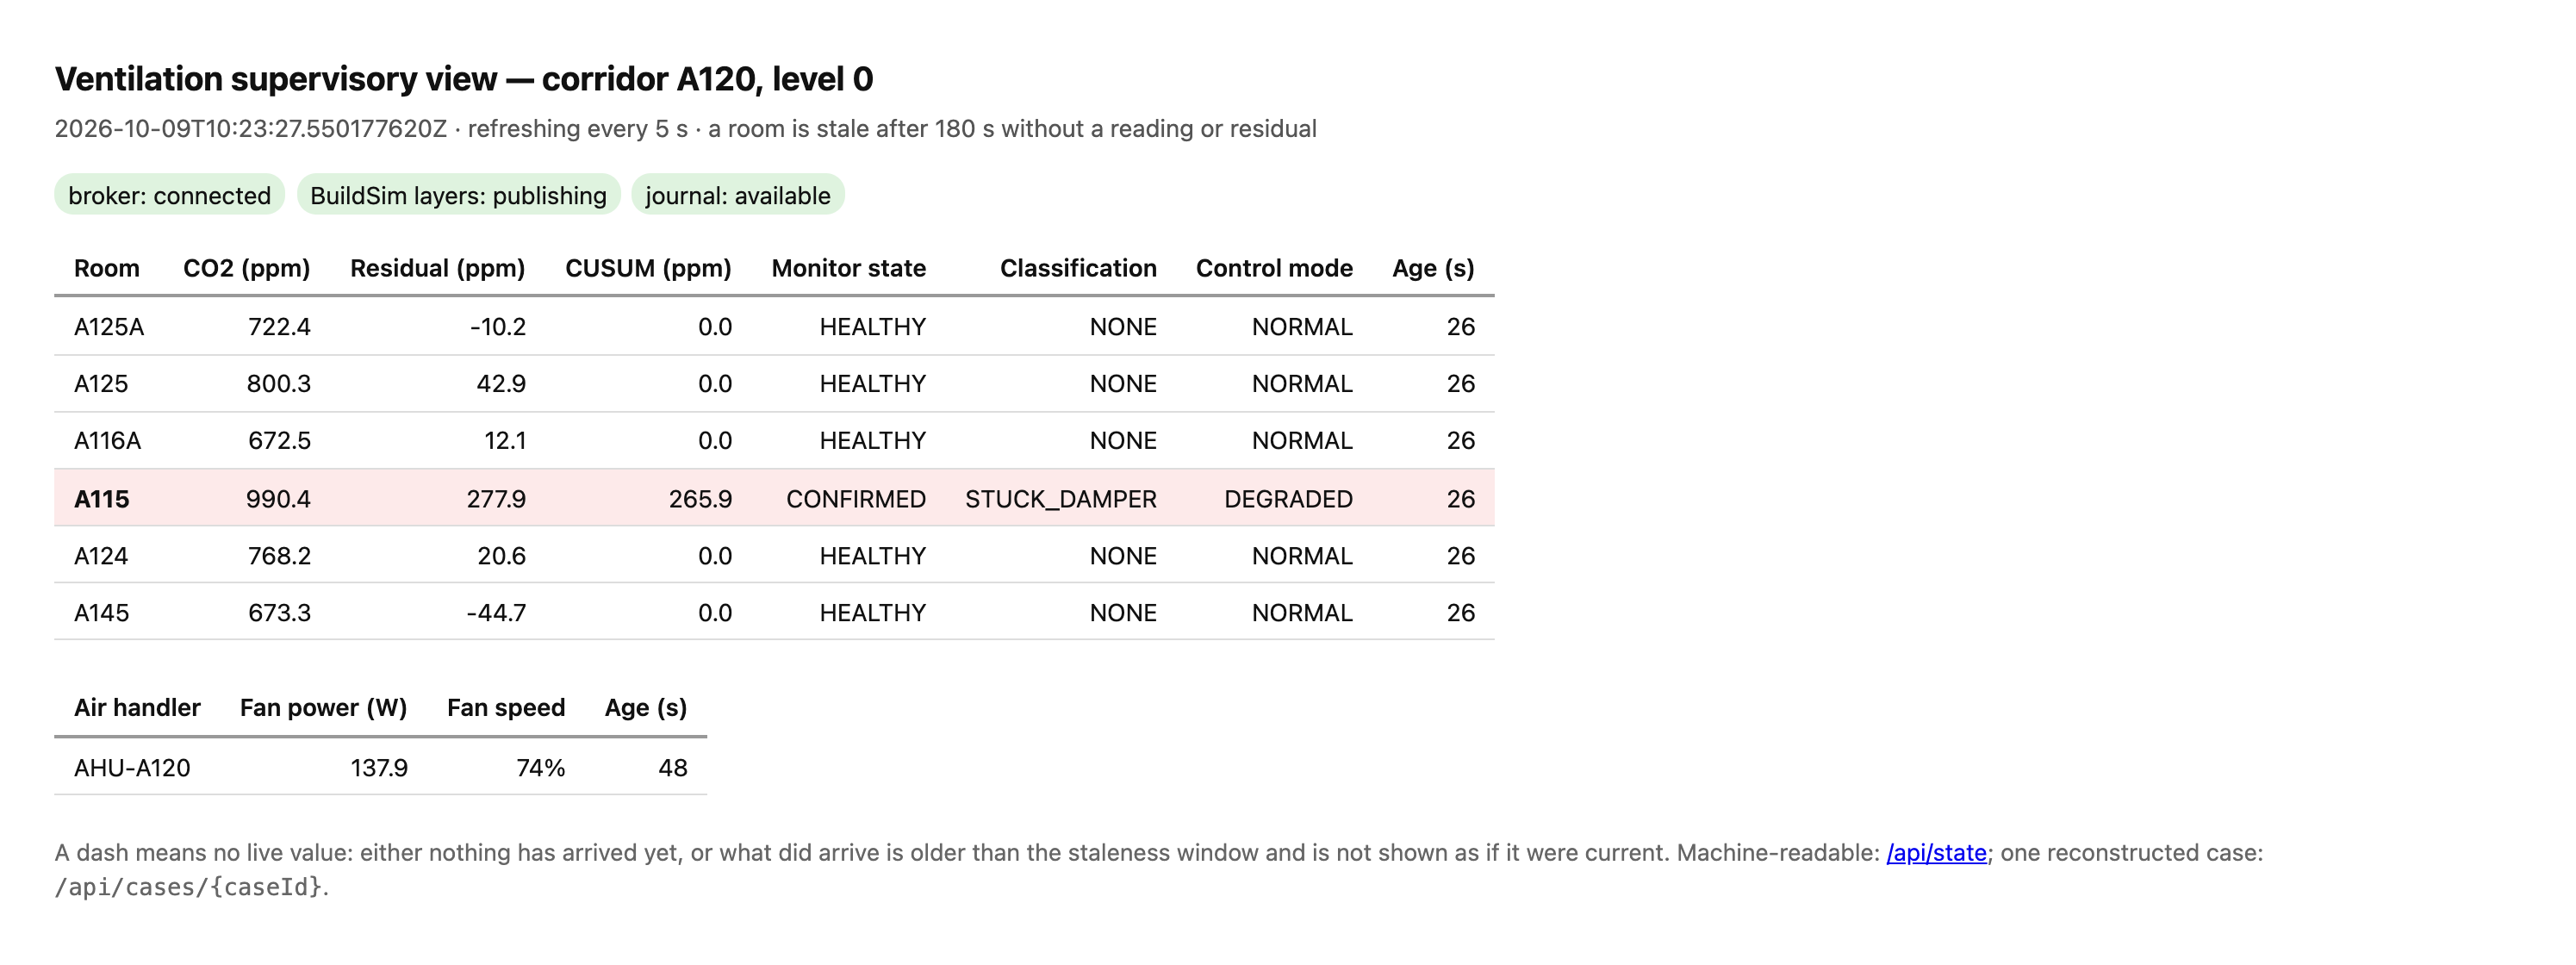
\includegraphics[width=\linewidth]{screenshots/dashboard-confirmed.png}
\caption{Simulated 10:23:27, the same run. A115's row is pink and bold: 990.4~ppm, residual
277.9~ppm, CUSUM 265.9~ppm, \texttt{CONFIRMED} / \texttt{STUCK\_DAMPER} / \texttt{DEGRADED}, with
the air handler at 137.9~W and 74~\%. The other five rooms are \texttt{HEALTHY} at CUSUM 0.0,
which is R-7's isolation visible in one frame. All three dependency pills are green, including
\texttt{BuildSim layers: publishing}.}
\end{figure}

\begin{figure}[!htbp]
\centering
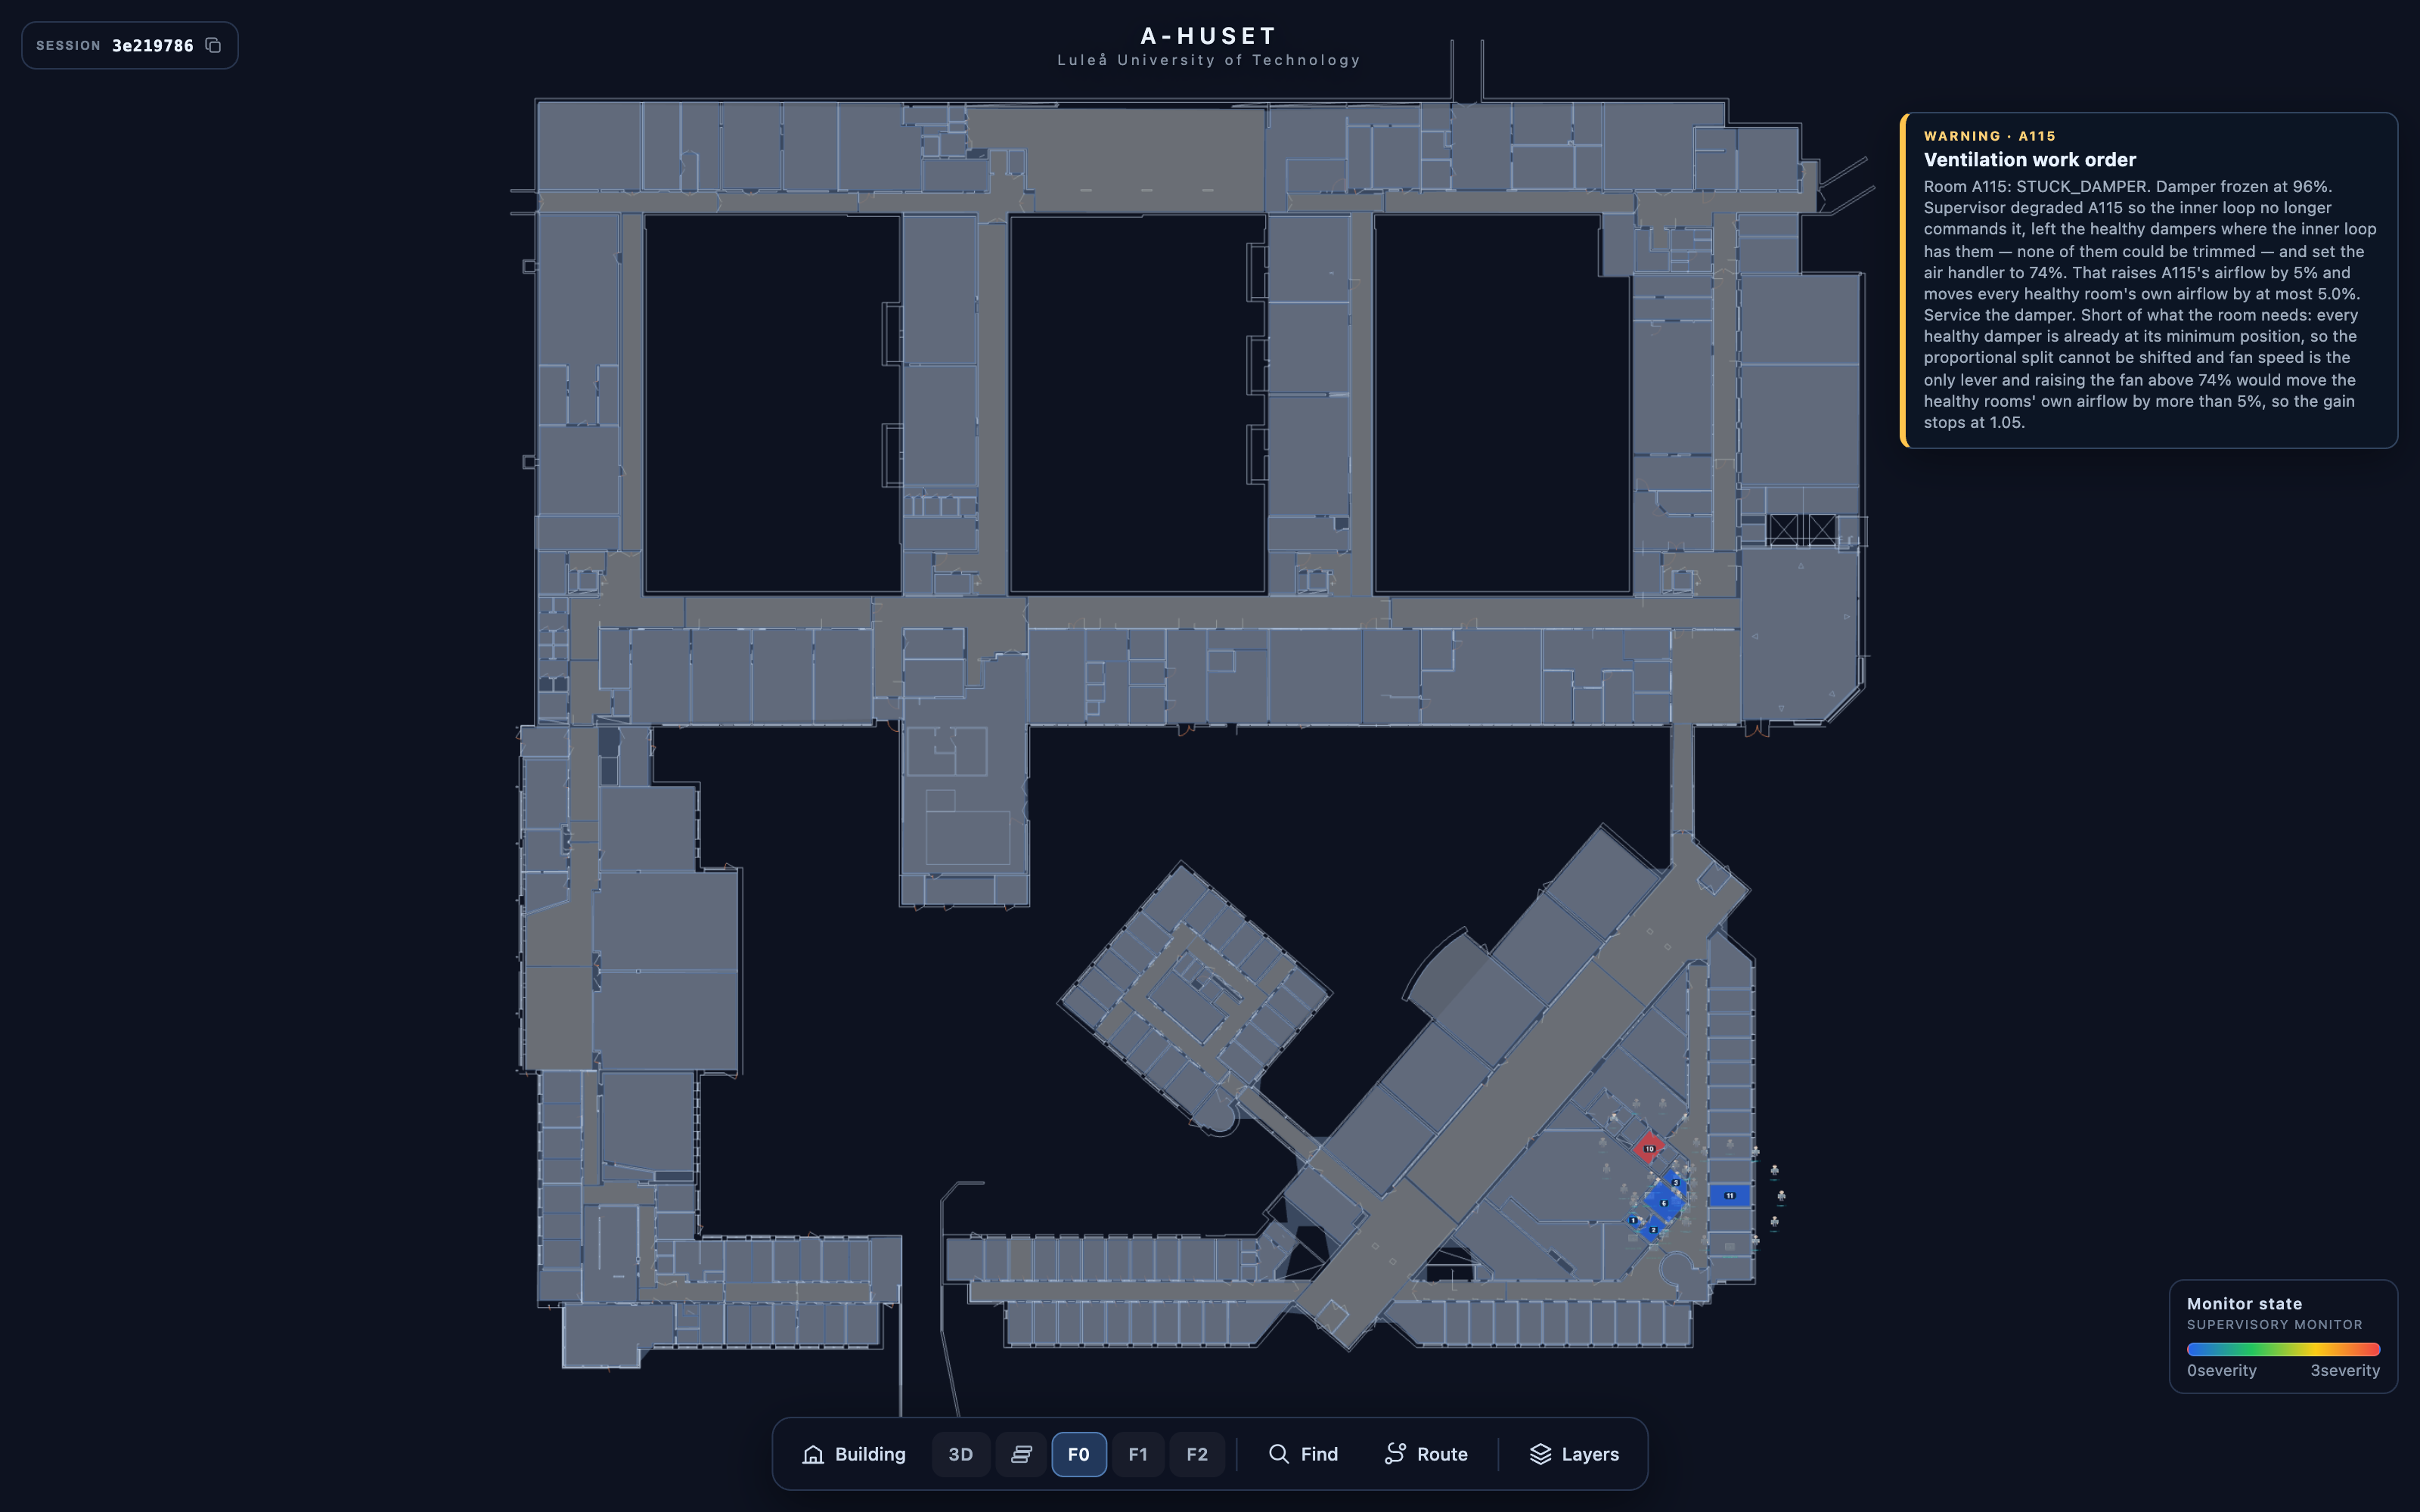
\includegraphics[width=\linewidth]{screenshots/buildsim-state-workorder.png}
\caption{The same instant on BuildSim's own floor plan, \texttt{?layer=state}. A115 is the single
hot room. The panel on the right is rendered by BuildSim from the alert the \emph{supervisor} PUT,
and it names the diagnosis, the action taken and the bound the plan ran into: the fan cannot be
raised above 74~\% without moving the healthy rooms' own airflow by more than 5~\%, so the gain
stops at 1.05. The legend at the lower right is the severity scale the \texttt{state} layer is
painted on.}
\end{figure}

\begin{figure}[htbp]
\centering
\begin{minipage}{0.48\linewidth}\centering
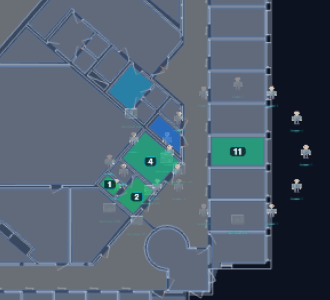
\includegraphics[width=\linewidth]{screenshots/buildsim-layer-co2.png}\\[2pt]
{\footnotesize\texttt{co2}: A115 at 562~ppm, second \emph{lowest} of the six}
\end{minipage}\hfill
\begin{minipage}{0.48\linewidth}\centering
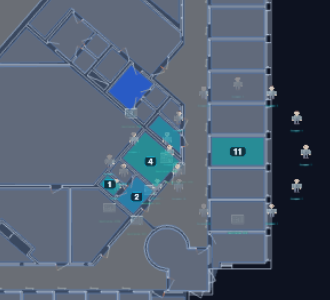
\includegraphics[width=\linewidth]{screenshots/buildsim-layer-residual.png}\\[2pt]
{\footnotesize\texttt{residual}: A115 at the scale floor, $-100$}
\end{minipage}

\vspace{6pt}
\begin{minipage}{0.48\linewidth}\centering
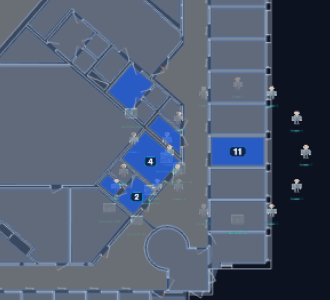
\includegraphics[width=\linewidth]{screenshots/buildsim-layer-cusum.png}\\[2pt]
{\footnotesize\texttt{cusum}: A115 at 0.0, like every other room}
\end{minipage}\hfill
\begin{minipage}{0.48\linewidth}\centering
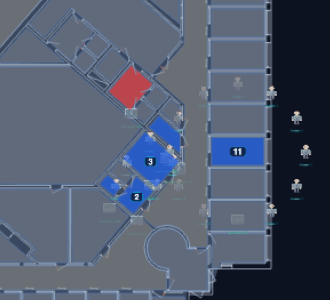
\includegraphics[width=\linewidth]{screenshots/buildsim-layer-state.png}\\[2pt]
{\footnotesize\texttt{state}: A115 at severity 3, the only non-zero room}
\end{minipage}
\caption{Corridor A120 painted by all four layers at one instant, simulated 11:40:55, with A115
latched and \texttt{COMPENSATING}. \textbf{This is the argument of Section \ref{sec:12}, measured rather than
asserted.} Compensation has done its job, so on \texttt{co2} the broken room is the second coolest
on the floor (562~ppm against its neighbours' 478--747), on \texttt{residual} it sits at the bottom
of the scale, and on \texttt{cusum} it is indistinguishable from five healthy rooms. Only
\texttt{state} still says the equipment is broken. \textbf{This figure could not be taken before
the room-layer defect below was fixed}, because three of these four layers never reached BuildSim.}
\end{figure}

% The four-layer frame is most of a page on its own, so it cannot follow the other two. This flushes
% it before H.2 begins rather than letting it land in the middle of H.2's prose.
\clearpage
\subsection{Two defects the capture found, and one limit it exposed}\label{sec:H.2}

\textbf{The layers were overwriting each other.} \texttt{/api/room-layers} is a collection
endpoint and a PUT replaces the whole collection, exactly as \texttt{/api/alerts} does, and the
dashboard was publishing its four layers one at a time, so each call erased the one before it.
Only the last layer of the enum, \texttt{state}, ever reached BuildSim; the other three selected
nothing. Every individual PUT returned 200, so nothing anywhere said so, and the adapter's own
work-order path had the collection semantics right the whole time two methods away. The fix is to
send every layer on every call, and the regression test drives a real HTTP stub rather than a mock,
because the defect was in what went over the wire. A mock of the adapter's own method would have
asserted the bug. The run above confirms it against the real stack and not only the stub:
\texttt{GET /api/room-layers} returns \textbf{four layers of six zones each}.

\textbf{A compensated room is painted exactly like a dead sensor.} At the instant of the four-layer
figure A115's true residual was $-303.9$~ppm. The \texttt{residual} layer's range starts at $-100$,
so \texttt{RoomLayer.onScale} clamps it to $-100$, and $-100$ is also the value that same method
returns for a \emph{stale} room, because the bottom of the scale is the only no-data encoding
BuildSim's layer API offers. On that layer a deeply compensated room and a room whose sensor has
died are therefore the same colour. The range itself is not the error: it was set from measured
healthy residuals spanning $-76.5$ to $+80.3$~ppm and a stuck damper's post-command mean of
507.8~ppm, and widening it to reach $-400$ would spend most of the scale on a regime the operator
almost never reads, making ordinary healthy variation invisible. So this is recorded as a limit
rather than patched: the dashboard table carries the true number one click away, and the
\texttt{state} layer already carries the fact that matters. It is also a limit that \emph{only
became observable} once the layers started arriving at all.

\textbf{\texttt{SUSPECT} cannot be photographed, and now that is measured.} A 1~Hz poll of
\texttt{/api/state} across the whole run caught A115 in \texttt{SUSPECT} in \textbf{2 of 295
usable samples} (296 polls were written and the last was truncated by the teardown), CUSUM 108.5 then 153.5~ppm, on residuals of 274.9 and 190.8~ppm, against a page
that refreshes every 5~s. A state that persists for two seconds may never be drawn at all, so it
is evidenced from the \texttt{decisions} journal and from the poller, and the screenshots are taken
only at states that latch. The instrument, not the intention, is what decides which evidence a
behaviour can carry.

\section{Risks and critical reflection, in full}\label{sec:I}

\S\ref{sec:13} states each finding, its verdict and its bound. This appendix carries the mechanism behind
each one. The subsection numbering follows \S\ref{sec:13} so a reader can move between them.

\subsection{Four functional holes, two of which are now closed (\texorpdfstring{\S\ref{sec:13.1}}{13.1} in full)}\label{sec:I.1}

\textbf{A damper stuck \emph{wide open} is invisible at the deployed setting.} The statistic is
two-sided: the lower arm is the exact mirror of the upper one, $S_\text{low} = \max(0, S_\text{low}
- r - k)$, sharing $k$ and $h$ so that symmetry cost no new tuning parameter. The deployed default
is the \emph{guarded} lower arm, driven by the measurement against the trajectory of an empty room
clamped at the 420 ppm outdoor concentration, and it is what Section \ref{sec:11.2}'s headline figures are
measured on. Two experiments deliberately run the arm \emph{off} beside it, as a control rather
than as a configuration: 180 of T-34b's 540 observed rooms and one of T-26's four regimes. That guard is
what catches the low-side fault with a safety consequence: a sensor drifting downward makes the
inner loop believe the room is cleaner than it is and \emph{under-ventilate an occupied room}, and
it betrays itself by reading below the outdoor concentration, which no amount of ventilation can
produce. What the guard cannot catch is the other low-side fault. ``Everybody left the room''
explains a room that stopped getting stuffier at least as well as ``the damper ignored the close
command'' does, and nothing inside a ten-minute judging window separates them, so a damper stuck
wide open stays \texttt{HEALTHY}. The unguarded setting sees both and costs more false confirmations
than R-3 allows, which the monitor's own fault-free-week test measures. That is the honest form of
this hole: an observer with no occupancy signal \emph{cannot} have both, and the choice was made in
R-3's favour.

\textbf{\texttt{serviced()} had no transport, so a latched false positive could not be cleared in
deployment. And now it has one.} \texttt{FaultCase.serviced()} is the only exit from a latched
case, and for most of this project's life nothing reached it: no MQTT topic, no REST endpoint, no
dashboard action, only the unit tests and the harness. A false latch was \textbf{permanent} and the
technician who repaired the damper had no way to tell the system so. That hole is closed.
\texttt{ServiceReported} travels on \texttt{service/\{zone\}}, \texttt{fault-monitor} subscribes to
it through an adapter that validates the report against the open case, and the dashboard exposes
\texttt{POST /api/zones/\allowbreak \{zone\}/cases/\allowbreak \{caseId\}/serviced}, answering 202 when it is accepted, 404
for a room or case that does not exist, 409 when that case is not latched, and 503 when the broker
is unreachable. The whole
\texttt{CONFIRMED}~→~\texttt{COMPENSATING}~→~\texttt{SERVICED}~→~\texttt{WARMUP}~→~\texttt{HEALTHY}
lifecycle is executable and tested end to end, including that a reported repair unwinds the
compensation and hands the five healthy rooms back to the inner loop. \textbf{This matters most to
the latching trade-off below}, whose whole argument is that a false positive costs only one
technician visit: an argument that was being made against a system in which it cost that visit
\emph{and} a permanently wrong work order. It is now true as stated. One thing is deliberately
absent: there is no button on the HTML status page, because that page is server-rendered with a
meta refresh and no JavaScript, so a form post would land the operator on a JSON body. The endpoint
is the operator path.

\textbf{Blocked filters are plant-wide by construction, so the classifier's hardest discrimination
is never tested.} The statement ``the three signatures may collapse into two'' is too soft. In
\emph{this} simulator they cannot collapse: a blocked filter is plant-wide by construction, so it
starves all six rooms and a stuck damper never does, and the common-mode count separates them
trivially. The ambiguity that would really arise in a building (a partial obstruction in one duct
branch, which reads as both a partly stuck damper and a partly blocked filter) \textbf{is not in
the fault model at all}. The enumeration cannot express it. So a clean confusion matrix from the
classifier would be weak evidence rather than strong, and reporting one without this paragraph
would be misleading. The risk register forbade inventing a fourth \emph{signal} to rescue a
three-way taxonomy; it never forbade a fourth \emph{fault}, and adding the ambiguous one is what
would have made the classifier's evaluation worth reading.

\textbf{And worse than untested: the \texttt{BLOCKED\_FILTER} branch of the classifier is
unreachable with this physics.} This is the finding I least expected and the one I would lead with
in the oral. A unit test pins it deliberately: it injects a blocked filter and asserts the
classification is \texttt{UNCLASSIFIED}, with a message saying that if it ever starts classifying,
the test's finding is out of date. Two structural reasons, and neither is a bug to be patched:

\begin{itemize}
\tightlist
\item \textbf{The split only redistributes a fixed total.} $Q_i = Q_\text{fan}\,a_i/\sum a_j$ means
  no damper command can move all six residuals the same way; a blockage shrinks $Q_\text{fan}$, but
  the observer judges \emph{step responses to commands}, and no command it watches produces the
  plant-wide common mode the first branch of the tree requires.
\item \textbf{The generation estimate absorbs the blockage exactly.} From Section \ref{sec:7.2},
  $G_\text{est} = Q\,(C_\text{measured} - C_\text{out})$ is learned from quasi-steady state. With a
  blockage, the true flow is low by $(1-\beta)$ and the believed flow used in the prediction is high
  by the same factor, so $G_\text{est}$ comes out high by precisely $1/(1-\beta)$, and the two
  errors cancel in the predicted steady state. Only the \emph{time constant} differs, and the
  residual the CUSUM sees never develops the bias it needs. The observer's defence against not
  knowing occupancy is, in other words, also a defence against noticing a blocked filter.
\end{itemize}

What saves the outcome from being useless is that the classifier reports its evidence even when it
declines to name a cause, so the work order still states the measured plant power excess and that the
residual is not common mode: a technician is sent to the air handler with the right number, by a
system that admits it cannot prove which fault it is. That is the correct behaviour for an
unclassifiable case and it is not the same thing as a working three-way classifier. \textbf{The
honest headline is that of the mechanisms this project set out to name, exactly one is classified:
\texttt{STUCK\_DAMPER}.} \texttt{BLOCKED\_FILTER} can be pointed at but never confirmed, for the
structural reason above. And \texttt{SENSOR\_DRIFT}, which this paragraph used to call classified
``once a night of overnight-floor history exists'', is \textbf{never emitted at all}, in 0 of 76
runs from a drift ramp and 0 of 76 from a step offset (§\ref{sec:7.3}, §\ref{sec:11.5}). Its leaf wants an informative
overnight floor and a matched step response in the same instant, and the two injectable sensor
mechanisms supply one each and never both, because the classification is computed at the confirmation
while one of its inputs needs a day of the fault.

\subsection{The air handler's rating was corrected on measurement (\texorpdfstring{\S\ref{sec:13.3}}{13.3} in full)}\label{sec:I.2}

Run that plant at the normal 0.7 and it delivers 294 l/s against a 411.4 l/s design total, 71 \% of
design flow, and the consequence was not subtle: with \textbf{nothing broken} no room could be held
below 1000 ppm at design occupancy and the monitor confirmed a fault in all six, because a uniformly
starved building looks exactly like a faulty one. Sizing instead from $\Sigma$ design $\div\ 0.7$
separates the two jobs the rating was doing at once: the plant covers its design condition at the
speed it actually runs, and the margin to $s=1$ is reserved for compensation. The fix is not free,
and this is the honest cost: \textbf{margin masks faults}. At the corrected rating a filter blocking
35 \% no longer starves the rooms enough for the monitor to confirm it, where at the undersized
rating it did. Detection sensitivity was being bought with occupant comfort, which is the wrong
currency, so the trade is made deliberately in comfort's favour and its cost is stated here rather
than hidden. The correction is now measured rather than argued: at the corrected rating the
no-fault arm of T-26 holds every occupied minute at or below 1000 ppm at design occupancy, on all
five seeds, in every regime (§\ref{sec:11.2}). That is the figure the earlier sizing scored 0.000 on.


\subsection{The CUSUM margin, and why $h$ was never the knob (\texorpdfstring{\S\ref{sec:13.4}}{13.4} in full)}\label{sec:I.3}


The worst healthy seed peaked at 149.1 ppm against $h$ = 150 ppm at $\sigma$ = 30 ppm, over three
hours in one room: a \textbf{0.9 ppm margin}, with the next seed at 91.6 ppm, so it is a tail draw
and not a design property. R-3 asks for at most one false alarm per simulated week \emph{across six
rooms}: the same statistic over far more samples, six times over. The mitigation is persistence
rather than a higher limit: requiring the statistic to hold above $h$ for two consecutive cycles
removes a tail draw, which the next sample erases, while a stuck damper clears $h$ every cycle.
Raising $h$ instead trades R-3 against R-1, and the sweep in §\ref{sec:11.1} prices that trade: 8σ costs about
a minute of delay, and 4σ already gave one false alarm in twenty short runs. Siegmund's
ARL$_0 \approx 1.1\times10^{5}$ samples $\approx$ 79 days is analytic, on i.i.d. noise which the
production residual is not. And the measurement contradicts it. Over 20 fault-free simulated weeks
of all six rooms the monitor raises \textbf{0.55 confirmed cases per week against R-3's limit of
one}, with \textbf{16 of 20 weeks clean} and a worst week of 6, against 1.30 per week and 9 clean
weeks before ADR-0010, while on the same tuning R-1's stepped p95 is 6 min against a 15 min budget
(§\ref{sec:11.2}). So the trade this section prices came out on R-3's side of the line, but it was not the
binding trade, and that is the correction this section needs. \textbf{$h$ was never the knob.}
ADR-0010 attributed the failure, and the defect was in the \emph{reference} the limit is applied to
rather than in the limit: both plausibility guards were being corrected 30 \% of the way onto every
reading, so each CUSUM arm was accumulating a filter error instead of a residual, which is what put
the statistic into the very i.i.d. regime the analytic run length assumes and is why the analytic
figure was contradicted so badly. Correcting the lower arm's half of it halved the rate with
$k$ = 30 ppm and $h$ = 150 ppm \emph{untouched}. The response taken is therefore unchanged and
better supported than when it was taken: $k$ and $h$ stay where the spike put them rather than
being retuned until R-3 passes, because retuning a limit on the experiment that failed it is the
same methodological error §\ref{sec:13.10} already names, and the measurement now says the limit was not the
defect. What R-3 still fails on is the worst week, which is seed 2 at six confirmations, all on the
upper arm; the upper arm's half of the same defect is measured, meets R-3 outright, and was
declined because it costs three other requirements (§\ref{sec:11.2}, ADR-0010).

\subsection{R-7 at design occupancy, and the two bounds on that finding (\texorpdfstring{\S\ref{sec:13.5}}{13.5} in full)}\label{sec:I.4}

Until this revision R-7 was reported as met, full stop, on 270 observed rooms. It was met on the
occupancy regime it had been run in. Running the same experiment with every room at its design head
count fails \textbf{231 of 270}, and the shape of the failure is the result.

The two failing clauses are \textbf{disjoint}: 215 observed rooms were themselves \emph{accused of a
fault they did not have}, and 16 more sat outside the 5 \% airflow band at a worst deviation of
0.058919: 215 plus 16 is the 231. They attribute in opposite directions, and the supervisor-dead
pass is what separates them. The accusations run 85 of 90 rooms with the supervisor \emph{dead}
against 130 of 180 with it live, so they belong to the regime and the monitor rather than to the
response to the fault: compensation slightly \emph{suppresses} them. The airflow breaches run 0 of
90 dead against 16 of 180 live, so that half is the compensation's own cost and nothing else's.

\textbf{So the larger half of R-7's design-occupancy failure is R-3's false-alarm rate, measured by a
different experiment, in a regime R-3's own replay never visits.} That is the second time this report
has had to say it: §\ref{sec:11.2} records the same pattern inside R-2, where two of five design-occupancy
seeds fail because every room is latched by false alarms and the trim lever is gone. \textbf{R-3 is
not one failing requirement among four; it is the one whose failure the other three inherit}, and
stating it that way is worth more than three independently reported shortfalls. ADR-0009 predicted
exactly this collision and noted that no experiment asserted R-7 in that regime. One does now.

Two bounds on the finding. The first is that \texttt{CompensationPlan.worstHealthyFlowDeviation()}
\textbf{cannot falsify this requirement} and should stop being quoted beside the figure that can: it
reaches 0.0500 and no further in any regime, because the solver caps the fan at the speed that makes
the figure exactly the tolerance and then reports that cap. The second is that the 5 \% bound's
\emph{reference plant} is ambiguous: the solver bounds its claim over each latched room's
latch-time opening, the independent recomputation over its pre-latch one, and the two coincide until
a second room latches inside one episode, which the drawn weekday never does and design occupancy
routinely does. Both are defensible readings of ``before the compensation'' and ADR-0008 never says
which. That is an ADR-level question, not a code change.

\subsection{The third diagnostic signal is blind after a confirmation (\texorpdfstring{\S\ref{sec:13.6}}{13.6} in full)}\label{sec:I.5}


§\ref{sec:7.3} records that the stuck-damper leaf fires on two signals rather than three, because a probe can
only be requested once a case is latched and no step has been judged at classification time. The
obvious repair is to reorder: latch as usual, withhold the diagnosis, ask for the probe immediately,
and name the fault when the step lands. \textbf{It was built, measured over 176 paired runs on
identical seeds, and not kept.} Detection moves in 0 of 88 pairs and the fault is named on a
genuinely judged step in 28 of the 39 runs that defer, against none before. And the settled
classification is identical in all 88 pairs, because the judged step reads \texttt{MISSING} for a
stuck damper, a blocked filter, nine rooms whose dampers are in perfect health, and the run with
nothing injected.

The cause is a located defect older than the ordering, and it is the useful part.
\texttt{ZoneObserver.\allowbreak recordStepAmplitude} measures the amplitude's \emph{measured} leg against
\texttt{predictedAtStep} while the predicted leg is also against \texttt{predictedAtStep}, so the
measured leg carries the standing residual as a constant offset. And the anchor-gain pull that
would make that baseline legitimate is switched off while a case is open, so at the confirmation the
prediction is stale by exactly the residual that confirmed it. \texttt{ZoneObserver.measuredAtStep}
is assigned for this purpose and never read. On a 600 ppm offset with a healthy damper that answers
its probe by dropping 300 ppm, the amplitude ratio runs from $-7.0$ to $-0.8$.

\textbf{And correcting that baseline makes the reorder worse, not better}, which is the finding worth
defending. Measured as an unlanded counterfactual, the corrected signal takes T-15's diagonal from
18/44 to 15/44: it reads \texttt{MATCHED} on 3 of 8 genuinely stuck dampers and \texttt{MISSING} on 5
of 11 healthy ones, because by the time a probe can be commanded the supervisor has degraded the
zone, raised the fan and trimmed the other five, so the room's answer is mostly the compensation's. The 18/44 baseline reproduces on the current code; the 15/44 was measured on a one-line patch that was then reverted, so it is the one figure in this report that cannot be re-derived from the repository as it stands.
This is the masking the latching argument in §\ref{sec:13.8} already rests on, arriving one level down, in the
diagnosis rather than in the clearing policy. \textbf{A three-signal stuck-damper diagnosis therefore
needs a step judged \emph{before} a case opens} (the inner loop's own trims, read against a
baseline that survives them) rather than a probe requested after the response to the fault has
begun. That is design work, and it is the one concrete thing this report would hand to a successor.

\subsection{Scope, and the debts taken knowingly (\texorpdfstring{\S\ref{sec:13.9}}{13.9} in full)}\label{sec:I.6}

\textbf{Legitimate scope.} Six rooms on one floor behind one air handler is not a building, but the
shared fan makes R-7 non-trivial: keeping five rooms unchanged while compensating the sixth is
something the supervisor must actively do. Simulated time through \texttt{ClockPort} is legitimate
too, but the reproducibility it buys has to be stated precisely, because the obvious phrasing is
false of half the system. \textbf{In the offline harness the replay is reproducible bit for bit}:
the clock is a \texttt{SimulatedClock}, the bus is a list and the iteration order is fixed, so the
draws are identical run to run, which is exactly what R-3's false-alarm count needs.
\textbf{In the containerised demo profile it is not}, and that is measured rather than suspected:
four runs on identical \texttt{SEED}, \texttt{TIME\_SCALE} and \texttt{START\_AT} confirmed A115 at
simulated 10:16, 10:17, 10:19 and 10:23, a spread of seven simulated minutes. The cause is that
the sensor model draws once per Euler sub-step and the sub-step count follows \emph{real} elapsed
time, so host scheduling decides how many draws a simulated minute contains. The offline number is
the one every requirement is argued from; the demo profile is for showing the system work, not for
measuring it. What simulated time does \emph{not} exercise either way is anything that
appears only over real duration: scheduler jitter, clock drift, broker backpressure, memory growth.
R-6's cycle time is the only result in the plan that touches timing at all.

\textbf{Debts.} Skipping a DTO layer is justified by lock-step single-author deployment, but it makes
a domain refactor a wire-format break and is wrong the moment any consumer deploys independently.
Having no message replay is similarly contingent: R-3's evidence comes from a seeded harness rather
than from the broker, so the evaluation never needs replay, but in a real deployment a monitor
restart loses the residual history it was accumulating, and R-5 then rests entirely on the journal.
Three smaller debts, all three of which have since been \textbf{corrected} and are kept here because
what they were is worth more than that they are gone. The first: \texttt{Topology} could express a
synthetic zone set larger than six but nothing in any container wired it, so the capability existed
and R-6 could not be run from the deployed system. \texttt{ZONE\_COUNT} is now an environment
variable all \factAuthoredServices{} project-authored containers read, and the stack was brought up and watched at 12
and at 58 zones, 58 being a hard ceiling that belongs to BuildSim rather than to the monitor,
since it refuses to host equipment in a room its floorplan does not have. \textbf{R-6's breaking
point therefore remains a harness measurement}, and the two ceilings are three orders of magnitude
apart. The second: ADR-0005 and ADR-0006 argued in the superseded access-control vocabulary (doors,
badges, requirement IDs that no longer exist) against requirements the project had replaced. Both
were retargeted, and then checked line by line against the source tree, which found that the
retargeted prose made three further wrong statements about the code: an interface inventory listing
five where the tree has fifteen, a claim that five components carry the full
\texttt{boundary}/\texttt{control}/\texttt{entity} structure, and device-process line counts given as
``around a hundred each'' against 297 and 237. \textbf{Correcting a document can introduce fresh
errors of its own}, and only a pass against the tree finds them. The third, that the monitor's
parameter record documented its plausibility ceiling as 1.0 while the code used 1.25, sat in the one
parameter that decides how desensitised the detector is, which is the worst place to have two
different numbers written down: \texttt{MonitorParameters} now reads 1.25 in both its javadoc and its
defaults, and the same pass removed two further false claims from that record (ADR-0010).

\textbf{A fourth of the same shape was found and closed in this pass, and it was the most expensive
of them.} The probe step had \emph{two} numbers (\texttt{MonitorParameters.probeStepIncrease} at
0.20 and \texttt{SupervisionService.PROBE\_STEP} at 0.25), and the consequence was worse than
duplication, because the monitor \emph{asks} in the evidence an operator reads while the supervisor
\emph{acts}. The system published ``step to 0.35'' on \texttt{faults/\{zone\}}, journalled that, and
commanded 0.40: \textbf{it was telling the operator one thing and the building another}. There is one
owner now, in \texttt{shared}, because the amplitude has to mean the same thing to the component that
requests it and the one that commands it. Why the divergence survived is worth keeping: the request
is prose inside \texttt{FaultStateChanged.evidence}, a \texttt{List<String>}, so the supervisor could
not read the amplitude off the wire without a schema change four components decode. The change was
taken on the operator-facing argument and \textbf{not} on a measurement (no requirement verdict
moved), and it had one measured side effect worth more than the fix: a 0.05 change in one amplitude
moved \textbf{ten of T-34b's design-occupancy rows from pass to FAIL}, by causing one extra room to be
falsely accused on one seed. That is R-3's false-alarm rate again, and it says the design-occupancy
regime is not merely failing but \emph{unstable}.

\textbf{One debt was addressed, and what it cost to try is more interesting than the debt.}
T-15 found that \texttt{ZoneMonitor.stepShapeUnchanged()} collapsed ``no evidence'' into ``evidence
of a missing response'': it returned \texttt{false} when the step-amplitude ratio was \texttt{NaN},
and \texttt{NaN} is what the observer reports when \emph{no step has ever been judged}. The
classifier's stuck-damper leaf read that as the commanded step having produced no matching
response, so \texttt{STUCK\_DAMPER} could be emitted for a room the monitor never asked to move:
9 of 57 drift runs confirm by exactly that route.

The signal is now a three-valued type, so the conflation cannot be written by accident again. The
\emph{strict} fix, requiring positive evidence of an unanswered step, was then tried, and
\textbf{it emptied the leaf}: the one cell on T-15's diagonal went to \texttt{UNCLASSIFIED} and the
tree classified nothing at all. The cause is an ordering problem, not a logic one. A probe is
requested through the evidence on \texttt{FaultStateChanged}, so a case must be open before a step
is commanded, and \textbf{the step-amplitude signal therefore arrives after the decision it exists
to inform}. The \texttt{NaN} was not an incidental bug; it was the only thing making that leaf
reachable, and the taxonomy has been quietly running on two signals rather than three for its whole
life.

What is in the repository is the honest middle: the leaf still fires on localisation and flat fan
power, and every diagnosis reached without a judged step now carries an explicit entry saying it
rests on two signals, that the room has not been asked to move and so has not failed to answer, and
that a probe has been requested to settle it. Behaviour is unchanged (T-15's, T-24's and T-25's
result files reproduce byte for byte, so no number in this report moved), and the weakness is now
in the work order an operator reads instead of inside a boolean. \textbf{The real fix is to command
a probe step before classifying rather than after}, which reorders the diagnosis pipeline and would
trade detection delay for diagnostic confidence. That is a design change with its own experiment
attached, and it is the first thing this system should do next.

\section{Risk register}\label{sec:J}

The register \S\ref{sec:13.11} points at. Each row is a risk or an assumption, its impact, and the response
with its current status.

\begin{longtable}[]{@{}
  >{\raggedright\arraybackslash}p{(\columnwidth - 4\tabcolsep) * \real{0.32}}
  >{\raggedright\arraybackslash}p{(\columnwidth - 4\tabcolsep) * \real{0.26}}
  >{\raggedright\arraybackslash}p{(\columnwidth - 4\tabcolsep) * \real{0.42}}@{}}
\toprule
\textbf{Risk or assumption} & \textbf{Impact} & \textbf{Response, and its status} \\
\midrule
\endhead
R-3 fails at the seven-day six-room horizon & The headline false-alarm claim goes &
\textbf{Measured, and it does fail}: 0.55 confirmed cases per fault-free week against a limit of 1
over 20 weeks, 16 of 20 weeks clean, worst week 6, which is the scored criterion (§\ref{sec:11.2}); 1.30 per
week with 9 clean weeks before ADR-0010 attributed the cause. Persistence of two cycles is in place
and is not enough; the mechanism is now named and half of it is corrected, and the half that would
meet R-3 outright costs R-1's closed-loop arm, T-27 and R-7 \\
A damper stuck wide open is invisible under the guarded lower arm & Five neighbours quietly robbed
of air by the split, and a controller that never learns its damper is dead & The two-sided statistic
\textbf{is implemented} and its guarded arm is the deployed default, which catches the
safety-relevant low-side fault; the unguarded setting catches both and costs more false confirmations
than R-3 allows. \texttt{DAMPER\_STUCK\_OPEN} now \textbf{exists} as a classification and three
things branch on it, so the fault is expressible and actionable, but naming it did not make it
detectable, and the trade is unchanged. Note the correction: a damper frozen open does \emph{not}
waste fan energy, because the shared fan delivers a fixed total at a given speed and the six openings
only divide it. It misallocates \\
\texttt{serviced()} had no transport & A false latch would be permanent in deployment &
\textbf{Implemented}: \texttt{service/\{zone\}}, a validating adapter, and
\texttt{POST /api/zones/\{zone\}/cases/\{caseId\}/serviced}; the full lifecycle is tested end to end \\
The detector shares its generator's assumptions & Detection numbers do not transfer & Stated as a
bound on every detection claim; a second independent fault model would be needed \\
Occupancy-dependent detection delay & A lightly occupied room hides its fault &
\textbf{Measured, and the risk is real}: stratifying the closed-loop runs by the head count at the
ignored command gives 0 of 4 confirmed at 0.625 of design occupancy, then 77 min median at 0.875
and 31 min at 1.00 (§\ref{sec:11.2}). The plausibility ceiling limits false confirmations and \emph{is} the
mechanism of this delay. What is still unmeasured is a sweep that holds the occupancy ratio as a
controlled input over a wider range than a drawn weekday visits \\
The ambiguous fault is absent from the model & A clean confusion matrix would mean little & Add a
per-branch obstruction to the generator; not done \\
\texttt{BLOCKED\_FILTER} is unreachable with this physics & One of the three named faults can be
pointed at but never confirmed & Pinned by a test that asserts \texttt{UNCLASSIFIED} so the finding
cannot rot; the work order still carries the plant power excess \\
R-6's number comes from the harness, not from a container & R-6 is measured for the monitor
rather than for the deployed system & The entity-layer capability is wired to the harness and
measured there (§\ref{sec:11.2}); every container reads it through \texttt{ZONE\_COUNT}, and what stays
harness-only is the breaking point rather than the capability \\
Fan saturation & Compensation degenerates to redistribution, gain 1.296 & Bounded by a 5 \% healthy
tolerance and reported as the achieved gain; working as designed \\
The healthy-damper trim is the only lever, and every damper sits on its floor & Compensation is a
no-op and the supervisory loop is worth nothing, or less than nothing & \textbf{Measured, and it
did happen}: $+0.000$ of occupied minutes on the drawn weekday and 34 ppm \emph{worse} than no
supervisor at design occupancy. Fan speed is now spent once the trim is exhausted (135 ppm of help
in that regime), bounded by the 5 \% healthy tolerance because the lever is not selective, and that
5 \% is itself kept on a sweep rather than assumed (ADR-0009). The 0.05 cases per week once charged
to this lever against R-3 is withdrawn: the allowance does not move R-3 at any setting from 0.05 to
0.99, and ADR-0010 attributes those confirmations to the plausibility guards instead (§\ref{sec:11.2}) \\
Broker is a single point of failure & Readings stop flowing & Restart policy; a dead publisher
produces silence, which drives \texttt{BLIND} rather than a wrong decision \\
\bottomrule
\end{longtable}

\section{The test plan, the test suite and the evaluation harness, in full}\label{sec:K}

\subsection{The test plan, with each test's expected result and its evidence}\label{sec:K.1}

\begin{longtable}[]{@{}
  >{\raggedright\arraybackslash}p{(\columnwidth - 8\tabcolsep) * \real{0.0683}}
  >{\raggedright\arraybackslash}p{(\columnwidth - 8\tabcolsep) * \real{0.3219}}
  >{\raggedright\arraybackslash}p{(\columnwidth - 8\tabcolsep) * \real{0.1366}}
  >{\raggedright\arraybackslash}p{(\columnwidth - 8\tabcolsep) * \real{0.2146}}
  >{\raggedright\arraybackslash}p{(\columnwidth - 8\tabcolsep) * \real{0.2536}}@{}}
\toprule
\textbf{ID} & \textbf{Test or experiment} & \textbf{Requirement} & \textbf{Expected result} &
\textbf{Evidence, and whether it exists} \\
\midrule
\endhead
T-24 & Detection delay swept against the CUSUM limit $h$, ≥ 20 runs per point & R-1 &
Trade-off curve; p95 ≤ 15 min at the chosen $h$ & \textbf{Run}, 200 runs over six arms: stepped
p95 6 min, 20/20; closed-loop p95 257 min, 15/20 (§\ref{sec:11.2}) \\
T-25 & Model-based monitor against a plain residual threshold, identical seeds, 7-day fault-free
replay & R-1, R-3 & Fewer false alarms at equal delay; ≤ 1 alarm per week & \textbf{Run}: at equal
alarm volume the monitor detects 0.75 against the threshold's 0.15, at a median delay of 74 min
against 312; R-3 fails at \textbf{0.55} confirmed cases per fault-free week, down from 1.30 before
ADR-0010, with 16 of 20 weeks clean and a worst week of 6 (§\ref{sec:11.2}) \\
T-15 & Confusion matrix over the four injected faults on a fixed seed, plus a no-fault arm &
R-1, R-3 & Each fault classified as itself; the no-fault arm silent & \textbf{Run}, 218 runs:
\texttt{STUCK\_DAMPER} named correctly, \texttt{BLOCKED\_FILTER} → \texttt{UNCLASSIFIED} 11/11,
\texttt{SENSOR\_DRIFT} \textbf{never emitted} (0 of 76 from a drift ramp and 0 of 76 from a step
offset), \textbf{one of four mechanisms classified} (§\ref{sec:7.3}) \\
T-26 & Comfort during a latched fault, with and without compensation & R-2 & CO₂ ≤ 1000 ppm for
≥ 95 \% of occupied minutes with compensation & \textbf{Run}: 5 of 5 seeds on the drawn weekday, 0
of 5 at design occupancy, no-fault reference 5 of 5 throughout (§\ref{sec:11.2}) \\
T-27 & Kill each container in turn & R-4 & \texttt{BLIND} with zero fault events; recovery within
one cycle & \textbf{Run} in-JVM, 23 of 23 assertions: \texttt{BLIND} in 4 cycles, 0 fault events,
0 commands on stale data, \texttt{HEALTHY} 3 cycles after recovery (§\ref{sec:11.2}); container kills
\textbf{now also run} against \texttt{docker compose}: five of six rooms \texttt{BLIND} in 12 s,
no diagnosis and no healthy-room command while blind, three-cycle recovery, fan held at 158.3~W
with the supervisor dead; and the restart policy fires on an in-container \texttt{SIGTERM}:
restart count 1, running again within 3 s (§\ref{sec:11.6}). \textbf{The one-cycle recovery
expectation is missed.} It was written before the state machine was, and recovery is routed back
through \texttt{WARMUP} by design, so three cycles is the floor and the harness asserts
$\le$ 5 cycles. R-4's acceptance criterion says nothing about recovery timing, so
its verdict is unaffected; the expectation stated here is what was wrong \\
T-20 & Rebuild a random diagnosis from the journal & R-5 & Inputs, command, residual series,
classification and timestamp all recovered & \textbf{Demonstrated live} in the recorded demo run:
one \texttt{caseId} rebuilt against a real TimescaleDB: HTTP 200, 77\,248 bytes, \textbf{445 events}
(\texttt{evaluation/\allowbreak results/\allowbreak T-23-demo-run.txt}, §\ref{sec:3} status, §\ref{sec:11.6}). The id
was the one that run produced rather than a drawn one.
\textbf{And now tested}: eight integration tests execute \texttt{replayCase}'s real SQL against a
real PostgreSQL, including the one-hour evidence lookback pinned at $-$59, $-$60 and $-$61 min \\
T-28 & Scale zones per monitor to the breaking point & R-6 & The zone count where p95 cycle
exceeds 60 s, and the saturated component named & \textbf{Run}: 25\,600 zones at a p95 of about
6 s measured, $\approx$ 86\,000 extrapolated, \texttt{AhuFlowModel.\allowbreak believedFlowTo} named
(§\ref{sec:11.2}) \\
T-34b & Room isolation: one injected fault per run, rotating the injected room over ≥ 3 rooms &
R-7 & Zero events and no mode change in the other five; their CO₂ and airflow inside the healthy
band & \textbf{Run}, both occupancy regimes, 540 observed rooms: all six rotated, 3 seeds, 3
configurations. Drawn weekday \textbf{0 of 270 failed}; design occupancy \textbf{231 of 270
failed} (§\ref{sec:11.2}) \\
T-29 & Optional learned one-class contender against the CUSUM on identical seeds & R-1, R-3 &
Kept only if it wins & \textbf{Run}, 20 seeds and 30 operating points against a held-out
fault-free week: \textbf{dropped}. To match the monitor's 0.75 detection it costs about 20× the
false alarms (11.25 against 0.55 per week) and 7× the delay (518 against 74 min) (§\ref{sec:11.2}) \\
T-35 & Classify after a probe has been judged, or at confirmation? 176 paired runs on identical
seeds & R-1 & Kept only if it buys classification accuracy at an acceptable delay &
\textbf{Run}: \textbf{not adopted}. Detection moves in 0 of 88 pairs and the fault is named on a
judged step in 28 of the 39 runs that defer against 0 before, and the settled classification is
identical in all 88 pairs, because the judged step reads \texttt{MISSING} for every condition
including rooms whose dampers are healthy (§\ref{sec:7.3}, §\ref{sec:11.2}) \\
T-36 & One observation published on the real broker, consumed by the running
\texttt{fault-monitor} and asserted in the real journal & R-5 & The published observation reaches
the journal through a process this test does not run, unchanged & \textbf{Run}, 2 tests against the
deployed stack: the row carries the published wattage, the publisher's instant rather than the
subscriber's, and \texttt{source = fault-\allowbreak monitor}; and a reading for a room outside
\texttt{ZONE\_\allowbreak COUNT} is journalled nowhere. It injects under an invented \emph{AHU} id,
which touches no room's model. Without the stack both \textbf{skip} with the reason attached \\
T-37 & A latched diagnosis survives a \texttt{SIGKILL} and restart of its container & --- &
What the process concluded outlives the process, so a restart is not a back door through the one
exit the design reserves for a technician & \textbf{Run live on the demo profile}, not in the
suite: \texttt{evaluation/\allowbreak results/\allowbreak T-37-\allowbreak restart-\allowbreak recovery.txt}. The case id
\texttt{779b28fb} and \texttt{confirmedAt} 10:09:00.798 are identical either side of the kill
while \texttt{updatedAt} advances to 11:02, which a cold start cannot produce because both are
minted at confirmation. \texttt{unresponsiveDampers} and the 0.15 pin return with it, and no
\texttt{.pending} file is ever left behind. The round trip and the missing-document cold start are
covered by unit tests; this is the deployed-container record \\
\bottomrule
\end{longtable}

\subsection{The state of the suite and the harness, stated plainly}\label{sec:K.2}

A full \texttt{mvn -o clean test} run on \factSuiteRunDate{} reports \textbf{BUILD SUCCESS over all
\factReactorModules{} reactor modules: \factSuiteTests{} tests, 0 failures, 0 errors}
(\texttt{shared} 296, \texttt{physics-simulator} 63, \texttt{co2-sensor} 12, \texttt{damper-actuator}
10, \texttt{dcv-controller} 16, \texttt{fault-monitor} 97, \texttt{supervisor} 61,
\texttt{dashboard} 32 and \texttt{evaluation} 34, with the root POM carrying none of its own).
\texttt{evaluation} had no tests at all until T-15 gave it one worth writing. The experiment
harness was the last unverified code in the tree.

\textbf{No skip is a gap, and the skip count is not a fixed property of the suite.} The
\factGuardedTests{} tests that can skip assume something outside the JVM is reachable: the
\factJournalTests{} journal tests that execute R-5's real SQL against a PostgreSQL (T-20), the
\factPipelineTests{} pipeline tests that additionally need the broker and a running \texttt{fault-monitor} to publish
into (T-36), and the \factReconnectTests{} reconnect test that needs the broker. Without them all
\factGuardedTests{} skip rather than fail, which is what keeps the suite runnable in seconds with
nothing installed; with the stack up all \factGuardedTests{} run and pass and the same command
reports \textbf{\factSuiteTests{} tests and 0 skipped}, which is the measurement the row for T-36
above comes from. Starting anything is deliberately not the default: a suite that waited on a database
(or, under \texttt{mvn -o} on a machine without the image, downloaded 2.4~GB of it) would trade
away the property this subsection is about for a test better run on purpose. T-36 has no autostart
path at all, and should not: it asserts on a running system, and a test that stood the system up
would be asserting on one it had just configured itself.

The count moves between runs because the code is still being worked on; what
matters is that nothing is red, nothing is disabled, and the suite is fast enough to run on every
change, which is a direct consequence of the control layer being free of framework and transport
types (Section \ref{sec:4.4}).

What was the single largest gap in this project is now closed. \texttt{evaluation/} holds its own
sources (a \texttt{Main} and \textbf{\factExperiments{}} experiments), and a full run on OpenJDK 25.0.3 completes
in \textbf{350 s} of wall clock, writing the nine result tables Section \ref{sec:11.2} reports from:
T-15 52.2 s, T-24 8.6 s, T-25 15.5 s, T-26 4.8 s, T-27 0.3 s, T-28 121.6 s, T-29 96.3 s,
T-34b 9.2 s, T-35 41.5 s, T-22 0.0 s.

\textbf{That run is also the evidence for the determinism claim in Section \ref{sec:13.9}}, and it is worth
stating as a result rather than a property. Re-running the whole harness against the committed
result files leaves \textbf{eight of the nine byte-identical}: T-15, T-24, T-25, T-26, T-27, T-29,
T-34b and T-35 all reproduce exactly. The ninth is T-28, and it does not reproduce because it is the
one experiment that measures \emph{wall clock} rather than simulated behaviour; its cycle-time
columns move with host load, which is the point of it. So ``the offline harness is reproducible bit
for bit'' is a measured statement with one named exception, and the exception is the experiment
where bit-for-bit reproduction would mean the measurement was not being taken. Every javadoc reference
to ``the evaluation harness measures this'' now names a consumer that exists, and
\texttt{fault-monitor/src/} is in git with the rest. The gaps that remain are gaps in evidence
rather than in code, and Section \ref{sec:11.6} lists them.\label{sec:Kend}


\end{document}
